\documentclass[12pt,english,french,twoside]{book}\usepackage[]{graphicx}\usepackage[]{color}
%% maxwidth is the original width if it is less than linewidth
%% otherwise use linewidth (to make sure the graphics do not exceed the margin)
\makeatletter
\def\maxwidth{ %
  \ifdim\Gin@nat@width>\linewidth
    \linewidth
  \else
    \Gin@nat@width
  \fi
}
\makeatother

\definecolor{fgcolor}{rgb}{0.345, 0.345, 0.345}
\newcommand{\hlnum}[1]{\textcolor[rgb]{0.686,0.059,0.569}{#1}}%
\newcommand{\hlstr}[1]{\textcolor[rgb]{0.192,0.494,0.8}{#1}}%
\newcommand{\hlcom}[1]{\textcolor[rgb]{0.678,0.584,0.686}{\textit{#1}}}%
\newcommand{\hlopt}[1]{\textcolor[rgb]{0,0,0}{#1}}%
\newcommand{\hlstd}[1]{\textcolor[rgb]{0.345,0.345,0.345}{#1}}%
\newcommand{\hlkwa}[1]{\textcolor[rgb]{0.161,0.373,0.58}{\textbf{#1}}}%
\newcommand{\hlkwb}[1]{\textcolor[rgb]{0.69,0.353,0.396}{#1}}%
\newcommand{\hlkwc}[1]{\textcolor[rgb]{0.333,0.667,0.333}{#1}}%
\newcommand{\hlkwd}[1]{\textcolor[rgb]{0.737,0.353,0.396}{\textbf{#1}}}%

\usepackage{framed}
\makeatletter
\newenvironment{kframe}{%
 \def\at@end@of@kframe{}%
 \ifinner\ifhmode%
  \def\at@end@of@kframe{\end{minipage}}%
  \begin{minipage}{\columnwidth}%
 \fi\fi%
 \def\FrameCommand##1{\hskip\@totalleftmargin \hskip-\fboxsep
 \colorbox{shadecolor}{##1}\hskip-\fboxsep
     % There is no \\@totalrightmargin, so:
     \hskip-\linewidth \hskip-\@totalleftmargin \hskip\columnwidth}%
 \MakeFramed {\advance\hsize-\width
   \@totalleftmargin\z@ \linewidth\hsize
   \@setminipage}}%
 {\par\unskip\endMakeFramed%
 \at@end@of@kframe}
\makeatother

\definecolor{shadecolor}{rgb}{.97, .97, .97}
\definecolor{messagecolor}{rgb}{0, 0, 0}
\definecolor{warningcolor}{rgb}{1, 0, 1}
\definecolor{errorcolor}{rgb}{1, 0, 0}
\newenvironment{knitrout}{}{} % an empty environment to be redefined in TeX

\usepackage{alltt}
\usepackage[francais]{babel}
\DecimalMathComma
\usepackage[T1]{fontenc}
\usepackage{lmodern}
% \usepackage[utf8]{inputenc}
\usepackage[utf8x]{inputenc} 

% inclu un fichier de bibliothèques


\usepackage[left=4cm,right=3cm,top=2cm,bottom=2cm]{geometry}

\usepackage{graphicx}
\usepackage{amsmath}
\usepackage{amsfonts}
\usepackage{amssymb}
\usepackage{xcolor} 
\usepackage{hyperref} 
\usepackage{tikz} 
\usepackage{fancyvrb}
\usepackage{url}

% la directive suivante permet d'utiliser le séparateur de milliers. 
% Deux formulation sont utilisables mais exclusives l'une de l'autre. L'instruction "autolanguage" permet d'utiliser \nombre{} ou \np{}
% exemple: L'ensemble des SU ont déclaré \np{123456} passages en 2013
%\usepackage{numprint}
\usepackage[autolanguage,np]{numprint}

% la ligne qui suit donne un titre interne au document pdf et crée des liens cliquables en bleu sur les tables et figures
\usepackage[pdftitle={RPU2012-Resural}, colorlinks=true, linkcolor=blue,citecolor=blue, urlcolor=blue, linktocpage=true, breaklinks=true]{hyperref}

\usepackage[left=4cm,right=3cm,top=2cm,bottom=2cm]{geometry}
\usepackage{graphicx}

\usepackage{amsmath}
\usepackage{amsfonts}
\usepackage{amssymb}
\usepackage{xcolor} 
\usepackage{hyperref} 
\usepackage{tikz} 
% Mise en page
% LE zone gauche page paire
% CE zone médiane page paire
% RE zone droite page paire
% LO zone gauche page impaire
% CO zone médiane page impaire
% RO zone droite page impaire
% fancyhead gère le haut de page
% fancyfoot gère le bas de page
% \leftmark contient le nom du chapitre courant en majuscules (défini par la commande \chaptermark )
% \rightmark contient le nom de la section courante en majuscules (défini par \sectionmark )
% \markboth contient le nom du chapitre courant tel qu’il apparaît dans la table des matières
% le nom du chapitre sur la page de gauche et le nom de la section courante sur la page de droite
\usepackage{fancyhdr}
\pagestyle{fancy}
\fancyhead[LE,CE,RE,LO,CO,RO]{}
\fancyhead[LE,RO]{\scshape\thepage}
\fancyhead[RE]{\scshape\leftmark} 
\fancyhead[LO]{\scshape\rightmark}

% \fancyfoot[CE]{Document de travail - non validé}
% \fancyfoot[CO]{Document de travail - non validé}

\usepackage{fancyvrb}
\usepackage{longtable}
\usepackage{lscape}
\usepackage{multirow}
\usepackage{array}
\usepackage{tabularx}
\usepackage{boxedminipage}
\usepackage{xspace} % pour respecter l'espace après une macro: \newcommand{\ancourante}{2013\xspace}
\usepackage{caption}

\usepackage{makeidx}
\makeindex

\bibliographystyle{plain}

\makeglossary
%\makeindex -s glossaire.ist RPU2013.glo -o RPU2013.glx


% \newenvironment{leglossaire}{\begin{list}{}{%
%   \setlength{\labelwidth}{.5\textwidth}%
%   \setlength{\labelsep}{-.8\labelwidth}%
%   \setlength{\itemindent}{\parindent}%
%   \setlength{\leftmargin}{25pt}%
%   \setlength{\rightmargin}{0pt}%
%   \setlength{\itemsep}{.8\baselineskip}%
%   \renewcommand{\makelabel}[1]{\boiteentreeglossaire{##1}}}}
% {\end{list}}
%       
% \newcommand{boiteentreeglossaire}[1]{%
%   \parbox[b]{\labelwidth}{%
%   \setlength{\fboxsep}{3pt}%
%   \setlength{\fboxrule}{.4pt}%
%   \shadow{\sffamily#1}\\\hfill\mbox{}}}

% Définitions de constantes



% Commandes
\providecommand{\tabularnewline}{\\} % compatibilité avec Lyx
%\newcommand{\cette_annee}{\ensuremath{\mathbb{2013\xspace}}}
\newcommand{\ancourante}{2013\xspace}


%====================================== DEBUT =========================================
\IfFileExists{upquote.sty}{\usepackage{upquote}}{}
\begin{document}
%\SweaveOpts{concordance=TRUE}


\frontmatter

%\title{Analyse des données RPU 2013 de la région Alsace}
\title{Activité des structures d'urgence en Alsace \\Rapport annuel 2013}
\author{RESURAL\thanks{Réseau des urgences en Alsace - Equipe de coordination Dr J.C.
Bartier \& Madame Christine Hecker}}
\date{\today}
\maketitle

%\SweaveOpts{concordance=TRUE}
%\SweaveOpts{fig.path='./figure/rpu2013-', comment=NA, prompt=FALSE}

% page de garde n°2
%------------------
%
% nouvelle page + repousse le texte en bas de page
% noindent supprime le retrait automatique

\newpage
~\vfill
%\vspace*{7.5cm}

\begin{itemize}\raggedright
  \item R version 3.1.2 (2014-10-31), \verb|x86_64-pc-linux-gnu|
  \item Locale: \verb|LC_CTYPE=fr_FR.UTF-8|, \verb|LC_NUMERIC=C|, \verb|LC_TIME=fr_FR.UTF-8|, \verb|LC_COLLATE=fr_FR.UTF-8|, \verb|LC_MONETARY=fr_FR.UTF-8|, \verb|LC_MESSAGES=fr_FR.UTF-8|, \verb|LC_PAPER=fr_FR.UTF-8|, \verb|LC_NAME=C|, \verb|LC_ADDRESS=C|, \verb|LC_TELEPHONE=C|, \verb|LC_MEASUREMENT=fr_FR.UTF-8|, \verb|LC_IDENTIFICATION=C|
  \item Base packages: base, datasets, graphics, grDevices,
    methods, stats, utils
  \item Other packages: knitr~1.7
  \item Loaded via a namespace (and not attached): evaluate~0.5.5,
    formatR~1.0, stringr~0.6.2, tools~3.1.2
\end{itemize}


Copyright \copyright{} 2013-2014 RESURAL et les contributeurs.

% Making a derivative work?
% You are encouraged to leave this page entirely intact.
\noindent $\copyright$ RESURAL 2013. This content is available under a Creative Commons Attribution-ShareAlike 3.0 Unported United States license. License details are available at the Creative Commons website: \url{http://www.creativecommons.org} \\

\noindent For license and attribution guidance, see \url{http://www.openintro.org/perm/stat2nd_v2.txt}

% ************************
% *                      *  
% * PARTIE PRINCIPALE    * 
% *                      *
% ************************
\mainmatter

\tableofcontents
\listoftables
\listoffigures



% ************************
% *                      *  
% *        PREFACE       * 
% *                      *
% ************************

\chapter*{Préface}

% preface.Rnw

Ce document analyse les Résumés de Passages aux Urgences (RPU) transmis en 2013 au réseau des urgences en Alsace. C'est le premier du genre et comme tel il est forcément bien imparfait, à la fois qualitativement et quantitativement.

Ce travail puise sa source dans les travaux des observatoires des urgences qui nous ont précédés dans cette démarche et qui sont nos modèles: ORUMIP, ORUPACA, ORULIM et ORULOR.

Il est le reflet du travail accompli par les professionnels de santé au profit des habitants de l'Alsace et d'ailleurs. Que soient remerciées les équipes des hôpitaux et cliniques de Wissembourg, Haguenau, Saverne, Strasbourg, Sélestat, Colmar, Guebwiller, Thann, Altkirch et Saint-Louis qui ont recueilli les informations nécessaires et leur transmission. Ces remerciements englobent également Alsace e-santé qui assure le stockage et la diffusion des RPU vers RESURAL et l'InVS, ainsi qu'aux autres membres de l'Observatoire des urgences en Alsace (ORUDAL), l'ARS Alsace, la CIRE Lorraine-Alsace et le collège de médecine d'urgence du Nord-Est (CMUNE).

% ************************
% *                      *  
% *      PARTIE 1        * 
% *                      *
% ************************

\part{Le Réseau des urgences en Alsace}
%\newpage

\chapter{Historique}

% historique.Rnw

Le Réseau des Urgences en Alsace a été créé en août 2008 sous forme d'une association de droit local dans la foulée de la circulaire de 2007.

\index{RESURAL!historique}

\cite{16}

\newpage
\chapter{Organisation géographique}

% geographie.Rnw

L’Alsace est la plus petite région de France (n° 42) avec la Corse. Elle est formée de deux départements, le Bas-Rhin (67) et le Haut-Rhin (68), dont les chefs-lieux sont respectivement Strasbourg et Colmar. La préfecture régionale siège à Strasbourg comme l'agence régionale de santé \index{ARS} (ARS).

La région est divisée en quatre territoires de santé et douze territoires de proximité.


\section{Les territoires de santé}
%=================================

\index{Alsace!territoires de santé}
\index{territoires de santé}

L’Alsace est divisée en quatre territoires de santé
\begin{enumerate}
  \item secteur 1: Haguenau, Wissembourg et Saverne
  \item secteur 2: Strasbourg
  \item secteur 3: Sélestat et Colmar. C'est un territoire qui est à cheval sur les deux départements d'Alsace.
  \item secteur 4: Mulhouse
\end{enumerate}

\begin{knitrout}
\definecolor{shadecolor}{rgb}{0.969, 0.969, 0.969}\color{fgcolor}
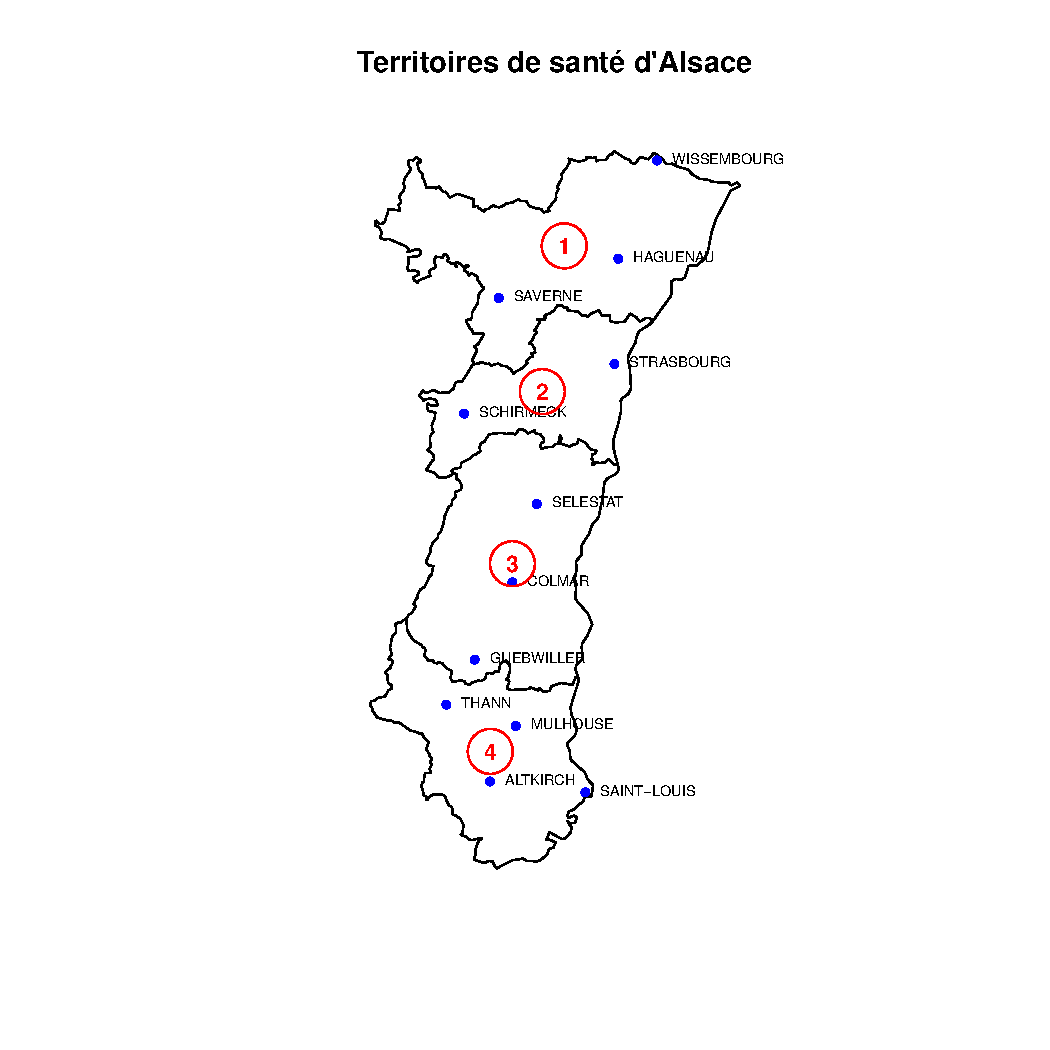
\includegraphics[width=\maxwidth]{figure/carte_secteurs_sanitaires-1} 

\end{knitrout}


\section{Les territoires de proximité}
%======================================

\index{Alsace!territoires de proximité}
\index{Territoires de proximité}

Il existe douze territoires de proximité:
\begin{enumerate}
  \item territoire 1: Wissembourg
  \item territoire 2: Haguenau
  \item territoire 3: Saverne
  \item territoire 4: Strasbourg
  \item territoire 5: Molsheim-Schirmeck
  \item territoire 6: Sélestat-Obernai
  \item territoire 7: Colmar
  \item territoire 8: Guebwiller
  \item territoire 9: Thann
  \item territoire 10: Mulhouse
  \item territoire 11: Altkirch
  \item territoire 12: Saint-Louis
\end{enumerate}

Chaque territoire dispose d'un établissement de santé de référence et un service d'urgence (sauf Schirmeck qui n'est pas labellisé).

% carte des territoires de santé
\begin{figure}[ht]
 \centering
 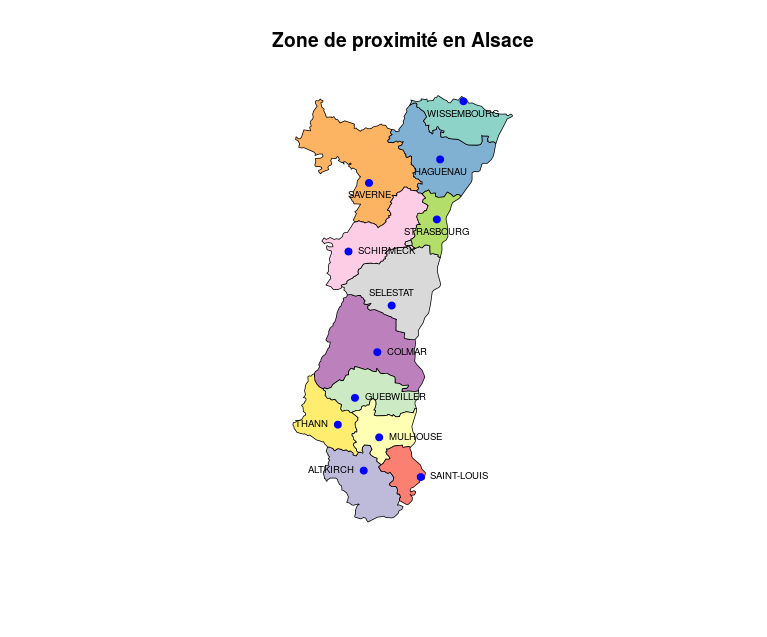
\includegraphics[height=15cm,keepaspectratio=true]{../doc/cartographie/RPU2013_Carto_Pop/figure/zp_avec_villes.png}
 % image.: 0x0 pixel, 0dpi, nanxnan cm, bb=
 \caption{L’Alsace compte 12 territoires de proximité}
 \label{fig:zp}
\end{figure}

\section{Démographie}
\subsection{Généralités}
\index{Alsace!démographie}

En France, les populations légales sont calculées par l'INSEE sur la base de définitions réglementaires à partir de recensement de la population. 
Les populations légales millésimées 2010 entrent en vigueur le 1\ier{} janvier 2013.  

\subsubsection{Le concept de population municipale}

Ce document utilise la \emph{Population municipale} \ref{Population_municipale} \index{Population@Population!municipale}  qui est la nouvelle dénomination de la population sans double compte et qui correspond à la notion de \emph{population} utilisée usuellement en statistique.
Le chiffre est donc inférieur de celui de la \emph{Population totale} qui est égale à la somme de la population municipale et de la population comptée à part d'une commune.
Les chiffres de l'INSEE sont résumés dans la table \footnote{http://www.insee.fr/fr/ppp/bases-de-donnees/recensement/populations-legales/france-regions.asp?annee=2010} \ref{pop2010} page \pageref{pop2010}.

\begin{table}
\begin{center}
\begin{tabular}{|c|c|}
\hline 
Région & Population\tabularnewline
\hline 
\hline 
France métropolitaine et DOM & 64 612 939\tabularnewline
\hline 
Dont France métropolitaine & 62 765 235\tabularnewline
\hline 
Alsace & 1 845 687\tabularnewline
\hline 
Bas-Rhin & 1 095 905\tabularnewline
\hline 
Haut-Rhin & 749 782\tabularnewline
\hline 
\end{tabular}
\caption[Populations légales 2010]{Populations légales 2010 des régions de France métropolitaine, Population
municipale (Source : Recensement de la population 2010 - Limites territoriales
au 1\ier{} janvier 2012) }
\label{pop2010}
\end{center}
\end{table}

\subsection{Classes d'âge}
Depuis la mise en place des serveurs régionaux, on a pris l'habitude de diviser la population en trois catégories selon l'age:
\begin{enumerate}
  \item Les moins de un an
  \item de 1 an à 75 ans
  \item les plus de 75 ans
\end{enumerate}

Les calculs sont effectués à partir du fichier \texttt{BTT\_TD\_POP1B\_2010} de l'INSEE qui recense l'ensemble de la population par commune et par tranches de un an. La version utilisée est celle du 1\ier{} janvier 2010 (tab.\ref{pop}). Le secteur de proximité de Strasbourg qui est aussi le plus peuplé, compte le plus grand nombre de personnes de 75 ans et plus (figure \ref{fig:75ans} page \pageref{fig:75ans})



\begin{table}
\begin{center}
\begin{tabular}{|l|l|r|r|}
  \hline
  Tranche d'age & Abréviation & Effectif & Pourcentage \\
  \hline
  \hline
   Moins de 1 an & pop0 & \np{21655} & 1.17 \\
   De 1 à 75 ans & pop1\_75 & \np{1677958} & 90.91 \\
   Plus de 75 ans& pop75 & \np{146074} & 7.91 \\
   \hline
   Total & pop\_tot & \np{1845687} & 100.00 \\
  \hline
\end{tabular}
\caption{Classe d'age en Alsace (janvier 2010)}
\label{pop}
\end{center}
\end{table}

% carte des plus de 75 ans
\begin{figure}[ht]
 \centering
 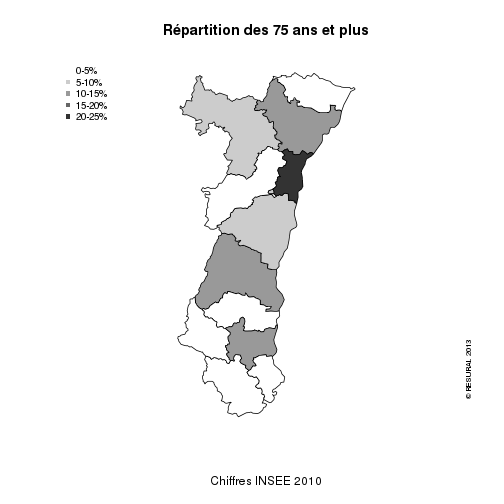
\includegraphics[height=15cm,keepaspectratio=true]{../doc/cartographie/RPU2013_Carto_Pop/figure/75ans.png}
 % image.: 0x0 pixel, 0dpi, nanxnan cm, bb=
 \caption[Répartition des 75 ans et plus]{Les personnes de 75 ans et plus en Alsace en fonction du territoire de proximité (en pourcentage du nombre total de 75 ans et plus).}
 \label{fig:75ans}
\end{figure}


\section{Les services d'accueil des urgences (SAU)}
%==================================================

\index{Services d'urgence!en Alsace}
\index{Alsace!services d'urgence}

L'autorisation de pratiquer la médecine d'urgence est délivrée par l'ARS en cohérence avec le schéma régional de l'organisation des soins (SROS) dont les dispositions pour la période 2012-2016 ont été précisées par l'arrêté du 30 janvier 2012 \cite{14} et du 23 mai 2013 \cite{15}.

Réglementairement, le CSP reconnaît deux types de structures pouvant être autorisées à prendre en charge directement des patients pouvant relever d'une situation d'urgence
\begin{enumerate}
  \item les structures d'urgence (SU). Le CSP reconnaît quatre types d'autorisations qui peuvent être dissociées:
    \begin{itemize}
      \item SAMU
      \item SMUR
      \item SU
      \item SU pédiatrique
    \end{itemize}

  \item les plateaux techniques spécialisés d'accès direct (PTSAD: article R 6123-32-6 CSP) qui sont de quatre types en Alsace:
    \begin{itemize}
      \item Urgences main
      \item Urgences cardiologiques
      \item Urgences neuro-vasculaires
      \item Polytraumatisés
    \end{itemize}
\end{enumerate}

On peut trouver des PTSAD avec une autorisation SU mais qui ne concerne que la spécialité du plateau technique, des PTSAD non labellisés SU, des SU non labellisés pédiatriques mais ayant une activité pédiatrique exclusive.

A la date du 23 mai 2013, l'Alsace compte 18 établissements ou structures autorisés pour l'activité de soins de médecine d'urgence (article R6123-1 du CSP) dont deux ayant une activité de PTDAD exclusive \cite{15}, et 1 établissement labellisé SU pédiatrique. Cette activité se répartit en:
\begin{itemize}
  \item 14 implantations "polyvalentes" (adultes et enfants): CH Wissembourg, CH Haguenau, CH Saverne, Clinique Sainte Odile, Clinique Sainte Anne, CH Sélestat, hôpital Pasteur, CH Guebwiller, CH Thann, CH Altkirch, Clinique des trois frontières, hôpital Emile Muller, clinique Diaconat-Fonderie.
  \item 2 implantations "adultes": Nouvel Hôpital Civil, hôpital de Hautepierre
  \item 3 implantations "pédiatriques": hôpital de Hautepierre, Clinique du Parc, Hôpital du Haserain.
  \item 2 implantations "urgences mains": clinique du Diaconat-Strasbourg, clinique Diaconat-Roosvelt.
\end{itemize}

Les HUS sont le seul établissement d'Alsace a posséder un SU pédiatrique labellisé. Les HUS ont également un service labellisé urgences main (FESUM) situé au CCOM d'Illkirch mais ce dernier n'a pas l'autorisation d'activité de soins de médecine d'urgence. Tous les services SOS Mains d'Alsace sont labellisé par la FESUM\footnote{Fédération Européenne des Services d'Urgence de la Main}.

% En pratique, à la question de savoir qui prend en charge 24h sur 24 des problèmes aigus de santé et/ou de permanence des soins, on se ramène a une liste de 14 établissements pratiquant la médecine d'urgence au sens où on l'entend communément. Trois établissements ont une activité multisite. Au final cela représente 18 sites. Les trois villes les plus importantes de la région concentrent la totalité des PTSAD.

L'activité de soins de médecine d'urgence se pratique au sein de ce qu'il est communément appelé services d'urgence (SU). Cette dénomination remplace la terminologie introduite par le SROS 2 qui distinguait alors les UPATOU, les POSU et les SAU. Cette nomenclature qui reposait sur une réalité avait été bien assimilée par les professionnels de santé et beaucoup continuent de l'utiliser, même si elle n'a plus cours officiellement. 

Le réseau prend également en compte la clinique Saint-Luc de Schirmeck (groupe hospitalier Saint Vincent) qui fait fonctionner une policlinique recevant plus de \np{8000} passages par an. Officiellement, cet établissement de santé ne dispose pas d' autorisation de type SU bien qu'elle en effectue la mission et est le seul établissement de proximité de la zone Molsheim-Schirmeck.

Sont officiellement labellisés 18 sites (en y incluant SOS main Diaconat mais pas la clinique St Luc). Ces données sont résumées dans le tableau \ref{tab:sualsace} page \pageref{tab:sualsace}


% \begin{landscape}
% \begin{table}
% \begin{center}
% \begin{tabular}{|c|c|c|c|c|c|c|c|c|c|}
% \hline 
% Territoire & ZProximité & Établissement & FINESS J & Site & FINESS G & SU & SU Ped & SMUR & SAMU\tabularnewline
% \hline 
% \hline 
%  \multirow{3}{*}{1} & Wissembourg & CH Wissembourg &  & id &  & oui &  & oui & \tabularnewline
% \cline{2-10} 
%  & Haguenau & CH Haguenau &  & id &  & oui &  & oui & \tabularnewline
% \cline{2-10} 
%  & Saverne & CH Saverne &  & id &  & oui &  & oui & \tabularnewline
% \hline 
% \multirow{7}{*}{2} & \multirow{6}{*}{Strasbourg} & \multirow{3}{*}{HUS} &  & NHC &  & oui &  &  & \tabularnewline
% \cline{4-10} 
%  &  &  &  & HTP &  & oui & oui & oui%
% \footnote{SMUR Péd.%
% } & \tabularnewline
% \cline{4-10} 
%  &  &  &  & PL &  &  &  & oui & oui\tabularnewline
% \cline{3-10} 
%  &  & Ste Anne &  & id &  & oui &  &  & \tabularnewline
% \cline{3-10} 
%  &  & Ste Odile &  & id &  & oui &  &  & \tabularnewline
% \cline{3-10} 
%  &  & Diaconat &  & id &  & oui%
% \footnote{SOS Mains%
% } &  &  & \tabularnewline
% \cline{2-10} 
%  & Schirmeck & St Luc &  & id &  &  &  &  & \tabularnewline
% \hline 
% \multirow{4}{*}{3} & Sélestat & CH Sélestat &  & id &  & oui &  & oui & \tabularnewline
% \cline{2-10} 
%  & \multirow{2}{*}{Colmar} & \multirow{2}{*}{CH Colmar} &  & HC &  & oui &  & oui & \tabularnewline
% \cline{4-10} 
%  &  &  &  & Parc &  &  & oui &  & \tabularnewline
% \cline{2-10} 
%  & Guebwiller & CH Guebwiller &  & id &  & oui &  &  & \tabularnewline
% \hline 
% \multirow{5}{*}{4} & \multirow{3}{*}{Mulhouse} & \multirow{2}{*}{CH Mulhouse} &  & EM &  & oui & oui & oui & oui\tabularnewline
% \cline{4-10} 
%  &  &  &  & St Louis &  & oui &  & oui%
% \footnote{antenne SMUR%
% } & \tabularnewline
% \cline{3-10} 
%  &  & Diaconat-F &  & id &  & oui &  &  & \tabularnewline
% \cline{2-10} 
%  & Thann & CH Thann &  & id &  & oui &  &  & \tabularnewline
% \cline{2-10} 
%  & Altkirch & CH Altkirch &  & id &  & oui &  &  & \tabularnewline
% \hline
% \end{tabular}
%  \caption[Structures d'urgence]{Services d'urgence d'Alsace}
% 
% \label{tab:sualsace}
% \end{center}
% \end{table}
% \end{landscape}


% Le tableau qui suit a été créé avec Lyx

\begin{landscape}
\begin{table}
\begin{center}

\selectlanguage{french}%
{\small{}}%
\begin{tabular}{|c|c|c|c|c|c|c|c|c|}
\hline 
{\small{Territoire}} & {\small{ZProximité}} & {\small{Etablissement}} & {\small{FINESS J}} & {\small{Site}} & {\small{FINESS G}} & {\small{SU}} & {\small{SAMU/SMUR}} & {\small{PTSAD}}\tabularnewline
\hline 
\hline 
\multirow{3}{*}{{\small{1}}} & {\small{Wissembourg}} & {\small{CH Wissembourg}} & {\small{670780543}} & {\small{Hôpital de la Lauter}} & {\small{670016237}} & {\small{polyvalent}} & {\small{SMUR}} & \selectlanguage{english}%
\selectlanguage{french}%
\tabularnewline
\cline{2-9} 
 & {\small{Haguenau}} & {\small{CH Haguenau}} & {\small{670780337}} & {\small{CH Haguenau}} & {\small{670000157}} & {\small{oui}} & {\small{SMUR}} & \selectlanguage{english}%
\selectlanguage{french}%
\tabularnewline
\cline{2-9} 
 & {\small{Saverne}} & {\small{CH Saverne}} & {\small{670780345}} & {\small{Hôpital Ste Catherine}} & {\small{670000165}} & {\small{oui}} & {\small{SMUR}} & \selectlanguage{english}%
\selectlanguage{french}%
\tabularnewline
\hline 
\multirow{10}{*}{{\small{2}}} & \multirow{9}{*}{{\small{Strasbourg}}} & \multirow{5}{*}{{\small{HUS}}} & \multirow{5}{*}{{\small{670780055}}} & {\small{NHC}} & {\small{670000025}} & {\small{oui}} & \selectlanguage{english}%
\selectlanguage{french}%
 & \selectlanguage{english}%
\selectlanguage{french}%
\tabularnewline
\cline{5-9} 
 &  &  &  & {\small{HTP Adulte}} & {\small{670783273}} & {\small{oui}} & {\small{SMUR Ped.}} & \selectlanguage{english}%
\selectlanguage{french}%
\tabularnewline
\cline{5-9} 
 &  &  &  & {\small{HTP Pédiatrie}} & {\small{670783273}} & {\small{oui}} & \selectlanguage{english}%
\selectlanguage{french}%
 & \selectlanguage{english}%
\selectlanguage{french}%
\tabularnewline
\cline{5-9} 
 &  &  &  & {\small{Pôle Logistique}} & \selectlanguage{english}%
\selectlanguage{french}%
 & \selectlanguage{english}%
\selectlanguage{french}%
 & \textbf{\small{SAMU}}{\small{/SMUR}} & \selectlanguage{english}%
\selectlanguage{french}%
\tabularnewline
\cline{5-9} 
 &  &  &  & {\small{CCOM}} & \selectlanguage{english}%
\selectlanguage{french}%
 & \selectlanguage{english}%
\selectlanguage{french}%
 & \selectlanguage{english}%
\selectlanguage{french}%
 & {\small{SOS mains}}\tabularnewline
\cline{3-9} 
 &  & {\small{Clinique de l'Orangerie}} & {\small{67000 0116}} & {\small{Clinique de l'Orangerie}} & {\small{670780170}} & \selectlanguage{english}%
\selectlanguage{french}%
 & \selectlanguage{english}%
\selectlanguage{french}%
 & {\small{USIC}}\tabularnewline
\cline{3-9} 
 &  & \multirow{2}{*}{{\small{Cliniques de Strasbourg}}} & {\small{670016211}} & {\small{Clinique Ste Odile}} & {\small{670016237}} & {\small{oui}} & \selectlanguage{english}%
\selectlanguage{french}%
 & \selectlanguage{english}%
\selectlanguage{french}%
\tabularnewline
\cline{4-9} 
 &  &  & {\small{670000108}} & {\small{Diaconat}} & {\small{670780162}} & {\small{SOS mains}} & \selectlanguage{english}%
\selectlanguage{french}%
 & \selectlanguage{english}%
\selectlanguage{french}%
\tabularnewline
\cline{3-9} 
 &  & \multirow{2}{*}{{\small{Groupe St Vincent}}} & \multirow{2}{*}{{\small{670014604}}} & {\small{Clinique Ste Anne}} & {\small{670780212}} & {\small{oui}} & \selectlanguage{english}%
\selectlanguage{french}%
 & \selectlanguage{english}%
\selectlanguage{french}%
\tabularnewline
\cline{2-2} \cline{5-9} 
 & {\small{Schirmeck}} &  &  & {\small{Clinique St Luc}} & {\small{670798636}} & \selectlanguage{english}%
\selectlanguage{french}%
 & \selectlanguage{english}%
\selectlanguage{french}%
 & \selectlanguage{english}%
\selectlanguage{french}%
\tabularnewline
\hline 
\multirow{5}{*}{{\small{3}}} & {\small{Sélestat}} & {\small{CH Sélestat}} & {\small{670780691}} & {\small{CH Sélestat}} & {\small{670000397}} & {\small{oui}} & {\small{SMUR}} & \selectlanguage{english}%
\selectlanguage{french}%
\tabularnewline
\cline{2-9} 
 & \multirow{3}{*}{{\small{Colmar}}} & \multirow{2}{*}{{\small{CH Colmar}}} & \multirow{2}{*}{{\small{680000973}}} & {\small{Louis Pasteur}} & {\small{680000684}} & {\small{oui}} & {\small{SMUR}} & \selectlanguage{english}%
\selectlanguage{french}%
\tabularnewline
\cline{5-9} 
 &  &  &  & {\small{Clinique du Parc}} & {\small{680001245}} & \selectlanguage{english}%
\selectlanguage{french}%
 & \selectlanguage{english}%
\selectlanguage{french}%
 & \selectlanguage{english}%
\selectlanguage{french}%
\tabularnewline
\cline{3-9} 
 &  & {\small{GHCA}} & {\small{680016011}} & {\small{Hôpital Schweitzer}} & {\small{680001195}} & \selectlanguage{english}%
\selectlanguage{french}%
 & \selectlanguage{english}%
\selectlanguage{french}%
 & {\small{USIC}}\tabularnewline
\cline{2-9} 
 & {\small{Guebwiller}} & {\small{CH Guebwiller}} & {\small{680000005}} & {\small{Hôpital Charles Haby}} & {\small{680000700}} & {\small{oui}} & \selectlanguage{english}%
\selectlanguage{french}%
 & \selectlanguage{english}%
\selectlanguage{french}%
\tabularnewline
\hline 
\multirow{7}{*}{{\small{4}}} & \multirow{4}{*}{{\small{Mulhouse}}} & \multirow{2}{*}{{\small{CH Mulhouse}}} & \multirow{2}{*}{{\small{680000486}}} & {\small{Emile Muller}} & {\small{680000627}} & {\small{oui}} & \textbf{\small{SAMU}}{\small{/SMUR}} & \selectlanguage{english}%
\selectlanguage{french}%
\tabularnewline
\cline{5-9} 
 &  &  &  & {\small{Hasenrain}} & {\small{680000627}} & \selectlanguage{english}%
\selectlanguage{french}%
 & \selectlanguage{english}%
\selectlanguage{french}%
 & \selectlanguage{english}%
\selectlanguage{french}%
\tabularnewline
\cline{3-9} 
 &  & \multirow{2}{*}{{\small{Fondation du Diaconat}}} & {\small{680000643}} & {\small{Diaconat Fonderie}} & {\small{680000320}} & {\small{oui}} & \selectlanguage{english}%
\selectlanguage{french}%
 & \selectlanguage{english}%
\selectlanguage{french}%
\tabularnewline
\cline{4-9} 
 &  &  & \selectlanguage{english}%
\selectlanguage{french}%
 & {\small{Diaconat Roosvelt}} & {\small{680000494}} & {\small{SOS mains}} & \selectlanguage{english}%
\selectlanguage{french}%
 & \selectlanguage{english}%
\selectlanguage{french}%
\tabularnewline
\cline{2-9} 
 & {\small{Thann}} & {\small{CH Thann}} & {\small{680000437}} & {\small{Hôpital St Jacques}} & {\small{680000601}} & {\small{oui}} & \selectlanguage{english}%
\selectlanguage{french}%
 & \selectlanguage{english}%
\selectlanguage{french}%
\tabularnewline
\cline{2-9} 
 & {\small{Altkirch}} & {\small{CH Altkirch}} & {\small{680000395}} & {\small{CH St Morand}} & {\small{680000395}} & {\small{oui}} & \selectlanguage{english}%
\selectlanguage{french}%
 & \selectlanguage{english}%
\selectlanguage{french}%
\tabularnewline
\cline{2-9} 
 & {\small{Saint-Louis}} & {\small{Clinique des 3 frontières}} & {\small{680000049}} & {\small{C3F}} & {\small{680020096}} & {\small{oui}} & \selectlanguage{english}%
\selectlanguage{french}%
 & \selectlanguage{english}%
\selectlanguage{french}%
\tabularnewline
\hline 
\end{tabular}\selectlanguage{english}%

\caption[Structures d'urgence]{Services d'urgence d'Alsace}
\label{tab:sualsace}
\end{center}
\end{table}
\end{landscape}



\begin{figure}[ht]
 \centering
\begin{knitrout}
\definecolor{shadecolor}{rgb}{0.969, 0.969, 0.969}\color{fgcolor}
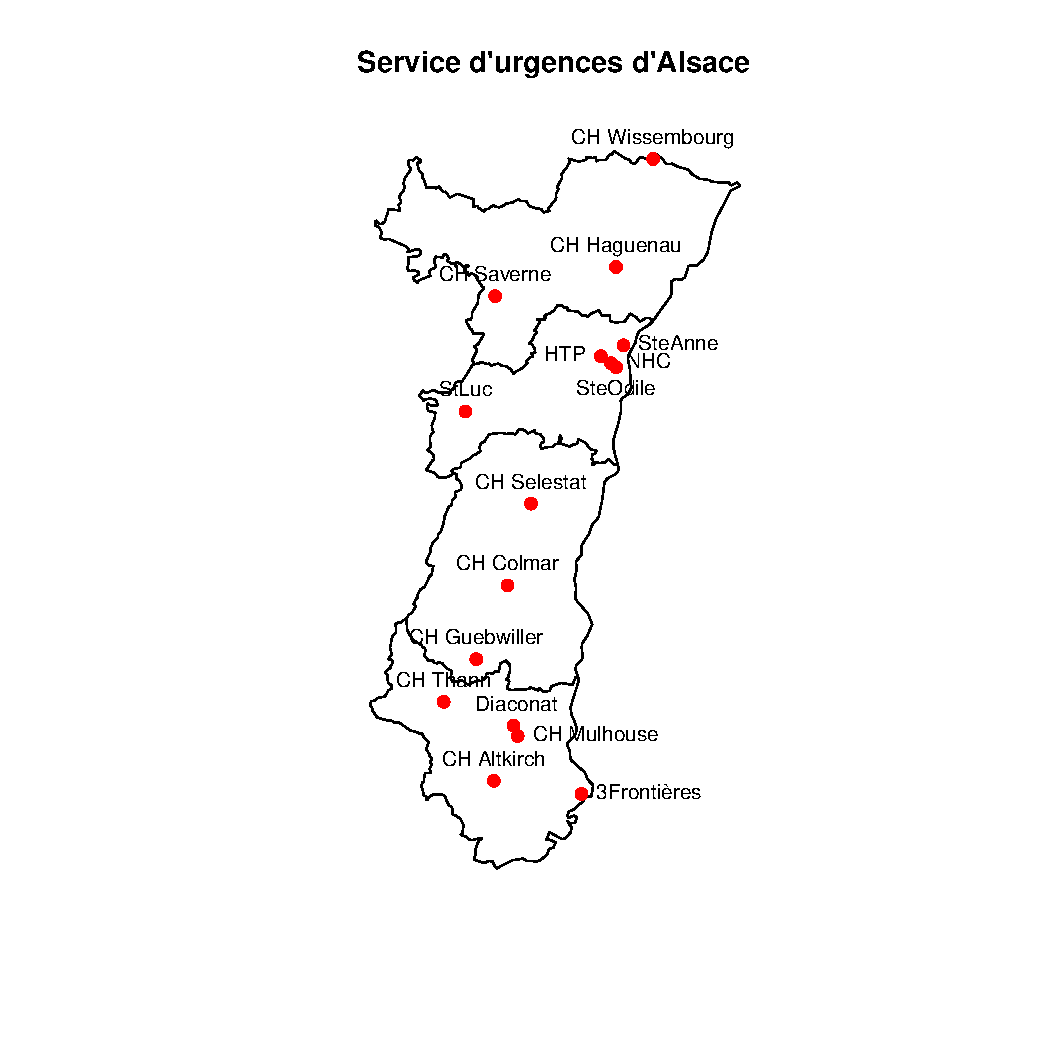
\includegraphics[width=\maxwidth]{figure/carte_sau_2-1} 

\end{knitrout}
 \caption[Services d'urgence d'Alsace]{Implantation des services d'urgence en Alsace.}
 \label{fig:su_alsace}
\end{figure}



% \begin{table}
% \begin{center}
% \begin{tabular}{|c|c|c|c|l|}
%   \hline
% & FINESS utilisé & FINESS géographique & FINESS Juridique & Structure \\
%   \hline
%   \hline
% 1 & 670780055 &   & 670780055 & HUS \\
% 2 & 670780543 & 670000272 & 670780543 & CH Wissembourg \\
% 3 & 670000397 & 670000397  & 670780691 & CH Sélestat \\
% 4 & 670780337 & 670000157 & 670780337 & CH Haguenau \\
% 5 &   & 670000165 & 670780345 & CH Saverne \\
% 6 & 670016237  & 670016237  & 670016211 & Clinique Ste Odile \\
% 7 &   & 670780212 & 670014604 & Clinique Ste Anne \\
% 8 & 680000973 & 680000684 & 680000973 & CH Colmar \\
% 9 & 680000197  & 680000197  & 680000049 & Clinique des trois frontières \\
% 10 & 680000486 & 680000544  & 680000395 & CH Altkirch \\
% 11 & 680000700 & 680000700 & 680001005 & CH Guebwiller \\
% 12 & 680000627 & 680000627 & 680000486 & CH Mulhouse FG \\
% 13 &   & 680000601 & 680000437 & CH Thann \\
% 14 &   & 680000320  & 680000643 & Diaconat-Fonderie (St Sauveur) \\
% \hline
% \end{tabular}
% \caption{Service d'accueil des urgences d'Alsace}
% \label{summary}
% \end{center}
% \end{table}

\section{Les plateaux techniques spécialisés à accès direct (PTSAD)} 

Les PTSAD relevant de l'article R 6123-32-6 CSP doivent adhérer à un réseau d'urgence mais ne sont pas tenus de produire des RPU. Sont concernés en Alsace:
\begin{itemize}
\item Urgences main: Diaconat-Strasbourg, Diaconat-Roosvelt, CCOM.
\item Urgences cardiologiques: clinique de l'Orangerie, clinique Schweitzer (GHCA).
\item Urgences neuro-vasculaires: HTP, CH Colmar, CH Mulhouse, (CH Haguenau).
\item Polytraumatisés: HTP, CH Colmar, CH Mulhouse.
\end{itemize}

\newpage
\chapter{RESURAL}

% resural.Rnw
\index{RESURAL}

Le réseau des urgences en Alsace (RESURAL) est une association à but non lucratif, de droit local Alsace-Moselle, dont les statuts sont déposés au tribunal d'instance de Strasbourg. Le réseau a été fondé en août 2008. En sont membres de droit les services d'urgence intra et extra-hospitaliers, adultes et pédiatriques, possédant une autorisation d'exercer cette spécialité, délivrée par l'agence régionale de santé (ARS). \index{ARS}

Elle est domiciliée aux Hôpitaux Universitaires de Strasbourg.

Elle est dirigée par un conseil d'administration et représentée par son président, le Docteur Bruno Goulesque.

Son fonctionnement est assuré par une équipe de coordination, composée d'un médecin coordinateur à mi-temps et d'une assistante à mi-temps. Cette équipe est opérationnelle depuis le 1\ier{} février 2013.

\newpage
\chapter{L'observatoire des urgences en Alsace (ORUDAL)}

% orudal.Rnw

L'observatoire des urgences en Alsace (ORUDAL) est une structure informelle animée par le réseau des urgences en Alsace.
\index{ORUDAL}
\index{Observatoire des urgences en Alsace}

Il est composé des organismes suivants:
\begin{enumerate}
  \item RESURAL \index{RESURAL}
  \item ARS Alsace
  \item CIRE-InVS
  \item Alsace e-santé
  \item CMUNE
\end{enumerate}


\section*{Les partenaires}

  \subsection*{Agence Régionale de Santé}
    \index{ARS}
    
  \subsection*{Alsace e-santé}
    \index{Alsace e-santé}
    
  \subsection*{CIRE-INVS}
    \index{CIRE-INVS}
    
  \subsection*{Collège de médecine d'urgence (CMUNE)}
    \index{CMUNE}

\section*{FEDORU}
  \index{FEDORU}
  
La fédération des observatoires des urgences et structures apparentées a été créée en octobre 2013 à l'initiative de quelques organismes régionaux dont RESURAL sur une proposition de l'ORUPACA \index{ORUPACA}

\newpage
\chapter{Le Résumé du passage aux urgences}

% rpu.Rnw

\index{RPU}
\index{Résumé du passage aux urgences}

La création du résumé des passages aux urgences (RPU) remonte à 2002 \cite{11}. Sur la base d'un projet pilote mené par l'ORUMIP, la DHOS, à l'initiative de son directeur Edouard Couty, lance sur la base du volontariat, la collecte des RPU.

\section*{RPU}

% Les Résumés de Passage aux Urgences (RPU) ont été transmis par le Centre Hospitalier de Sélestat à partir de 2008. 
% La table \emph{rpu} du serveur de test comporte nrow(d2) lignes et ncol(d2) colonnes. La période érudiée couvre toute l'année 2009 s'étend (du d2$date_entree[1] au d2$date_entree[nrow(d2)]), ce qui correspond à toutes les entrées de cette année. Les RPU sont saisis selon la version 5 du cahier des charges transmis par l'INVS (version du 31 janvier 2007).
% \\
Chaque passage aux urgences donne lieu à la création d'un RPU qui collecte les informations suivantes:
\begin{enumerate}
  \item l'établissement de santé, siège du SAU (FINESS géographique)
  \item code postal de résidence
  \item commune de résidence
  \item date de naissance
  \item sexe
  \item date et heure d'entrée
  \item mode d'entrée
  \item provenance du patient
  \item mode de transport
  \item mode de prise en charge
  \item le motif de recours aux urgences
  \item la gravité
  \item le diagnostic principal
  \item le(s) diagnostic(s) associé(s)
  \item les actes médicaux
  \item le mode de sortie
  \item l'orientation du patient
  \item date et heure de sortie
\end{enumerate}

%%%%%%%%%%%%%%
\subsubsection{L'identifiant (ID)}
%%%%%%%%%%%%%%

Il s'agit d'un code unique caractérisant le RPU. Il ne fait pas partie de la définition de l'INVS. 
Il a été rajouté par SAGEC à l'origine du serveur régional pour retrouver l'enregistrement en cas de problème et faciliter la liaison avec d'autres rubriques comme les diagnostics associés.

%%%%%%%%%%%%%%
\subsubsection{L'établissement de santé}
%%%%%%%%%%%%%%

\index{FINESS}
Il est identifié par son numéro FINESS. Le schéma de l'INVS ne précise pas quel FINESS utiliser et on trouve des FINESS juridiques et géographiques. Nous recommandons d'utiliser le FINESS géographique qui permet d'identifier la structure d'origine quand il s'agit d'établissements multisites.

%%%%%%%%%%%%%%
\subsubsection{Le code postal de résidence}
%%%%%%%%%%%%%%

\index{Code postal}
Lorsque le lieu de résidence se situe hors des limites du territoire national, il faut indiquer par convention $99999$.
Si le code postal précis est inconnu : le numéro du département suivi de 999.
Pour les malades résidant hors de France : 99 suivi du code INSEE du pays \footnote{http://www.insee.fr/fr/methodes/nomenclatures/cog/pays.asp}.
Si le département ou le pays de résidence est inconnu : 99999.
Deux communes peuvent avoir le même code postal (Vendenheim et Eckwersheim) et une commune importante peut avoir plusieurs codes postaux(Strasbourg).

%%%%%%%%%%%%%%
\subsubsection{La commune de résidence}
%%%%%%%%%%%%%%

\index{Commune de résidence}
En l'absence de code INSEE, il convient de respecter les recommandations suivantes:
\begin{itemize}
  \item utiliser exclusivement des lettres majuscules
  \item ne pas utiliser de caractères accentués
  \item remplacer les blancs par un trait d'union (VIR-AU-VAL)
\end{itemize}

%%%%%%%%%%%%%%
\subsubsection{la date de naissance}
%%%%%%%%%%%%%%

\index{Date de naissance}
\index{Age}
Elle comporte l'année, le mois et le jour de naissance, ce qui permet de calculer l'âge au moment de l'admission. Dans ce document on utilise l'âge par génération ou âge atteint dans l'année (et non pas l'âge révolu). Comme toutes les dates il est préférable d'utiliser la norme ISO 8601 (AAAA-MM-JJ HH:MM:SS).

%%%%%%%%%%%%%%
\subsubsection{le mode d'entrée}
%%%%%%%%%%%%%%

\index{Mode d'entrée}
Trois codes imposés:
\begin{itemize}
  \item \textbf{6} Mutation
  \item \textbf{7} Transfert
  \item \textbf{8} Domicile
\end{itemize}


%%%%%%%%%%%%%%
\subsubsection{la provenance}
%%%%%%%%%%%%%%

\index{Provenance}
Le RPU propose deux séries de code selon que le patient provient d'un établissement de santé ou du domicile. Si l'origine est un établissement:
\begin{itemize}
  \item \textbf{1} En provenance d'une unité de soins de courte durée (MCO) 
  \item \textbf{2} En provenance d'une unité de soins de suite ou de réadaptation
  \item \textbf{3} En provenance d'une unité de soins de longue durée
  \item \textbf{4} En provenance d'une unité de psychiatrie
\end{itemize}
Si le patient vient du domicile:
\begin{itemize}
  \item \textbf{7} Prise en charge aux urgences autres que pour des raisons organisationnelles
  \item \textbf{8} Prise en charge aux urgences pour des raisons organisationnelles \footnote{Ce code ne fait pas partie des codes du PMSI. Il a été créé spécifiquement pour le RPU.}
    \begin{itemize}
      \item patient re-convoqué par le même service d’urgence pour des soins à distance de la prise en charge initiale (surveillance de plâtre, réfection de pansements, rappel de vaccination)
      \item patient déjà attendu avant sa prise en charge aux urgences dans un autre service et transitant aux urgences pour faciliter l’enregistrement administratif ou la réalisation des premiers examens complémentaires à la prise en charge qui va suivre.
    \end{itemize}
\end{itemize}

Les codes \textbf{Provenance} 1 à 4 sont incompatibles avec \textbf{Mode d'entrée} 8. De même les codes \textbf{Provenance} 7 et 8 sont incompatibles avec \textbf{Mode d'entrée} 6 et 7.


%%%%%%%%%%%%%%
\subsubsection{Le mode de transport}
%%%%%%%%%%%%%%

\index{Mode de transport}
Ce sont des codes textuels précisant le moyen utilisé pour se rendre aux urgences.

%%%%%%%%%%%%%%
\subsubsection{la prise en charge durant le transport}
%%%%%%%%%%%%%%

\index{Prise en charge durant le transport}
Ce sont des codes textuels précisant s'il y avait un accompagnement médical ou paramédical durant le transport.

%%%%%%%%%%%%%%
\subsubsection{le motif de recours aux urgences}
%%%%%%%%%%%%%%

\index{motif de recours}
Il faut utiliser l'un des motifs de recours préconisé par le ministère de la santé \cite{13} et codifiés par la SFMU. La dernière version est la version de juin 2013 du thésaurus de la SFMU accessible sur le site internet de cette dernière. Il comporte une liste d'environ $150$ recours avec leur équivalence CIM10.


%%%%%%%%%%%%%%
\subsubsection{Le mode de sortie}
%%%%%%%%%%%%%%

\index{mode de sortie}
\index{retour à domicile}
\label{ref:sortie}
Les patients quittent les urgences soit parce qu'ils ne nécessitent pas d'hospitalisation (c'est un \emph{retour à domicile}), soit parce qu'ils sont hospitalisés dans la structure hospitalière (c'est une \emph{mutation}\index{mutation}) ou dans un autre établissement (on parle alors de \emph{transfert}\index{transfert}). Enfin il peut s'agir d'un \emph{décès}\index{décès} dans le service d'urgence.

\begin{itemize}
  \item « 6 » Mutation : le malade est hospitalisé vers une autre unité médicale de la même
entité juridique \footnote{Dans les établissements privés visés aux alinéas d et e de l'article L162-22-6 du code de la sécurité sociale (CSS), si le patient provient d’un autre établissement de la même entité juridique, le mode de sortie à utiliser est le 7}
  \item « 7 » Transfert : le malade est hospitalisé dans une autre entité juridique
  \item « 8 » Domicile : le malade retourne au domicile ou son substitut, tel une
structure d'hébergement médico-social.
  \item « 9 » Décès : le malade décède aux urgences
\end{itemize}

Cette rubrique est détaillée par les items \emph{destination} et \emph{orientation}

%%%%%%%%%%%%%%
\subsubsection{Destination}
%%%%%%%%%%%%%%

En cas de sortie par mutation ou transfert, il peut s'agir:
\begin{itemize}
  \item « 1 » Hospitalisation dans une unité de soins de courte durée (MCO)\index{MCO}
  \item « 2 » Hospitalisation dans une unité de soins de suite ou de réadaptation (SSR)\index{SSR}
  \item « 3 » Hospitalisation dans une unité de soins de longue durée (SLD)\index{SLD}
  \item « 4 » Hospitalisation dans une unité de psychiatrie (PSY)\index{PSY}
\end{itemize}
Les codes 1 à 4 sont incompatibles avec \textbf{mode de sortie} = \textbf{domicile}

En cas de sortie au domicile
\begin{itemize}
  \item « 6 » Retour au domicile dans le cadre d’une hospitalisation à domicile (HAD)\index{HAD}
  \item « 7 » Retour vers une structure d'hébergement médico-social (HMS)\index{HMS}
\end{itemize}
Les codes 6 et 7 sont incompatibles avec \textbf{mode de sortie} = \textbf{mutation, transfert} ou \textbf{décès}.

On notera que dans cette formulation, le retour à domicile "normal" est implicite et celà génère une ambiguité car si la rubrique est laissée libre, on ne sait pas s'il s'agit d'une non-réponse ou d'un retour simple à domicile.

%%%%%%%%%%%%%%
\subsubsection{Orientation}
%%%%%%%%%%%%%%

\index{orientation}
L'orientation précise le devenir ou les circonstances associées. Cette rubrique est complémentaire du \emph{mode de sortie}. Malheureusement, elle souffre de la même limitation:le retour à domicile simple est implicite.

\begin{enumerate}
  \item En cas de sortie par mutation ou transfert
    \begin{itemize}
      \item « HDT » hospitalisation sur la demande d’un tiers
      \item « HO » hospitalisation d’office
      \item « SC » hospitalisation dans une unité de Surveillance Continue
      \item « SI » hospitalisation dans une unité de Soins Intensifs
      \item « REA » hospitalisation dans une unité de Réanimation
      \item « UHCD » hospitalisation dans une unité d’hospitalisation de courte durée
      \item « MED » hospitalisation dans une unité de Médecine hors SC, SI, REA
      \item « CHIR» hospitalisation dans une unité de Chirurgie hors SC, SI, REA
      \item « OBST» hospitalisation dans une unité d’Obstétrique hors SC, SI, REA
    \end{itemize}

  \item En cas de sortie au domicile
    \begin{itemize}
      \item « FUGUE » sortie du service à l’insu du personnel soignant
      \item « SCAM » sortie contre avis médical
      \item « PSA » partie sans attendre prise en charge
      \item « REO » réorientation directe sans soins (ex vers consultation spécialisée ou   lorsque le service d’accueil administratif est fermée)
    \end{itemize}

\end{enumerate}

Selon le cas ces codes sont incompatibles avec un \textbf{mode de sortie} à domicile ou une hospitalisation.


% ************************
% *                      *  
% *      PARTIE 2        * 
% *                      *
% ************************
\part{Activité des services d'urgence d'Alsace}


\newpage
\chapter{Qualité des RPU en 2013} % ex chapitre "les acteurs"

% acteurs.Rnw

% penser au secteur libéral

\section{Exhaustivité quantitative}


On définit l'\emph{exhaustivité quantitative} \index{exhaustivité quantitative (def.)} comme le nombre de RPU transmis par rapport au nombre de passages réels.
Les données proviennent des RPU produits par les hôpitaux d'Alsace ayant l'autorisation de faire fonctionner un service d'urgence (SU). La liste des structures hospitalières ayant fournit des informations alimentant le présent rapport est fournie par la table \ref{tab1}, page \pageref{tab1}.

Tous ces hôpitaux fournissent des données depuis le premier janvier 2013 sauf le CH Saverne qui a commencé en Juillet 2013.

Quatre structures ne fournissent pas encore de RPU. Il s'agit de la clinique Sainte-Anne à Strasbourg (Groupe hospitalier Saint-Vincent), du Centre Hospitalier de Thann, de la clinique du Diaconat à Strasbourg et de la clinique Roosvelt à Mulhouse.

Certaines données peuvent être recoupées avec celles du serveur régional mis en place en 2006 par l'ARS: 

% \fbox{Voir SAU2013}

% latex table generated in R 3.1.2 by xtable 1.7-1 package
% Sat Nov  8 20:44:51 2014
\begin{table}[ht]
\centering
\begin{tabular}{|l|r|r|l|r|}
  \hline
 & n & \% & Hôpitaux & Date d'inclusion \\ 
  \hline
3Fr & 15688 & 4.56 & Clinique des 3 frontières & 01/01/2013 \\ 
  Alk & 10861 & 3.16 & CH Altkirch & 01/01/2013 \\ 
  Col & 64758 & 18.82 & CH Colmar & 01/01/2013 \\ 
  Dia & 29469 & 8.56 & Diaconat Fonderie & 01/01/2013 \\ 
  Geb & 15103 & 4.39 & CH Guebwiller & 01/01/2013 \\ 
  Hag & 34414 & 10 & CH Haguenau & 01/01/2013 \\ 
  Hus & 37018 & 10.76 & Hôpitaux Universitaires de Strasbourg & 01/01/2013 \\ 
  Mul & 56195 & 16.33 & CH Mulhouse & 07/01/2013 \\ 
  Odi & 25963 & 7.55 & Clinique Ste Odile & 01/01/2013 \\ 
  Sel & 29534 & 8.58 & CH Sélestat & 01/01/2013 \\ 
  Wis & 12646 & 3.68 & CH Wissembourg & 01/01/2013 \\ 
  Sav & 12424 & 3.61 & CH Saverne & 23/07/2013 \\ 
   \hline
\end{tabular}
\caption[Structures hospitalières participantes en 2013]{Structures hospitalières participantes en 2013. Tous les paticipants fournissent des données depuis le 1/1/2013 sauf le CH Saverne.} 
\label{tab1}
\end{table}


\section{Exhaustivité qualitative} \index{exhaustivité qualitative (def.)} 

L'\emph{exhaustivité qualitative} correspond à la fois à la complétude des items et à la cohérence de réponses.

Les informations de nature administrative (code postal, commune d'origine, sexe, date de naissance,\dots ) sont correctement renseignées avec une exhaustivité de $100\%$.

Les données à caractère plus médical comme le motif de consultation ou le diagnostic principal ont une exhaustivité moins bonne, de l'ordre de $70\%$. Les motifs DESTINATION et ORIENTATION sont à pondérer en fonction du MOTIF\_SORTIE. En effet la structure du RPU fait que par défaut, tous les retours à domicile génèrent automatiquement un non réponse pour les motifs DESTINATION et ORIENTATION qui ne concernent que les patients hospitalisés.

% latex table generated in R 3.1.2 by xtable 1.7-1 package
% Sat Nov  8 20:44:52 2014
\begin{table}[ht]
\centering
\begin{tabular}{|l|r|}
  \hline
 & \% \\ 
  \hline
id & 0.00 \\ 
  CODE\_POSTAL & 0.00 \\ 
  COMMUNE & 0.00 \\ 
  ENTREE & 0.00 \\ 
  EXTRACT & 0.00 \\ 
  FINESS & 0.00 \\ 
  NAISSANCE & 0.00 \\ 
  SEXE & 0.00 \\ 
  AGE & 0.00 \\ 
  secteur & 0.00 \\ 
  SORTIE & 8.82 \\ 
  MODE\_ENTREE & 9.57 \\ 
  MODE\_SORTIE & 13.88 \\ 
  GRAVITE & 14.24 \\ 
  TRANSPORT & 23.06 \\ 
  TRANSPORT\_PEC & 26.26 \\ 
  DP & 33.58 \\ 
  PROVENANCE & 35.75 \\ 
  MOTIF & 36.29 \\ 
  DESTINATION & 78.79 \\ 
  ORIENTATION & 80.14 \\ 
   \hline
\end{tabular}
\caption{Données manquantes en 2013 en pourcentage du total des réponses. Les données administrative du RPU, notemment les paramètres saisis dès l'arrivée du patient sont exhaustifs. Par contre les données de suivis et médicales sont moins complètes. Les motifs DESTINATION et ORIENTATION sont à pondérer en fonction du MOTIF SORTIE (voir texte).} 
\label{tab2}
\end{table}


Les informations sont résumées dans la table \ref{tab2}, page \pageref{tab2}.

\section{Diagramme de complétude}

On peut représenter sous forme d'un diagramme en radar (ou toile d'araignée) l'exhaustivité qualitative des données. Chaque item du RPU est représenté par le rayon d'une roue, gradué de 0 à 100\%. Sur chaque rayon, les points obtenus sont reliés entre eux pour dessiner un polygone qui figue la physionomie de l'ensemble des données.

\begin{knitrout}
\definecolor{shadecolor}{rgb}{0.969, 0.969, 0.969}\color{fgcolor}\begin{kframe}
\begin{verbatim}
           id   CODE_POSTAL       COMMUNE   DESTINATION            DP 
          0.0           0.0           0.0          78.8          33.6 
       ENTREE       EXTRACT        FINESS       GRAVITE   MODE_ENTREE 
          0.0           0.0           0.0          14.2           9.6 
  MODE_SORTIE         MOTIF     NAISSANCE   ORIENTATION    PROVENANCE 
         13.9          36.3           0.0          80.1          35.8 
         SEXE        SORTIE     TRANSPORT TRANSPORT_PEC           AGE 
          0.0           8.8          23.1          26.3           0.0 
\end{verbatim}
\end{kframe}
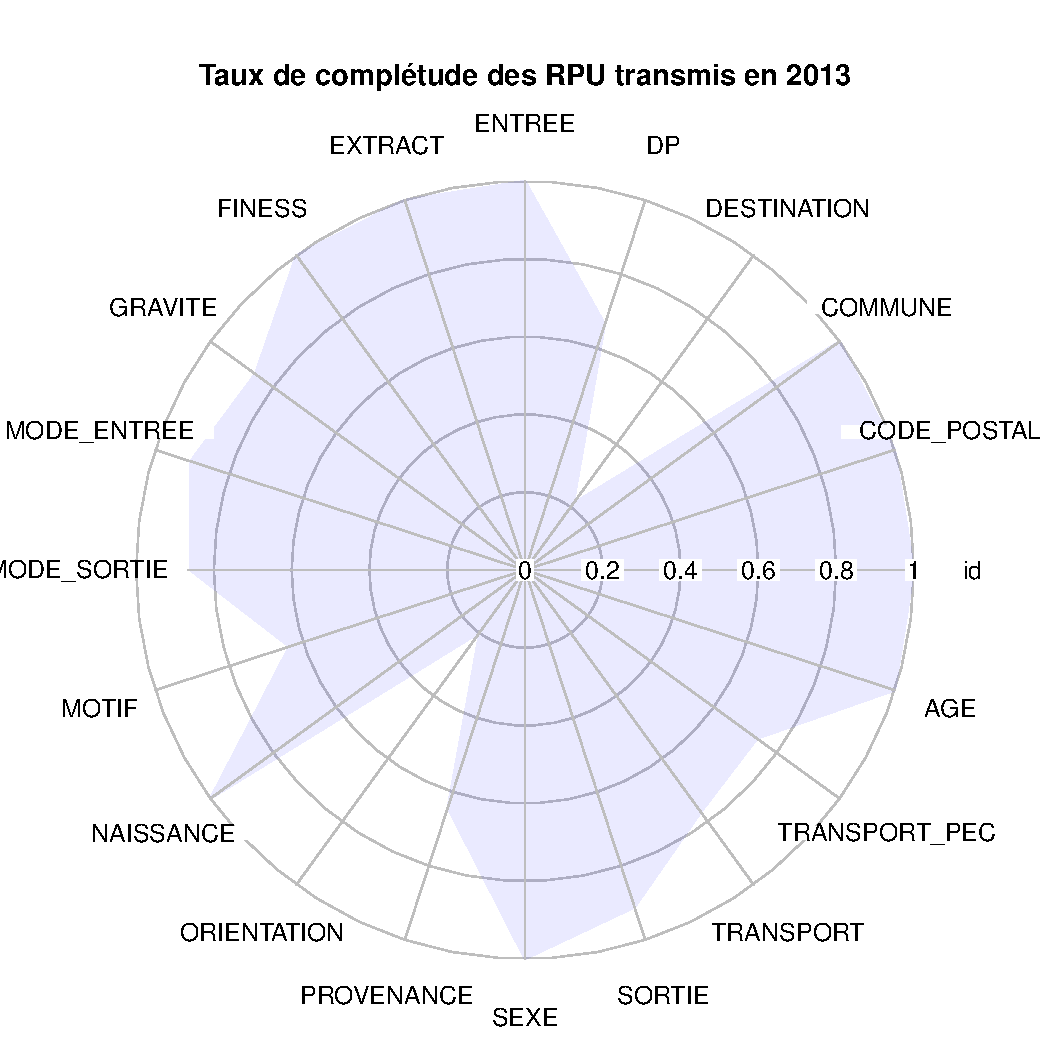
\includegraphics[width=\maxwidth]{figure/radar-1} 

\end{knitrout}

Le renseignement des items varie entre $20\%$ et $100\%$. Cependant ces données sont à interpréter avec prudence. Ainsi l'item 4 qui correspond au mode de sortie ne distingue pas les non réponses des vrais retours à domicile (se reporter à la discussion page \pageref{ref:sortie})

Les diagrammes de complétude propres à chaque établissement figurent au chapitre correspondant au service d'urgence.

Pour les items \textbf{Orientation} et \textbf{Destination}, il s'agit d'un taux de réponse brut. Ce dernier doit être corrigé en soustrayant les patients rentrés à domicile pour lesquels ces deux items n'ont pas de sens. Le chiffre corrigé apparaît dans les diagrammes de complétude spécifiques d'un service d'urgence (Partie quatre: Activité par service d'urgence page \pageref{partie4})

\newpage
\chapter{Activité régionale totale}

NOTE: dans les lignes qui suivent le terme \textbf{Passage} fait référence aux primo-passages ayant donnés lieu à la création d'un RPU (et non pas à la totalité des passages que peut enregistrer un service d'urgence.) \index{Passages (def.)}

\section{Nombre total de passages}

% activite_regionale.Rnw ou Activité régionale totale

% NOTE: il n'est pas nécessaire de rendre toutes les figures flottantes. Voir notamment les références:
% - http://www.tex.ac.uk/cgi-bin/texfaq2html?label=figurehere
% - http://www.tex.ac.uk/cgi-bin/texfaq2html?label=floats
% - http://www.tex.ac.uk/cgi-bin/texfaq2html?label=tmupfl

%on fabrique un objet **a** qui fait la somme par date des passages aux urgences:


% vérification:
%   a[1:10]
% 2013-01-01 2013-01-02 2013-01-03 2013-01-04 2013-01-05 2013-01-06 2013-01-07 2013-01-08 2013-01-09 2013-01-10 
%        884        801        686        704        722        691        876        694        683        673 
% On supprime l'enregistrement 211 correspondant au 31 juillet et qui ne contient que 2 éléments:
%a[211]  2013-07-31 2 

% Min. 1 st Qu.  Median    Mean 3rd Qu.    Max. 
%   642.0   848.0   895.5   883.2   957.0  1050.0 

En \ancourante les SU produisant des RPU ont déclaré \np{344 073} passages au 31 décembre 2013, 
soit une moyenne de \np{945} RPU par jour (extrêmes 675 et \np{1 180})

RPU par territoire de santé:
\index{Territoires de santé!nombre de RPU}



\begin{table}[ht]
\centering
\begin{tabular}{crr}
  \hline
 Territoire & RPU déclarés & Données SAE\\ 
  \hline
  1 & \np{59 484} & \np{83 722} \\ 
  2 & \np{62 981} & \np{144 095} \\ 
  3 & \np{109 395} & \np{115 459} \\ 
  4 & \np{112 213} & \np{150 045} \\ 
   \hline
\end{tabular}
\end{table}

Les valeurs du fichier SAE permettent d'avoir une idée de l'exhaustivité quantitative des RPU transmis.
Les données RPU du secteur 2 sont très sous-estimées car il manque celles de la Clinique Sainte-Anne, des urgences pédiatriques de Hautepierre ainsi qu'une part importante des RPU des urgences adulte des HUS. Pour le secteur 1, il manque 6 mois de données du CH Saverne. Les données du CH Thann manquent pour le secteur 4. Seul le secteur 3 a un nombre de RPU cohérent avec les données SAE. Au total le fichier SAE répertorie \np{493 321} passages aux urgences soit \np{149 248} RPU manquants (30 \%).

%affichage du graphique
%\begin{figure}
\begin{center}
\begin{knitrout}
\definecolor{shadecolor}{rgb}{0.969, 0.969, 0.969}\color{fgcolor}
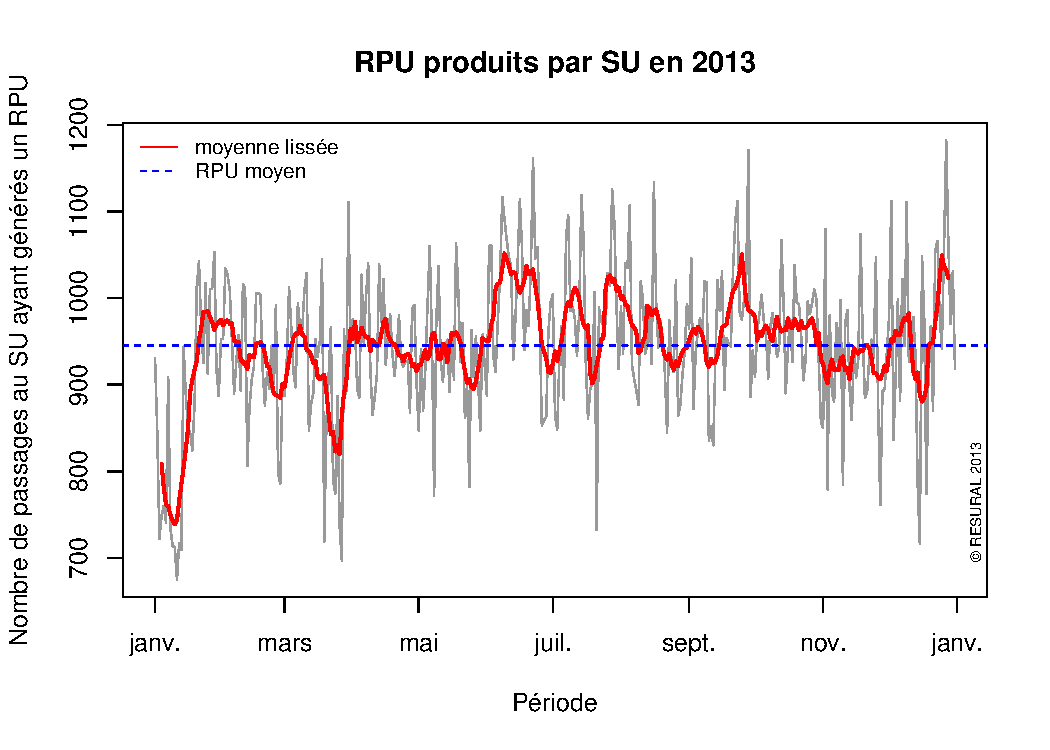
\includegraphics[width=\maxwidth]{figure/activite_plot-1} 

\end{knitrout}
\captionof{figure}{RPU produits par SU en 2013.}
\label{fig:activite_plot}
\end{center}

%\end{figure}

% Variante avec *xts*. Supprimé var n'apporte rien par rapport au précédent.

%\begin{figure}
% \begin{center}
% <<activite plot2, echo=FALSE, fig.height=5>>=
%   main <- paste0("Passages en SU en", anc)
%   x<-as.xts(z)
%  plot(x,ylab="Nb. de passages aux Urgences",main=main, xlab="Période")
% legend("topleft",legend="moyenne lissée",col="red",lty=1,cex=0.8,bty="n")
% lines(rollmean(xts(z),7),col="red",lwd=2)
% # moyenne générale
% abline(h=mean(a),col="blue")
%  mtext("© RESURAL 2013",cex=0.6,side=4,line=-1,adj=0.1)
% @
% \captionof{figure}{main.}
% \label{fig:activite_plot2}
% \end{center}
%\end{figure}

%------------------------------
\subsection*{En valeur absolue}
%------------------------------

% latex table generated in R 3.1.2 by xtable 1.7-1 package
% Sat Nov  8 20:44:56 2014
\begin{table}[ht]
\centering
\begin{tabular}{rcrr}
  \hline
 & Etablissement & RPU & SAE \\ 
  \hline
1 & 3Fr & 15 688 & 16 367 \\ 
  2 & Alk & 10 861 & 15 711 \\ 
  3 & Col & 64 758 & 64 116 \\ 
  4 & Dia & 29 469 &  \\ 
  5 & Geb & 15 103 & 21 644 \\ 
  6 & Hag & 34 414 & 43 441 \\ 
  7 & Hus & 37 018 & 103 446 \\ 
  8 & Mul & 56 195 & 61 266 \\ 
  9 & Odi & 25 963 & 26 025 \\ 
  10 & Sel & 29 534 & 29 699 \\ 
  11 & Wis & 12 646 & 12 545 \\ 
  12 & Sav & 12 424 & 27 736 \\ 
   \hline
\end{tabular}
\caption[Nombre de RPU par service d'urgence]{Nombre de RPU déclarés par service d'urgence en 2013 et données du fichier SAE} 
\label{fig:passage_su}
\end{table}


%\begin{figure}
\begin{center}
\begin{knitrout}
\definecolor{shadecolor}{rgb}{0.969, 0.969, 0.969}\color{fgcolor}
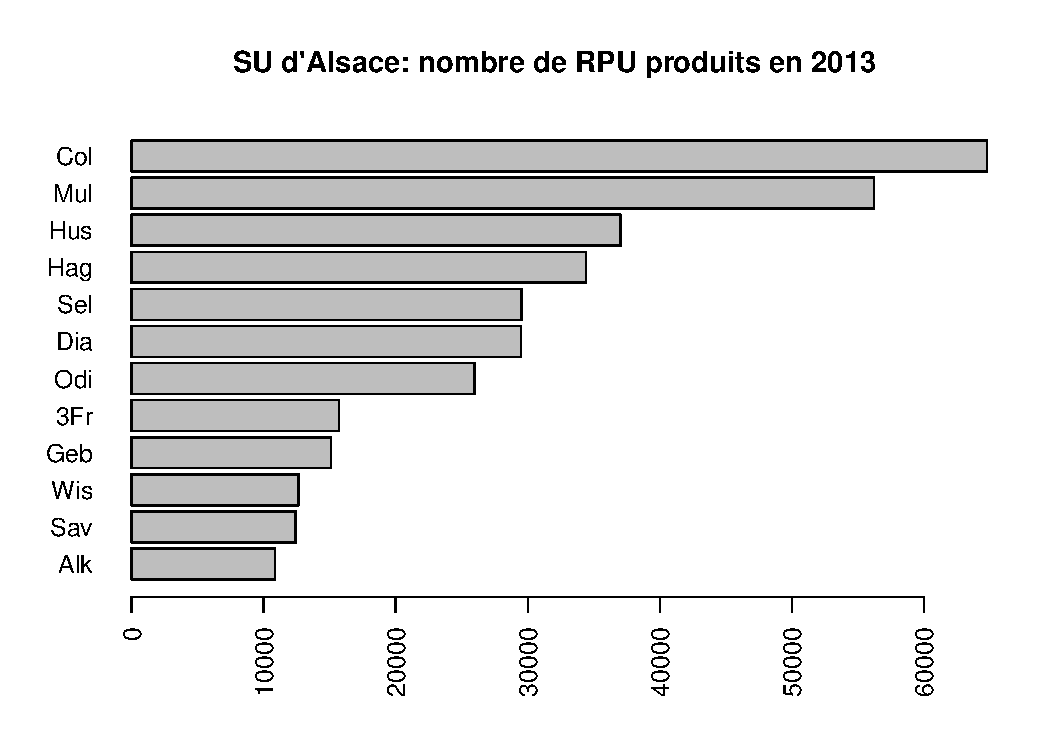
\includegraphics[width=\maxwidth]{figure/bplot_val_abs-1} 

\end{knitrout}
\captionof{figure}{SU d'Alsace: nombre de RPU produits en 2013.}
\label{fig:bplot_val_abs}
\end{center}
%\end{figure}

%------------------------------
\subsection*{En pourcentage}
%------------------------------



%\begin{figure}
\begin{center}
\begin{knitrout}
\definecolor{shadecolor}{rgb}{0.969, 0.969, 0.969}\color{fgcolor}
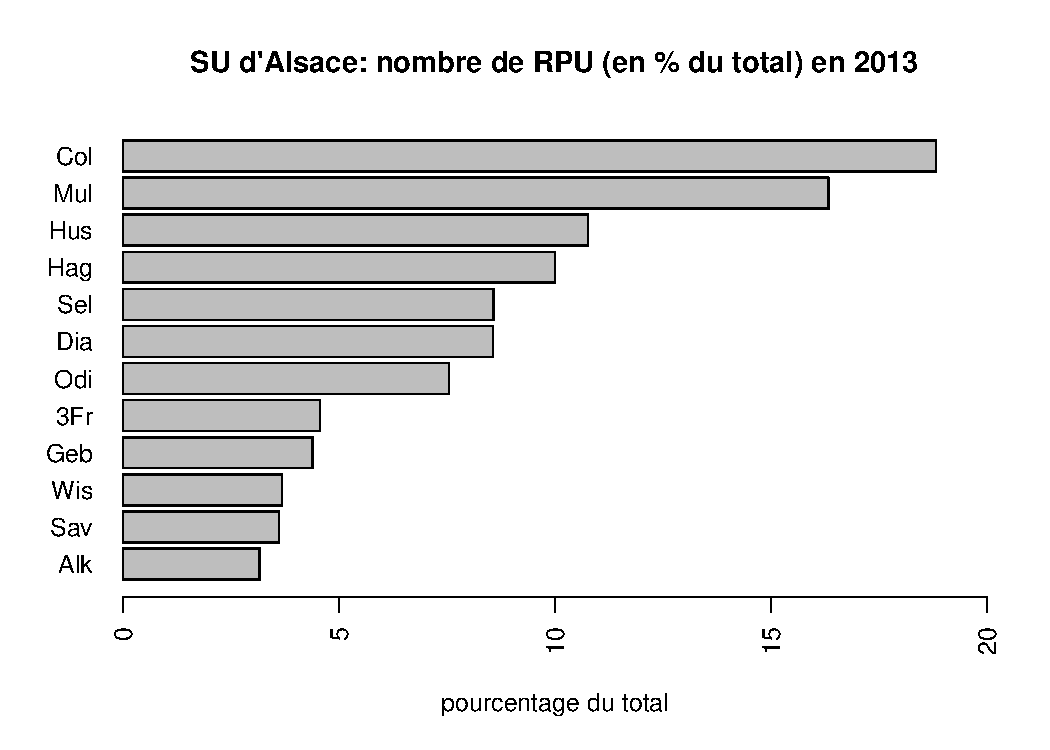
\includegraphics[width=\maxwidth]{figure/bp_en_pourcentage-1} 

\end{knitrout}
% \caption{main1.} # cette ligne fait bugger, pourquoi ?
\label{fig:bp_en_pourcentage}
\end{center}
%\end{figure}

%-----------------------------------------
\subsection*{Taux de recours aux urgences}
%-----------------------------------------


Le taux de recours aux urgences \index{taux de recours aux urgences} (TRU) \index{TRU} est défini comme le nombre total de passages aux urgences, rapporté à la population de la région (INSEE 1er janvier 2010). 

Le TRU 2013 estimé en Alsace à partir des RPU transmis est de 19\% et de 27\% en se basant sur les données SAE.

En Lorraine, ce taux est estimé à 23,45\% en 2010 (\cite{2,3}). 

%En supposant que la population alsacienne se comporte comme la population lorraine, le nombre de passages aux urgences devrait s'établir à tru_estime.

%------------------------------
\subsection*{Production mensuelle de RPU}
%------------------------------

% latex table generated in R 3.1.2 by xtable 1.7-1 package
% Sat Nov  8 20:44:56 2014
\begin{table}[ht]
\centering
\begin{tabular}{rr}
  \hline
 & RPU mensuels \\ 
  \hline
Jan & 26 858 \\ 
  Fev & 26 115 \\ 
  Mar & 28 312 \\ 
  Avr & 28 428 \\ 
  Mai & 27 899 \\ 
  Jun & 30 038 \\ 
  Jui & 30 103 \\ 
  Aou & 29 693 \\ 
  Sep & 29 190 \\ 
  Oct & 29 858 \\ 
  Nov & 27 657 \\ 
  Dec & 29 922 \\ 
   \hline
\end{tabular}
\caption{Ativité mensuelle en nombre de RPU en 2013. 28673 RPU en été produits en moyenne par mois en 2013} 
\end{table}


%\begin{figure}
\begin{center}
\begin{knitrout}
\definecolor{shadecolor}{rgb}{0.969, 0.969, 0.969}\color{fgcolor}
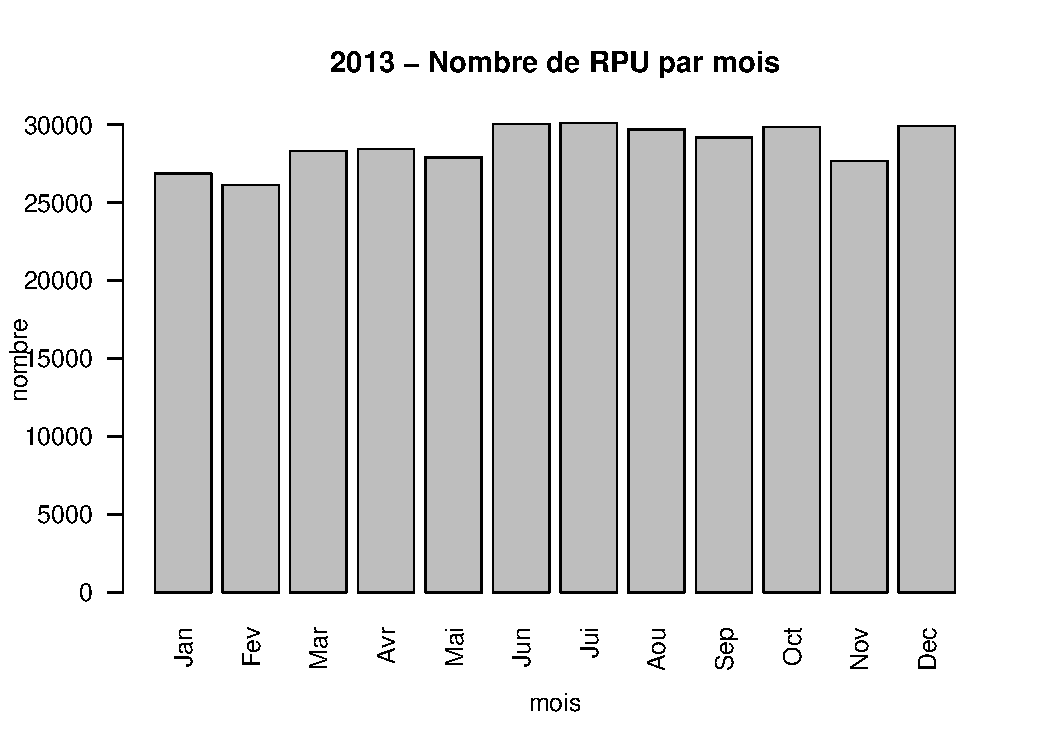
\includegraphics[width=\maxwidth]{figure/bp_parmois-1} 

\end{knitrout}
\captionof{figure}{2013 - Nombre de RPU par mois.}
\label{fig:bp_parmois}
\end{center}
%\end{figure}

Nombre de RPU par mois standards de 30 jours.

\begin{center}
\begin{knitrout}
\definecolor{shadecolor}{rgb}{0.969, 0.969, 0.969}\color{fgcolor}
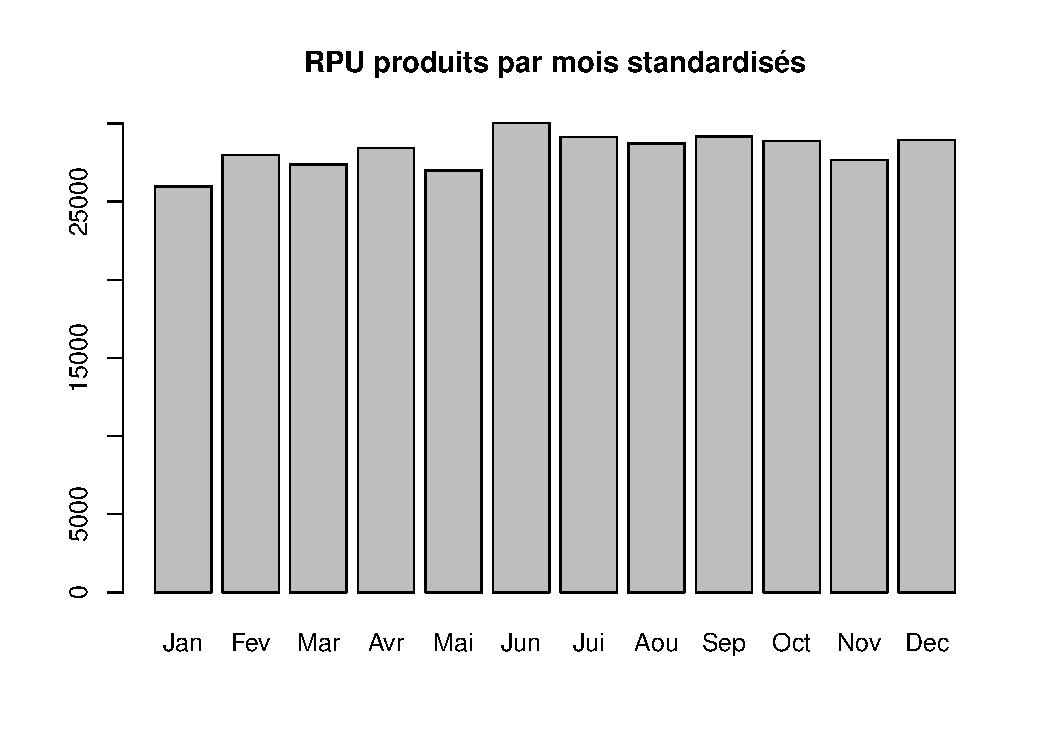
\includegraphics[width=\maxwidth]{figure/mois_nomalise-1} 

\end{knitrout}
\captionof{figure}{2013 - Nombre de RPU par mois standardisés de 30 jours.}
\label{fig:bp_parmois_std}
\end{center}

%---------------------------------
\subsection*{Activité par semaine}
%---------------------------------

% latex table generated in R 3.1.2 by xtable 1.7-1 package
% Sat Nov  8 20:44:57 2014
\begin{table}[ht]
\centering
\begin{tabular}{rrrrr}
  \hline
 & T1 & T2 & T3 & T4 \\ 
  \hline
1 & 4 752 & 5 170 & 6 242 & 6 885 \\ 
  2 & 6 823 & 6 645 & 6 530 & 6 451 \\ 
  3 & 6 305 & 6 712 & 6 478 & 6 060 \\ 
  4 & 6 232 & 6 698 & 6 632 & 6 667 \\ 
  5 & 6 538 & 6 462 & 6 628 & 6 720 \\ 
  6 & 6 314 & 5 615 & 7 116 & 7 213 \\ 
  7 & 7 193 & 6 569 & 6 566 & 7 083 \\ 
  8 & 6 391 & 7 069 & 6 995 & 6 726 \\ 
  9 & 6 861 & 6 502 & 6 568 & 6 768 \\ 
  10 & 6 474 & 6 891 & 7 152 & 6 727 \\ 
  11 & 6 760 & 6 763 & 6 757 & 6 500 \\ 
  12 & 6 427 & 6 489 & 6 620 & 6 390 \\ 
  13 & 6 705 & 6 411 & 6 619 & 7 260 \\ 
   \hline
\end{tabular}
\caption[Activité par semaine]{Activité des services d'urgence en nombre de RPU par semaine en 2013} 
\label{act_sem}
\end{table}


%\begin{figure}
\begin{center}
\begin{knitrout}
\definecolor{shadecolor}{rgb}{0.969, 0.969, 0.969}\color{fgcolor}
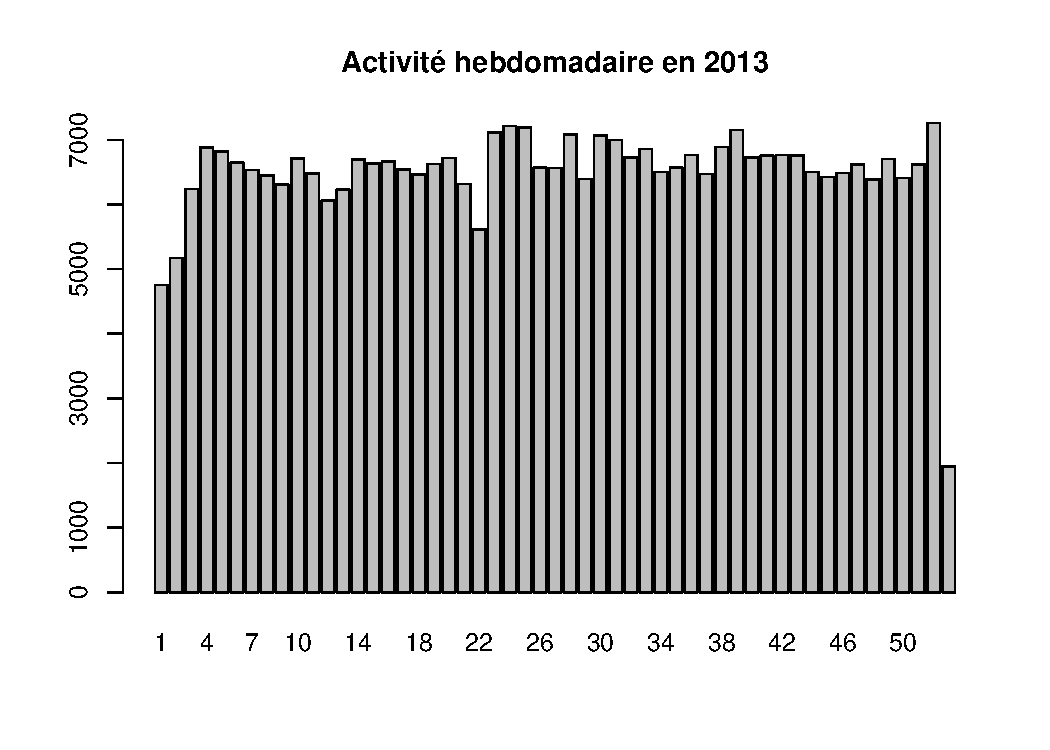
\includegraphics[width=\maxwidth]{figure/bp_act_sem-1} 

\end{knitrout}
\captionof{figure}{Activité hebdomadaire en 2013.}
\label{fig:act_sem}
\end{center}
%\end{figure}

%--------------------------------------------
\subsection*{Activité par jour de la semaine}
%--------------------------------------------

\begin{table}[ht]
\centering
\begin{tabular}{rr}
  \hline
 & RPU selon le jour \\ 
  \hline
Lun & 52 804 \\ 
  Mar & 48 522 \\ 
  Mer & 46 335 \\ 
  Jeu & 48 142 \\ 
  Ven & 47 782 \\ 
  Sam & 50 368 \\ 
  Dim & 50 120 \\ 
   \hline
\end{tabular}
\caption[RPU par jour de semaine]{Ativité selon le jour de la semaine en nombre de RPU en 2013} 
\end{table}


\begin{center}
\begin{knitrout}
\definecolor{shadecolor}{rgb}{0.969, 0.969, 0.969}\color{fgcolor}
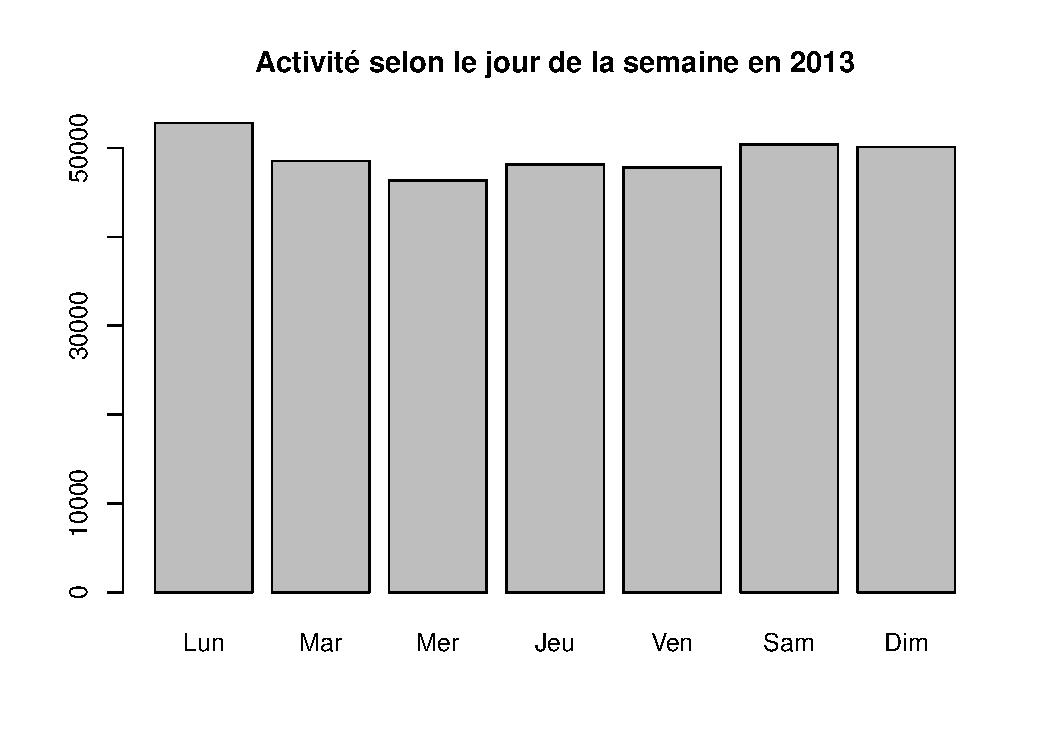
\includegraphics[width=\maxwidth]{figure/bp_activite_semaine-1} 

\end{knitrout}
\captionof{figure}{Activité selon le jour de la semaine en 2013. Le lundi est le jour où la fréquentation des urgences est la plus importante. C'est aussi le jour des admission réglée dans les services. Le lundi est un jour à risque de tension hospitalière de type organisationnelle.}
\label{fig:activite_semaine}
\end{center}

%------------------------------
\subsection*{Activité horaire}
%------------------------------



\begin{center}
\begin{knitrout}
\definecolor{shadecolor}{rgb}{0.969, 0.969, 0.969}\color{fgcolor}
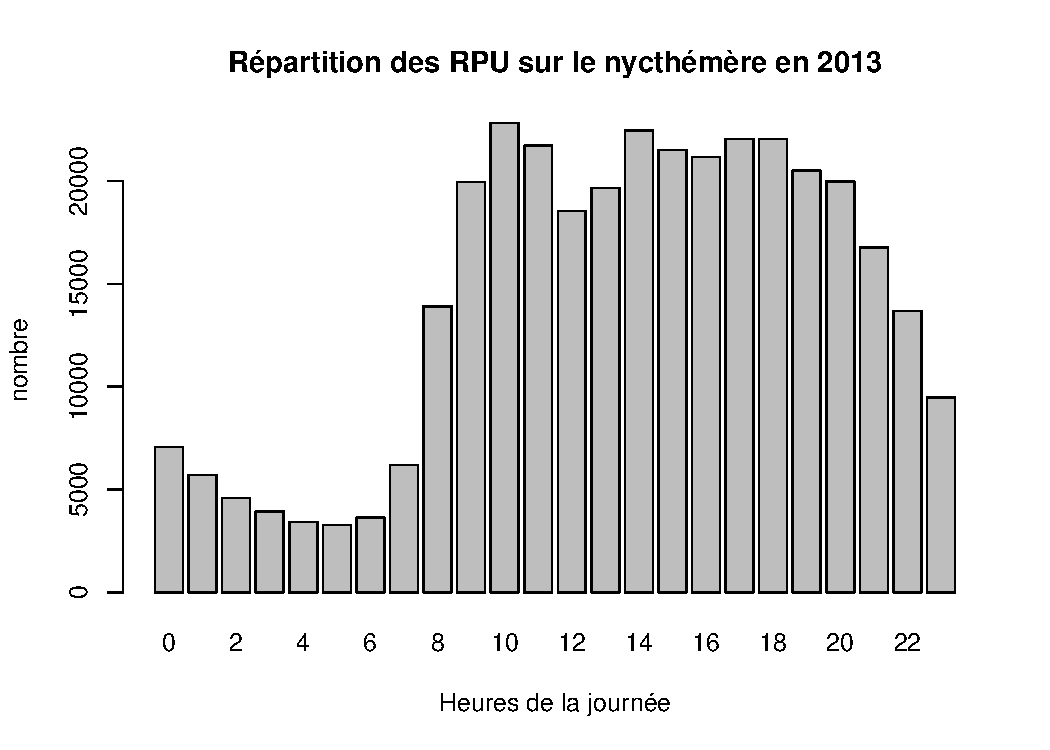
\includegraphics[width=\maxwidth]{figure/bp_activite_heure-1} 

\end{knitrout}
\captionof{figure}{Répartition des RPU sur le nycthémère en 2013.}
\label{fig:activite_heure}
\end{center}

Le profil du graphe est identique à celui de l'activité des SAMU. Urgences intra-hospitalières et extra-hospitalières ont des profils d'ativité identiques rendant difficile la mutualisation des activités.

%----------------------------------
\subsection{Typologie des passages \protect\footnote{attente.Rmd}} 
% si on met une note dans un titre de section, il faut la protéger avec \protect. Source: http://www.tuteurs.ens.fr/logiciels/latex/footnote.html
%----------------------------------

\index{passages!typologie}

%---------------------------------
\subsubsection*{Tous les passages}
%---------------------------------

% dessinne les courbes d'entrée et de sortie sur 24h.
% une fonction générique serait utile.
 
 \begin{center}
\begin{knitrout}
\definecolor{shadecolor}{rgb}{0.969, 0.969, 0.969}\color{fgcolor}
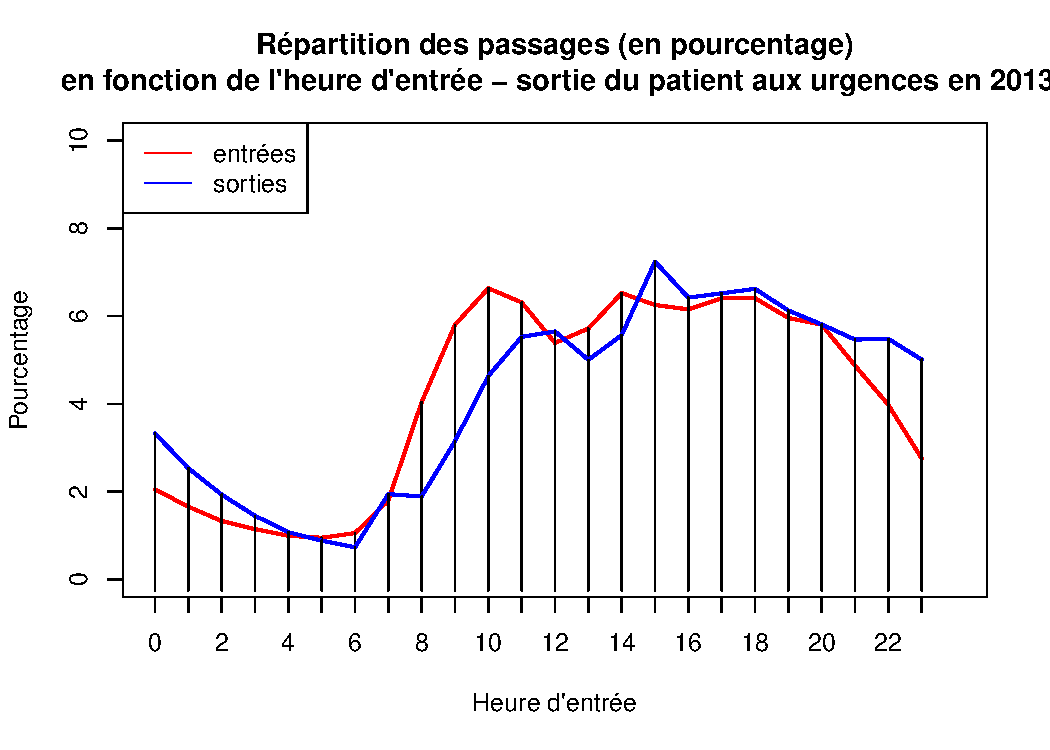
\includegraphics[width=\maxwidth]{figure/sau_arrive_depart-1} 

\end{knitrout}
\captionof{figure}{Répartition des passages (en pourcentage)
 en fonction de l'heure d'entrée - sortie du patient aux urgences en 2013.}
\label{fig:sau_arrive_depart}
\end{center}

 
%---------------------------------------------
\subsubsection*{Passages Diurnes - Nocturnes}
%---------------------------------------------

\begin{itemize}
  \item diurne: 8h - 19h59   
  
  \item nocturne: 20h - 7h59
\end{itemize}



\index{admission diurne}
\index{Recours nocturne}
\index{sortie diurne}

\begin{boxedminipage}{10cm}
\begin{itemize}
  \item Admission diurne: 72 \%
  \item Recours nocturne: 28 \%
  \item Sortie diurne:    64 \%
  \item Ratio entrée/sortie diurne: 1.2
  \item Ratio entrée/sortie nocturne: 0.87
\end{itemize}
\end{boxedminipage}

%-----------------------------------------
\subsubsection*{Entrée - sorties adultes}
%-----------------------------------------

\begin{center}
\begin{knitrout}
\definecolor{shadecolor}{rgb}{0.969, 0.969, 0.969}\color{fgcolor}
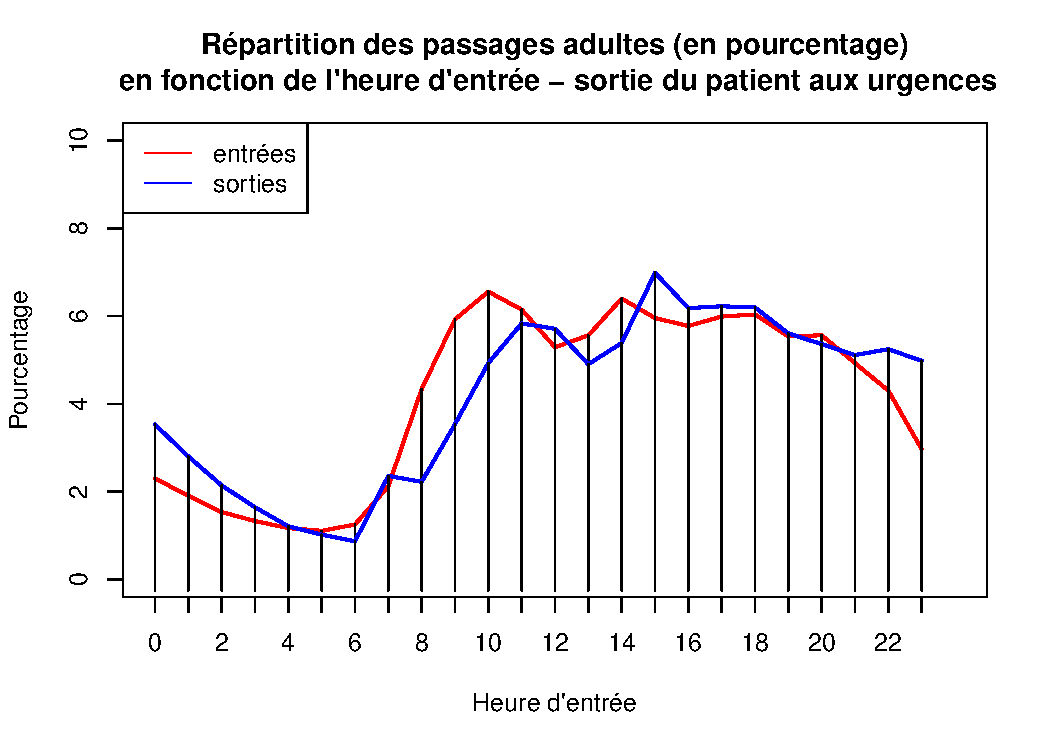
\includegraphics[width=\maxwidth]{figure/es_adultes-1} 

\end{knitrout}
\captionof{figure}{Répartition des passages adultes (en pourcentage).}
\label{fig:es_adultes}
\end{center}

Pour la pédiatrie (pp.\pageref{chap_pediatrie}) et la gériatrie (pp.\pageref{chap_geriatrie}), on se reportera aux chapitres correspondants.

%----------------------------------
\subsubsection*{Semaine - Week-end}
%----------------------------------

\index{Entrée-sorties du weekend}

\begin{itemize}
  \item semaine: du lundi 8h au vendredi 19h59
  \item week-end: du vendredi 20h au lundi 7h59
\end{itemize}




% # graphe entrées semaine/we

\begin{center}
\begin{knitrout}
\definecolor{shadecolor}{rgb}{0.969, 0.969, 0.969}\color{fgcolor}
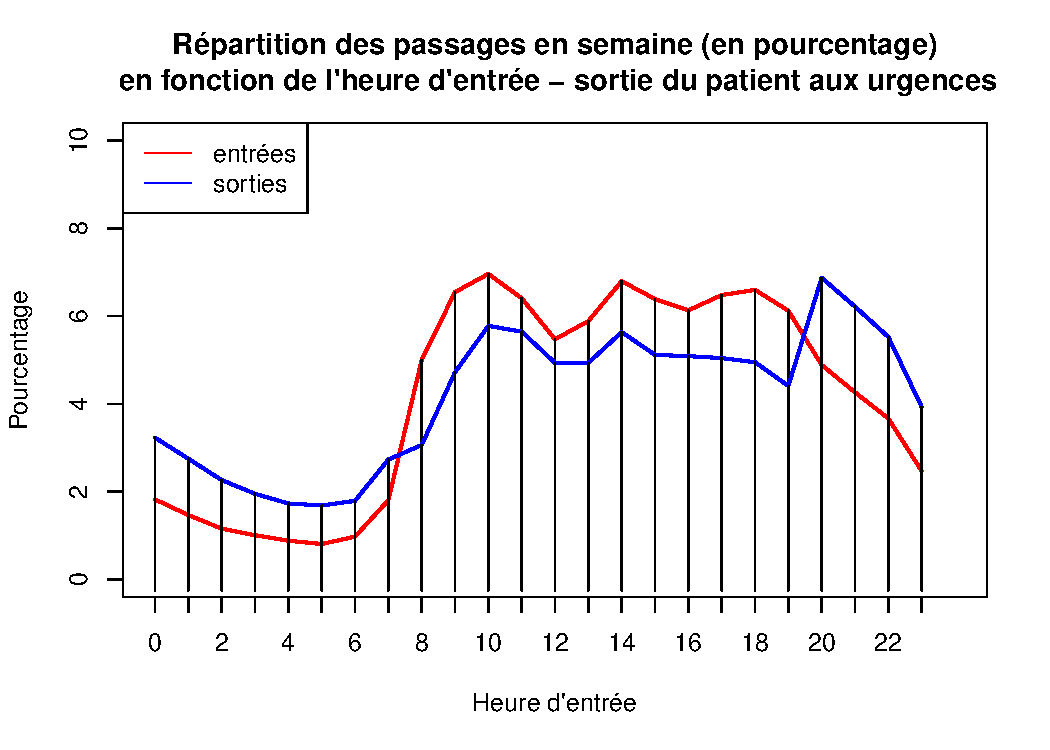
\includegraphics[width=\maxwidth]{figure/graphe_es_we-1} 

\end{knitrout}
\captionof{figure}{"Répartition des passages en semaine (en pourcentage)\\ en fonction de l'heure d'entrée - sortie du patient aux urgences"}
\label{fig:graphe_es_we} %
\end{center}


% graphe des sorties semaine/we

\begin{center}
\begin{knitrout}
\definecolor{shadecolor}{rgb}{0.969, 0.969, 0.969}\color{fgcolor}
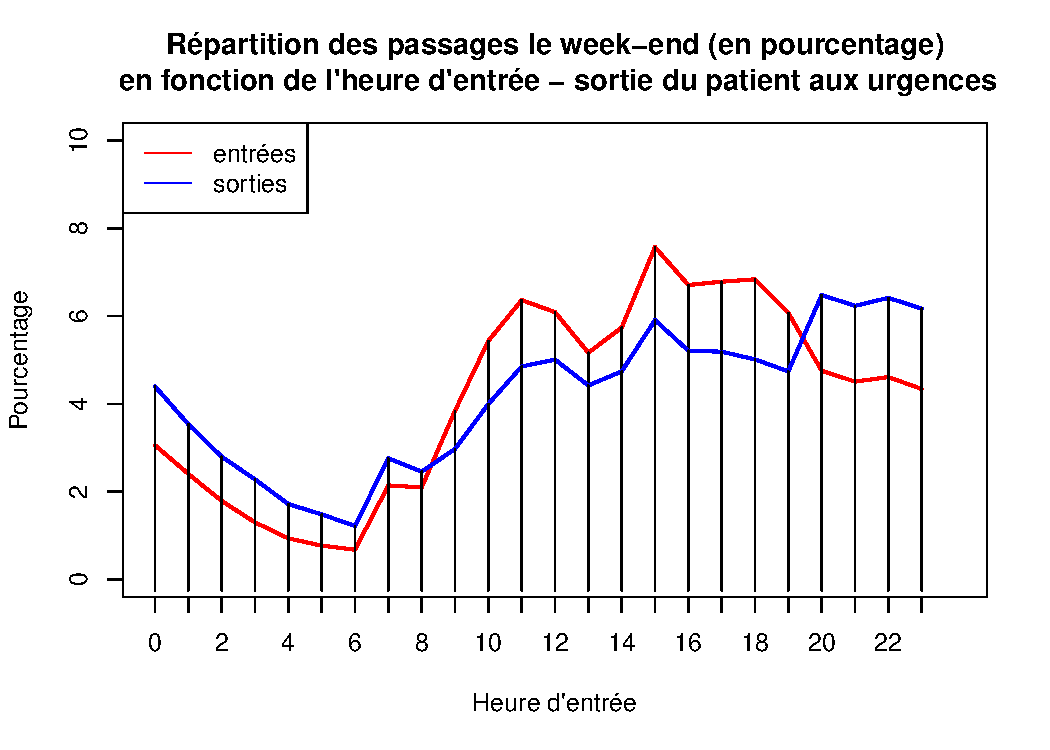
\includegraphics[width=\maxwidth]{figure/graphe2_es_we-1} 

\end{knitrout}
\captionof{figure}{"Répartition des passages en semaine (en pourcentage)\\ en fonction de l'heure d'entrée - sortie du patient aux urgences"}
\label{fig:graphe2_es_we} %
\end{center}

\begin{boxedminipage}{10cm}
\begin{itemize}
  \item entrées en semaine 136 833
  \item entrées le weekend: 70 734
  \item pourcentage des entrées en semaine: 66 \%
  \item \textbf{Part d'activité de week-end: 34 \%}
  \item sorties en semaine 141 749
  \item sorties le weekend: 85 986
  \item pourcentage de sorties en semaine: 62
\end{itemize}
\end{boxedminipage}

%------------------------------------------------
\subsubsection*{Entrées sorties des hospitalisés}
%------------------------------------------------

\index{Entrées sorties des hospitalisés}

\begin{center}
\begin{knitrout}
\definecolor{shadecolor}{rgb}{0.969, 0.969, 0.969}\color{fgcolor}
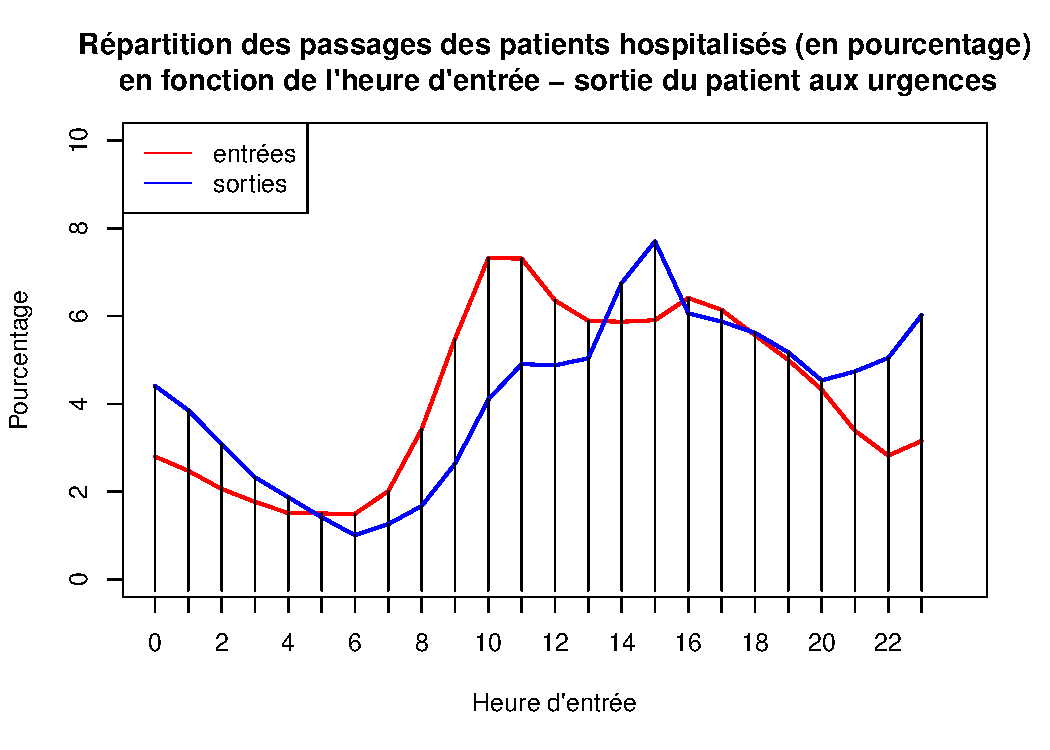
\includegraphics[width=\maxwidth]{figure/es_hospitalise-1} 

\end{knitrout}
\captionof{figure}{Répartition des passages des patients hospitalisés (en pourcentage)
 en fonction de l'heure d'entrée - sortie du patient aux urgences.}\label{fig:es_hospitalise}%
\end{center}

%------------------------------------------------------
\subsubsection*{Entrées sorties des retours à domicile}
%------------------------------------------------------

\index{Entrées sorties des retours à domicile}

\begin{center}

\begin{knitrout}
\definecolor{shadecolor}{rgb}{0.969, 0.969, 0.969}\color{fgcolor}
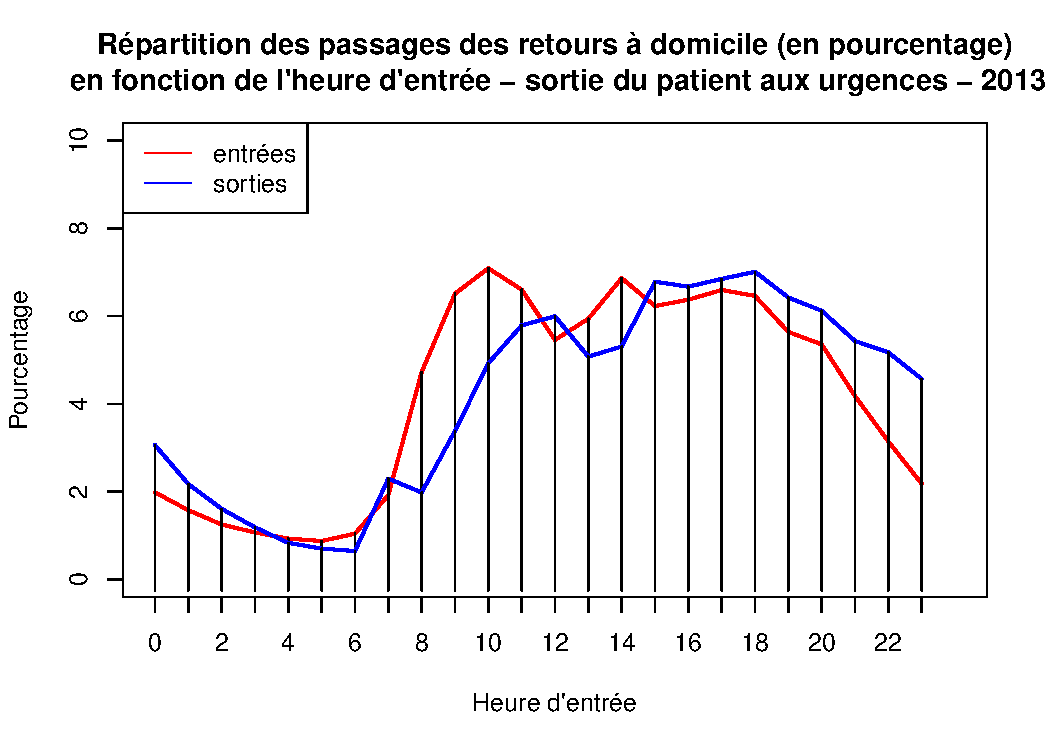
\includegraphics[width=\maxwidth]{figure/es_dom-1} 

\end{knitrout}
\captionof{figure}{Répartition des passages des retours à domicile (en pourcentage)
 en fonction de l'heure d'entrée - sortie du patient aux urgences - 2013.}\label{fig:es_dom}%
\end{center}

\section{Passages aux urgences}

% test2.Rnw

L'activité horaire des services d'urgence en Alsace est totalement superposable à celle de l'ensemble des SU (figure \ref{passage:als} page \pageref{passage:als}). L'activité diminue fortement en nuit profonde à partir de une heure du matin pour redémarrer vers 9 heures et s'intensifier progressivement en matinée. Après un premier pic en fin de matinée, la croissance reprend pour culminer vers 19 heures, puis décroître lentement jusqu'en fin de soirée.

Ce phénomène cyclique se répète tous les jours selon un profil immuable. La projection de ces données sur un graphique en radar représentant les 24 tranches horaires (figure \ref{radar:als} page \pageref{radar:als}) montre qu'il existe trois pics d'égale amplitude à 11, 15 et 19 heures. Ce point mérite d'être analysé car s'il se confirme, cela pourrait indiquer que le pointage de 11 heures permet d'avoir une prévision sur l'intensité de la fréquentation avant la garde du soir. On peut en rapprocher le fait que la médiane des passages se situe vers 14h, c'est à dire qu'au pointage de 15 heures on peut évaluer la quantité totale de patients qui vont se présenter dans les heures qui viennent.

%----------------------------------------------------------------------------- Summary
Résumé des horaires de passage aux urgences: les données figurent dans le tableau \ref{tab:24} page \pageref{tab:24}.
% latex table generated in R 3.1.2 by xtable 1.7-1 package
% Sat Nov  8 20:45:01 2014
\begin{table}[ht]
\centering
\begin{tabular}{rrrrrrrrrrr}
  \hline
 & n & Min & Q25 & Moyenne & E-type & Médiane & Q75 & Max & Na & \%Na \\ 
  \hline
 & 344 073,00 & 0,00 & 10,00 & 13,90 & 5,60 & 14,00 & 18,00 & 23,00 & 0,00 & 0,00 \\ 
   \hline
\end{tabular}
\caption[Horaires de passage]{Résumé des horaires de passage aux urgences en 2013. A 18 heures, 75 p.cent des RPU de la journée sont enregistés.} 
\label{tab:24}
\end{table}


% \input{../blah.gen}
%---------------------------------------------------------------------- HISTOGRAMME

%\begin{figure}
\begin{center}
\begin{knitrout}
\definecolor{shadecolor}{rgb}{0.969, 0.969, 0.969}\color{fgcolor}
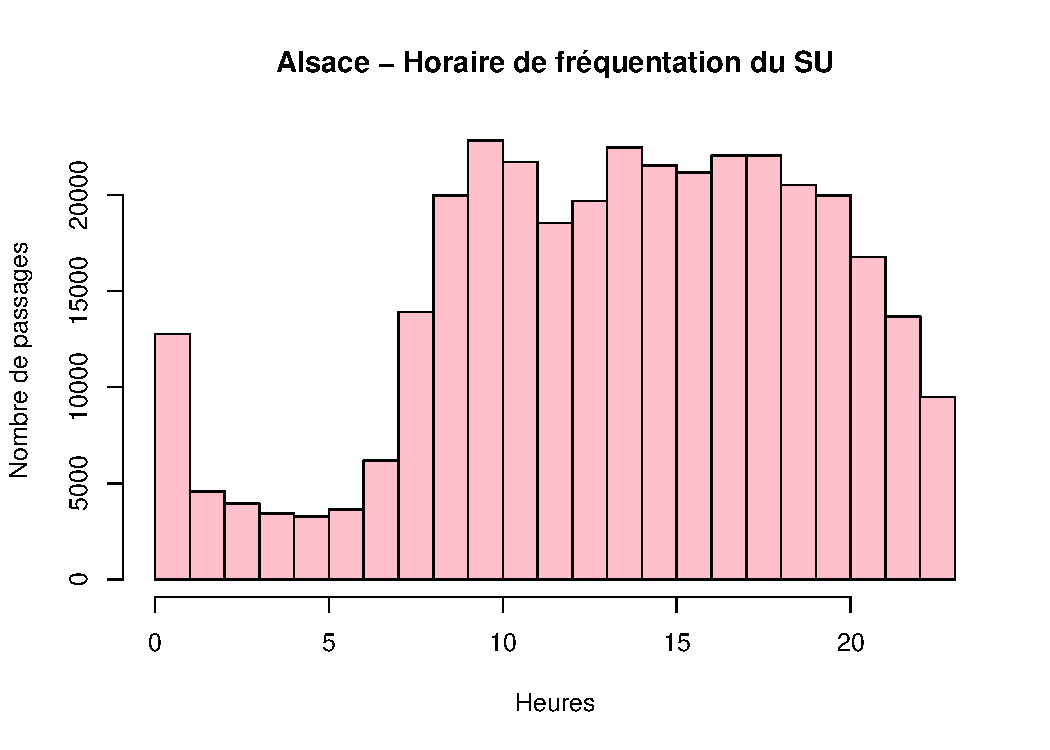
\includegraphics[width=\maxwidth]{figure/test23-1} 

\end{knitrout}
\captionof{figure}{Horaires d'arrivée aux urgences en Alsace 2013}
\label{passage:als}
\end{center}

%\end{figure}
%---------------------------------------------------------------------------- RADAR 1

%\begin{figure}
\begin{center}
\begin{knitrout}
\definecolor{shadecolor}{rgb}{0.969, 0.969, 0.969}\color{fgcolor}
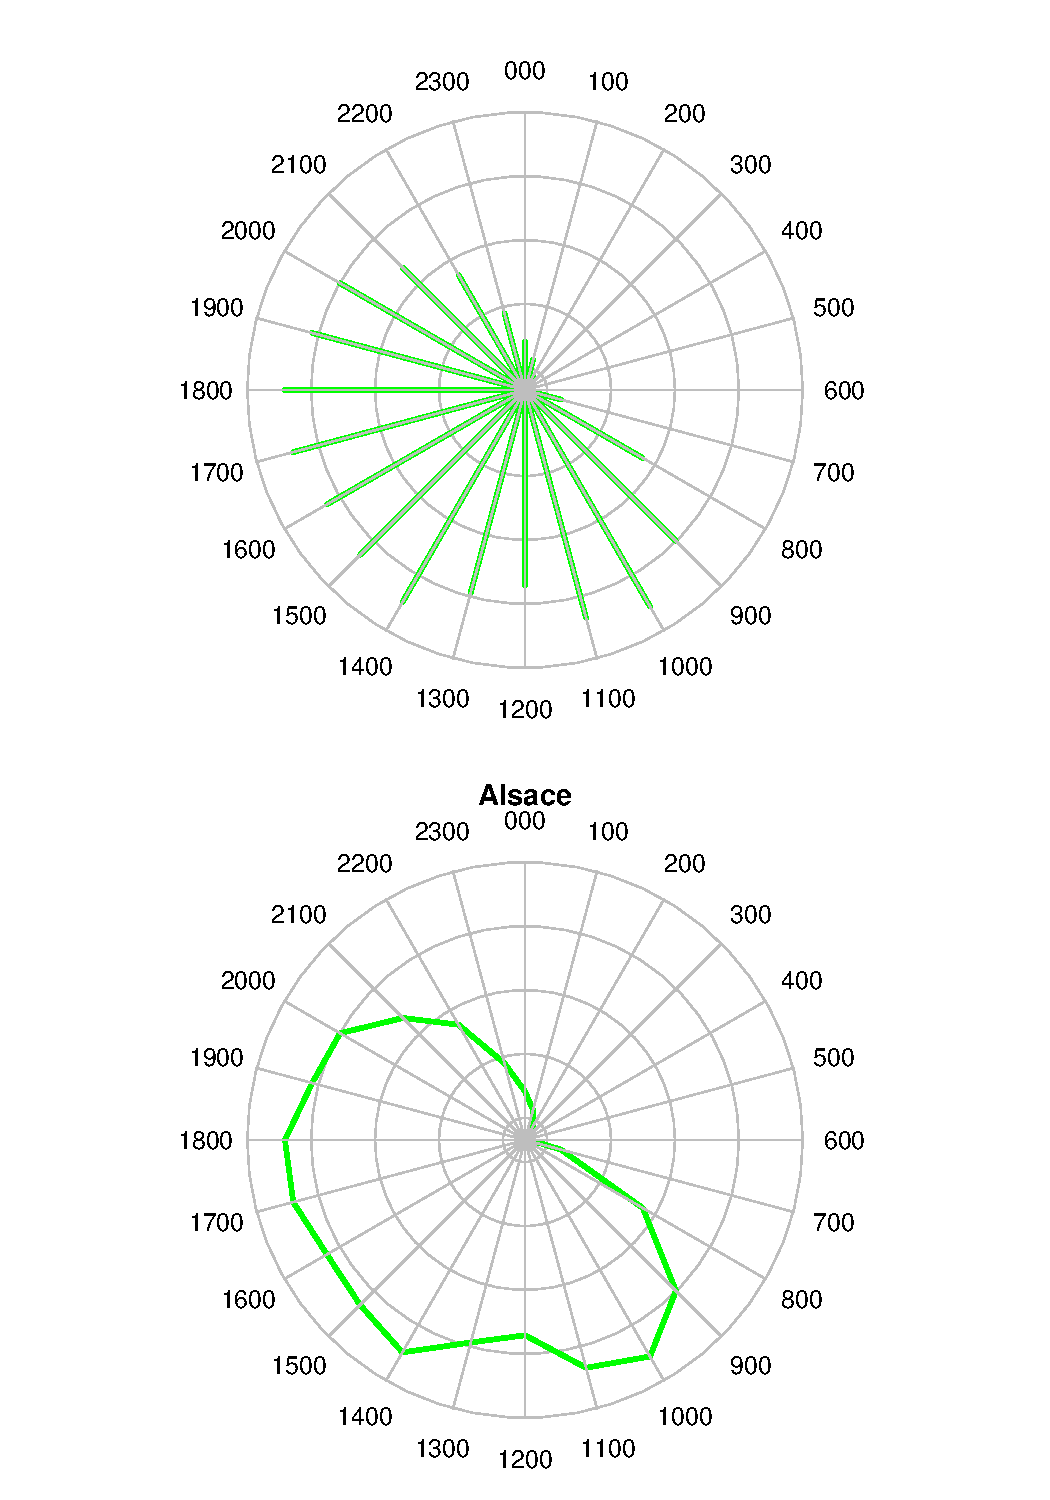
\includegraphics[width=\maxwidth]{figure/test25-1} 

\end{knitrout}
\captionof{figure}{Horaires d'arrivée aux urgences en Alsace 2013}
\label{radar:als}
\end{center}

%\end{figure}

%---------------------------------------------------------Radar HUS

% \begin{center}
%   <<test2, echo=FALSE,fig = TRUE,fig.height=5,warning=FALSE>>=
%     passages("Hus","HUS",sens=3)
%     @
% \captionof{figure}{HUS: répartition des arrivées et départs aux urgences}
% \label{passage:hus}
% \end{center}

%---------------------------------------------------------Radar Colmar
%\begin{figure}
\begin{center}
\begin{knitrout}
\definecolor{shadecolor}{rgb}{0.969, 0.969, 0.969}\color{fgcolor}
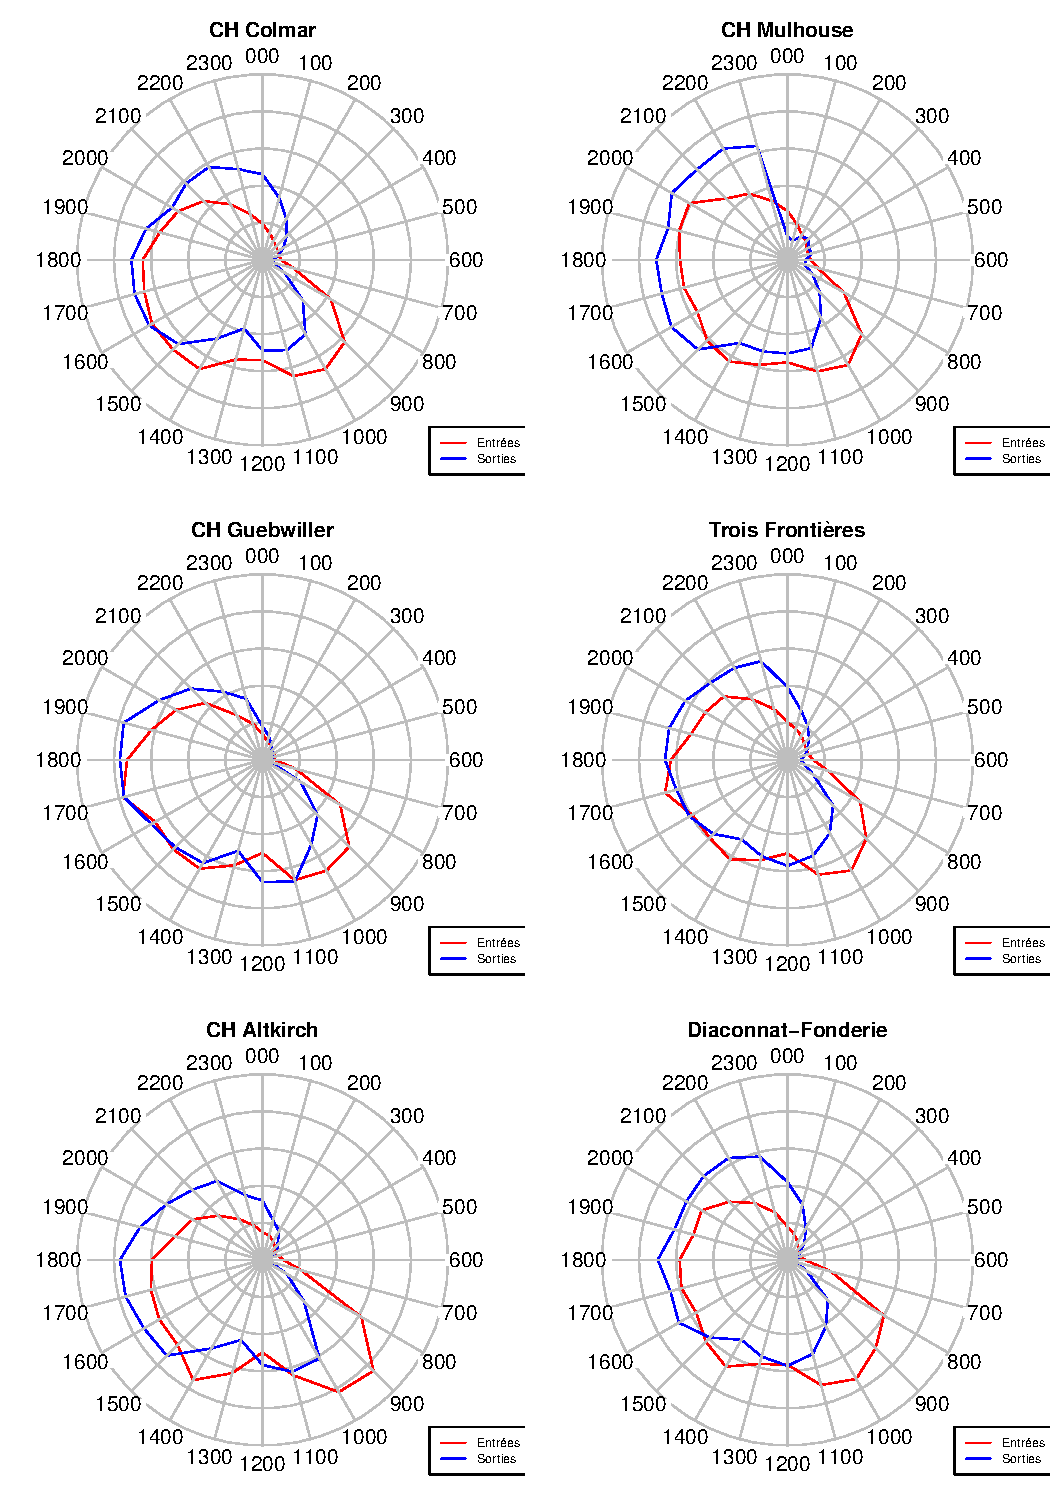
\includegraphics[width=\maxwidth]{figure/test26-1} 

\end{knitrout}
\captionof{figure}{Secteurs 3 et 4: répartition des arrivées et départs aux urgences}
\label{passage:col}
\end{center}

%\end{figure}

%\begin{figure}
\begin{center}
\begin{knitrout}
\definecolor{shadecolor}{rgb}{0.969, 0.969, 0.969}\color{fgcolor}
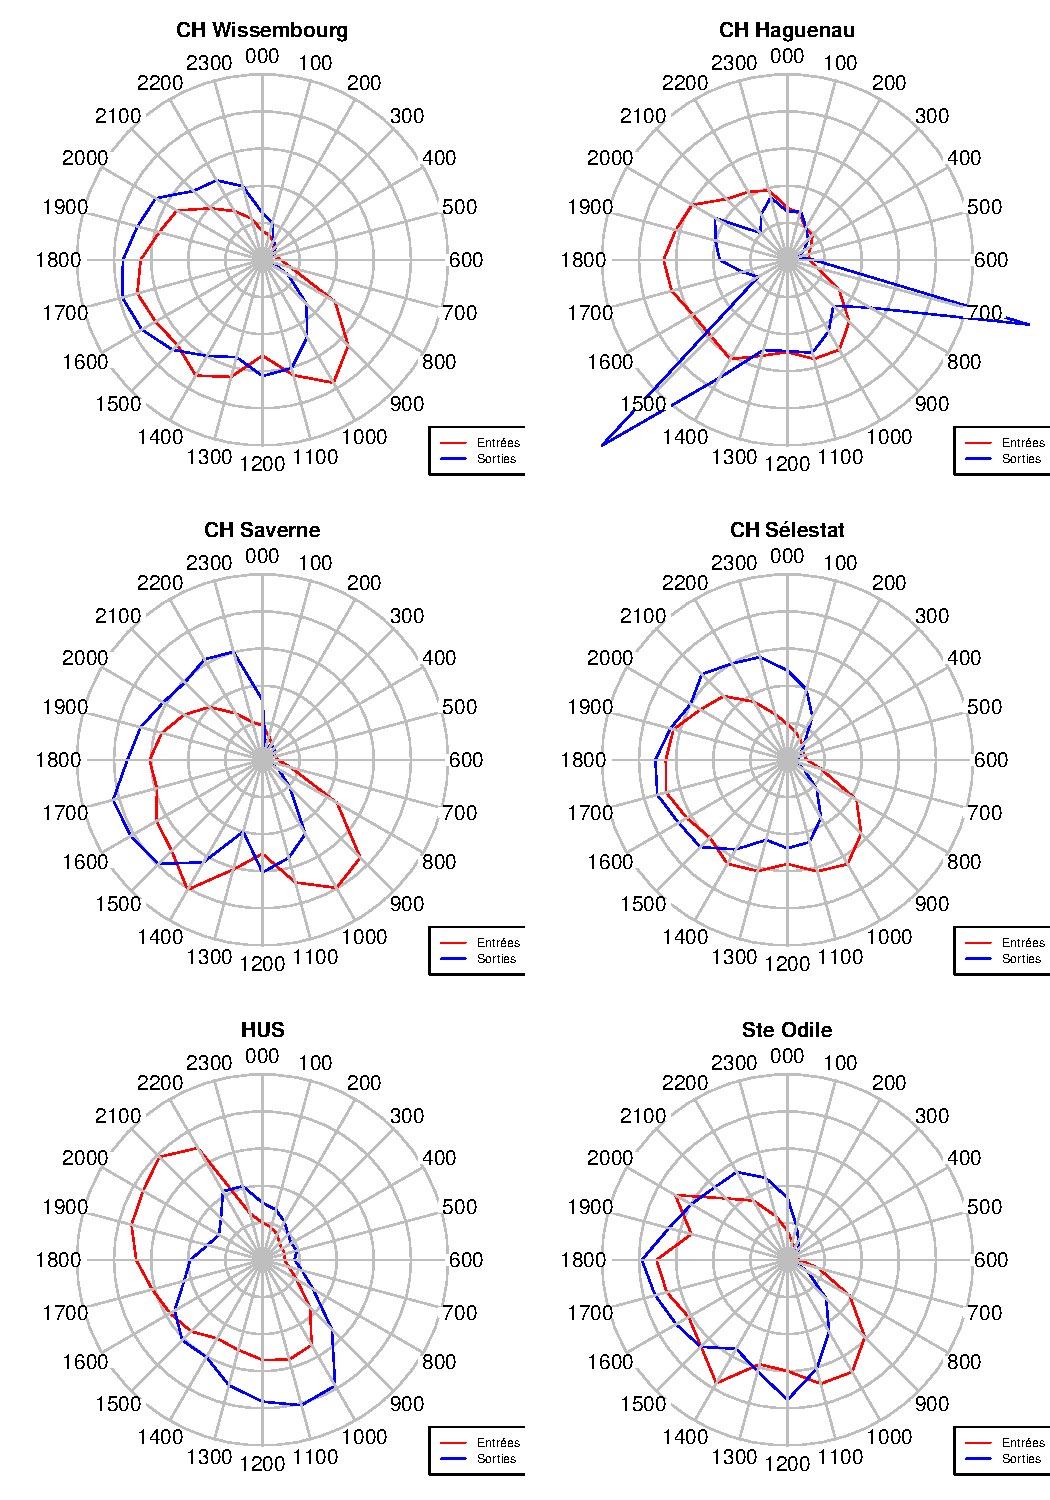
\includegraphics[width=\maxwidth]{figure/test27-1} 

\end{knitrout}
\captionof{figure}{Secteurs 1 et 2: répartition des arrivées et départs aux urgences}
\label{passage:secteur12}
\end{center}

%\end{figure}


\section{Passages en fonction de l'âge}

% tranche-age.Rnw

\subsection*{Pyramide des âges en Alsace}
%-------------------------------------------
\index{Pyramide des âges!Alsace}
\index{Age}
\index{Tranches d'age}

% ce paragraphe utilise intensivement le dessin des pyramides: utiliser la syntaxe pp <- pyramid.plot() qui provoque le dessin de la pyramide tandis que les valeurs de retours sont stockées dans pp et n'apparaissent pas à l'impression.

% latex table generated in R 3.1.2 by xtable 1.7-1 package
% Sat Nov  8 20:45:04 2014
\begin{table}[ht]
\centering
\begin{tabular}{rlrrr}
  \hline
 & X & Hommes & Femmes & Ensemble \\ 
  \hline
1 & Moins de 5 ans & 55 914 & 53 240 & 109 154 \\ 
  2 & 5 à 9 ans & 56 840 & 54 235 & 111 075 \\ 
  3 & 10 à 14 ans & 56 710 & 54 357 & 111 067 \\ 
  4 & 15 à 19 ans & 58 843 & 56 599 & 115 441 \\ 
  5 & 20 à 24 ans & 58 106 & 59 818 & 117 924 \\ 
  6 & 25 à 29 ans & 57 879 & 59 193 & 117 072 \\ 
  7 & 30 à 34 ans & 57 264 & 57 915 & 115 179 \\ 
  8 & 35 à 39 ans & 65 126 & 65 588 & 130 714 \\ 
  9 & 40 à 44 ans & 68 519 & 67 953 & 136 472 \\ 
  10 & 45 à 49 ans & 67 881 & 68 439 & 136 319 \\ 
  11 & 50 à 54 ans & 64 389 & 65 566 & 129 956 \\ 
  12 & 55 à 59 ans & 61 926 & 62 187 & 124 114 \\ 
  13 & 60 à 64 ans & 50 598 & 50 280 & 100 878 \\ 
  14 & 65 à 69 ans & 36 682 & 38 515 & 75 197 \\ 
  15 & 70 à 74 ans & 31 586 & 37 465 & 69 051 \\ 
  16 & 75 à 79 ans & 25 776 & 36 071 & 61 847 \\ 
  17 & 80 à 84 ans & 16 584 & 29 995 & 46 579 \\ 
  18 & 85 à 89 ans & 8 009 & 19 326 & 27 336 \\ 
  19 & 90 à 94 ans & 1 815 & 5 825 & 7 640 \\ 
  20 & 95 à 99 ans & 430 & 1 883 & 2 313 \\ 
  21 & 100 ans ou plus &  42 & 316 & 358 \\ 
   \hline
\end{tabular}
\caption[Population d'Alsace en 2010]{Population d'Alsace en 2010 (source INSEE - Population légale 2010)} 
\label{tab:pop_insee}
\end{table}


La répartition de la population alsacienne par tranche d'âge est fournie par l'INSEE (table \ref{tab:pop_insee} page \pageref{tab:pop_insee}). La somme des valeurs donne un chiffre de 1 845 685 personnes dans la région Alsace en 2010.

%\begin{figure}
\begin{center}
\begin{knitrout}
\definecolor{shadecolor}{rgb}{0.969, 0.969, 0.969}\color{fgcolor}
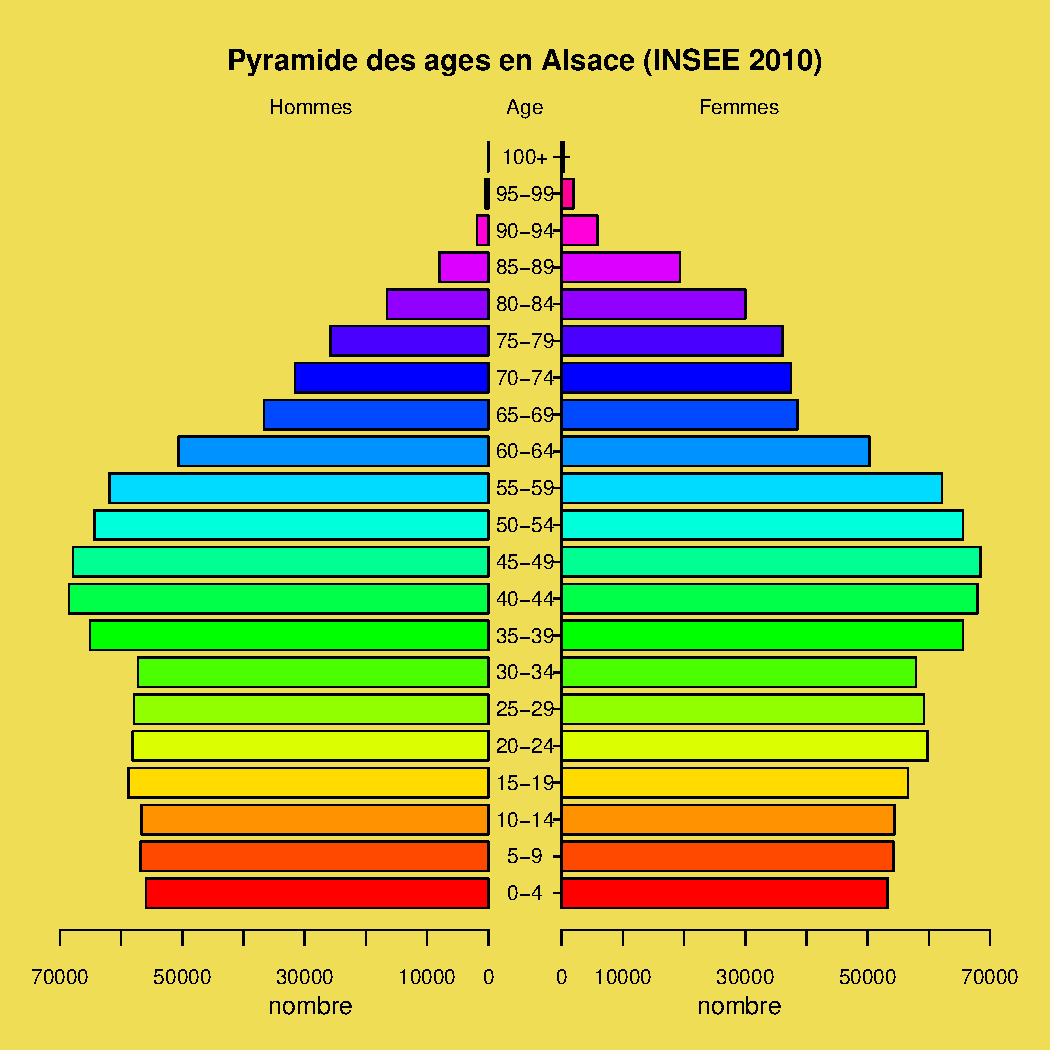
\includegraphics[width=\maxwidth]{figure/pyramide_graphe-1} 

\end{knitrout}
\captionof{figure}{Pyramides des âges en Alsace (source INSEE)}
\label{fig:pyr_age_insee}
\end{center}

%\end{figure}

%\begin{figure}
\begin{center}
\begin{knitrout}
\definecolor{shadecolor}{rgb}{0.969, 0.969, 0.969}\color{fgcolor}
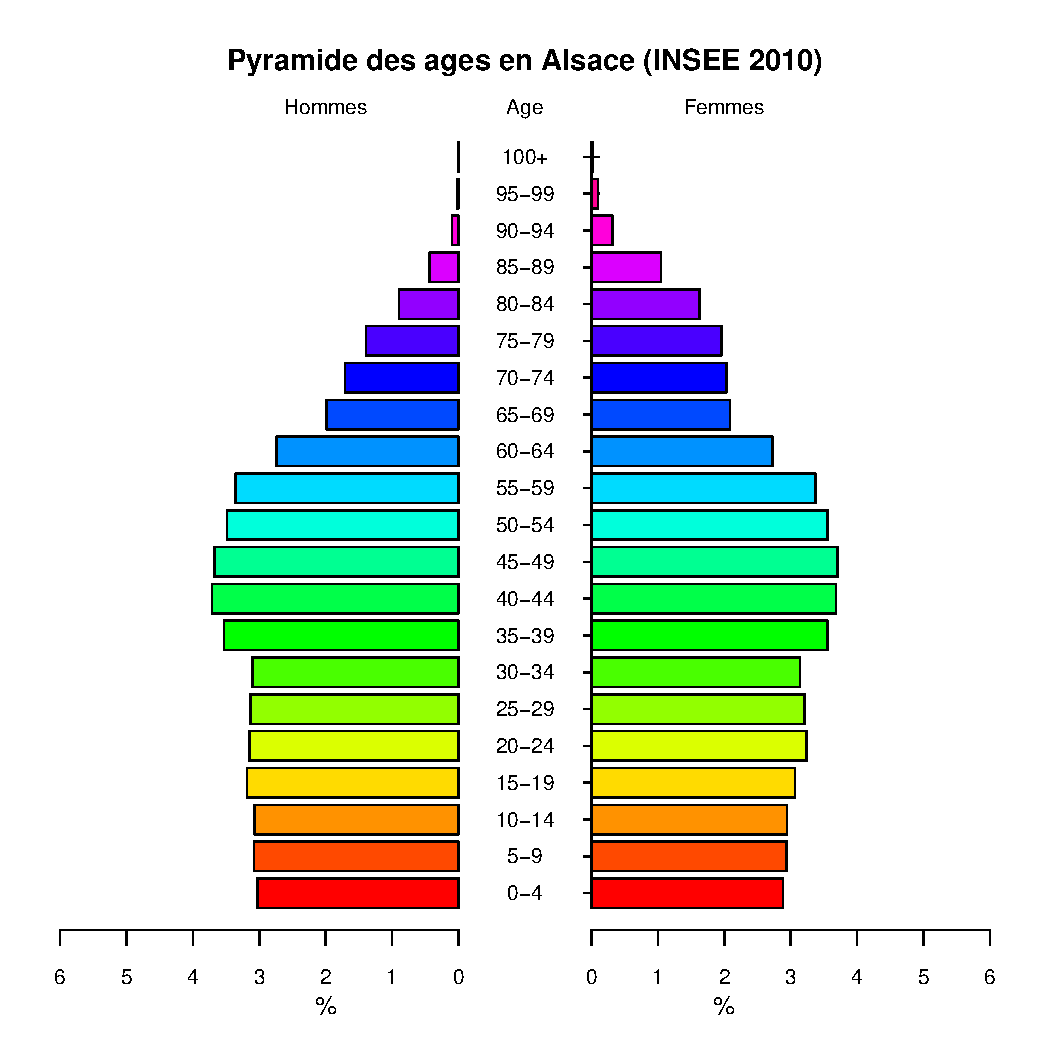
\includegraphics[width=\maxwidth]{figure/pyramide_graphe2-1} 

\end{knitrout}
\captionof{figure}{Pyramides des âges en Alsace (source INSEE)}
\label{fig:pyr_age_inseep100}
\end{center}

%\end{figure}



\subsection*{Analyse de la variable AGE}
%------------------------------------------

Les RPU utilisent la date de naissance. L'âge est calculé en soustrayant l’année de naissance de l'année courante (âge atteint dans l'année).

% la doc de ce chapitre est dans tranche_age.Rmd




Les âges répertoriés vont de moins de 1 an à 113 ans. L'âge moyen est de 40 ans (médiane 38 ans). L'âge moyen des hommes est de 38 ans et celui des femmes de 43 ans.

Il existe plusieurs façons de former des tranches d'âges.

% ### Age 1
%----------

% latex table generated in R 3.1.2 by xtable 1.7-1 package
% Sat Nov  8 20:45:05 2014
\begin{table}[ht]
\centering
\begin{tabular}{lrr}
  \hline
Tranches d'age & RPU & \%  \\ 
  \hline
Moins de 1 an & 9 233 & 2,68 \\ 
  De 1 à 15 ans & 62 274 & 18,10 \\ 
  De 15 à 75 ans & 219 485 & 63,80 \\ 
  de 75 à 85 ans & 31 022 & 9,02 \\ 
  Plus de 85 ans & 22 016 & 6,40 \\ 
   \hline
\end{tabular}
\caption[Répartition des RPU par tranches d'âge]{Répartition des RPU par tranches d'âge} 
\label{tab:tranche}
\end{table}


%\begin{figure}
\begin{center}
\begin{knitrout}
\definecolor{shadecolor}{rgb}{0.969, 0.969, 0.969}\color{fgcolor}
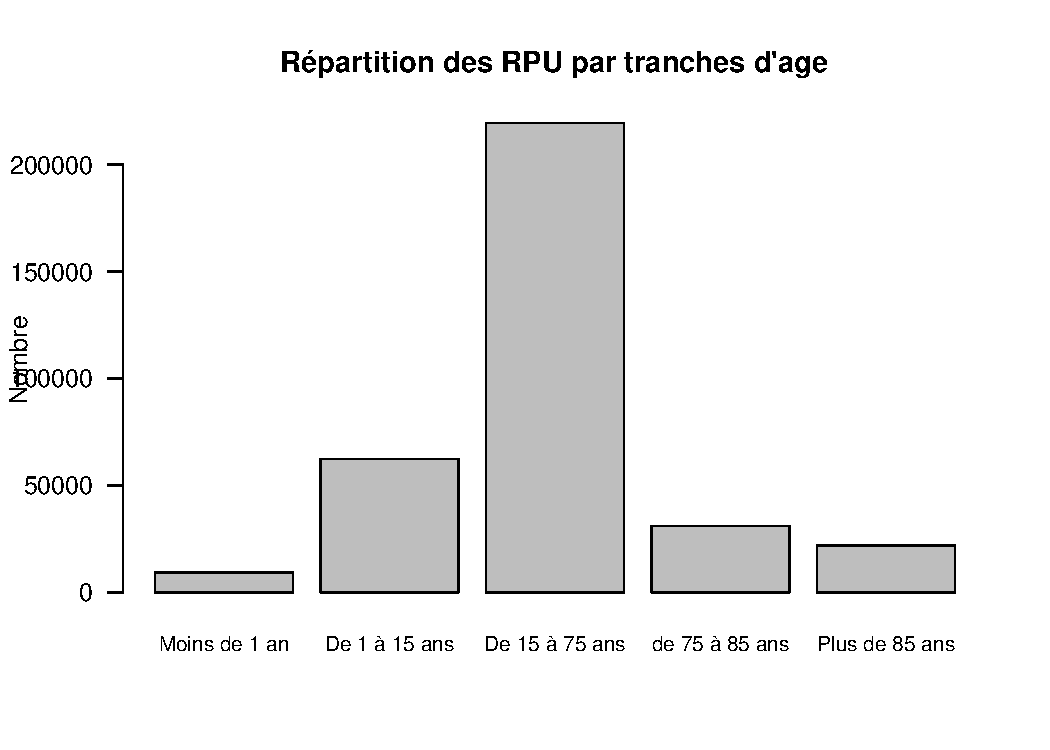
\includegraphics[width=\maxwidth]{figure/tranches_age1-1} 

\end{knitrout}
\captionof{figure}{Répartition des RPU par tanches d'âge}
\label{fig:tranches_age1}
\end{center}

%\end{figure}

% ### Age 2
%----------

% latex table generated in R 3.1.2 by xtable 1.7-1 package
% Sat Nov  8 20:45:05 2014
\begin{table}[ht]
\centering
\begin{tabular}{rrrr}
  \hline
 & Pédiatrie & Adulte $<$ 75 ans & Gériatrie \\ 
  \hline
n & 83 445,00 & 207 547,00 & 53 038,00 \\ 
  \% & 24,26 & 60,33 & 15,42 \\ 
   \hline
\end{tabular}
\caption{Répartition en trois classe d'âge telles qu'elles sont définies par le serveur régional de veille et d'alerte} 
\label{tranche_age2}
\end{table}


\begin{itemize}
  \item Pédiatrie:  24 \%
  \item Gériatrie:  15 \%
\end{itemize}

Voir figure \ref{fig:tranches_age2} page \pageref{fig:tranches_age2} et table \ref{tranche_age2} page \pageref{tranche_age2}

%\begin{figure}
\begin{center}
\begin{knitrout}
\definecolor{shadecolor}{rgb}{0.969, 0.969, 0.969}\color{fgcolor}
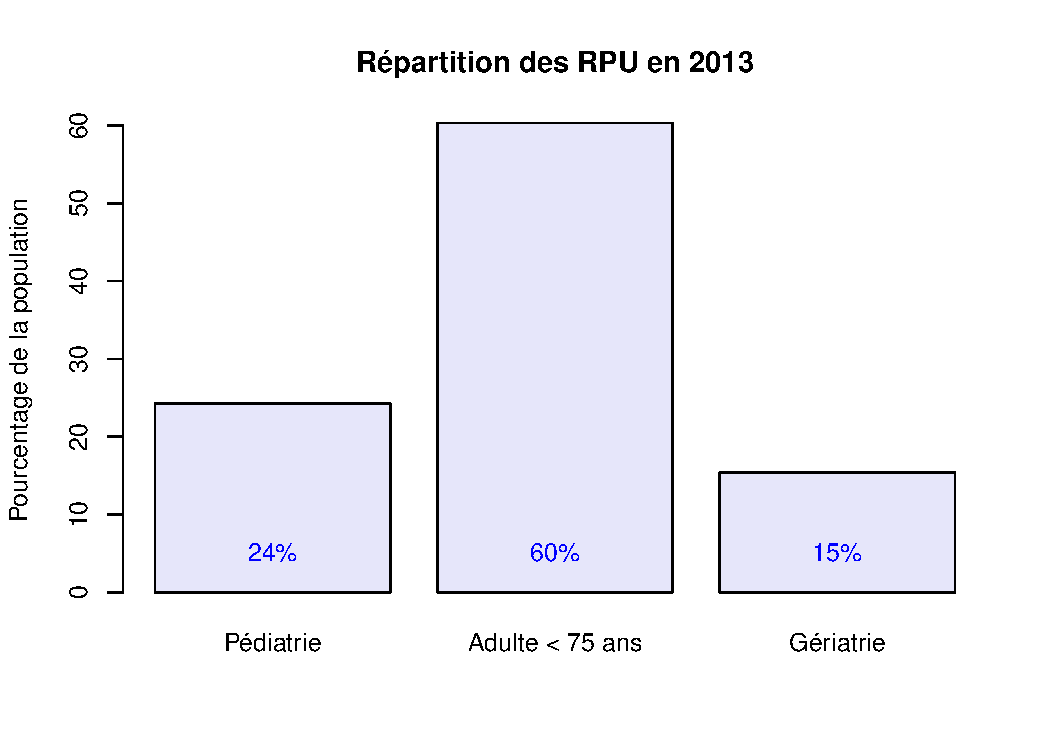
\includegraphics[width=\maxwidth]{figure/tranches_age21-1} 

\end{knitrout}
\captionof{figure}{Répartition des RPU en trois classes d'âge.}
\label{fig:tranches_age2}
\end{center}

%\end{figure}

% ### Age3
%---------



% # Affichage
%\begin{figure}
\begin{center}
\begin{knitrout}
\definecolor{shadecolor}{rgb}{0.969, 0.969, 0.969}\color{fgcolor}
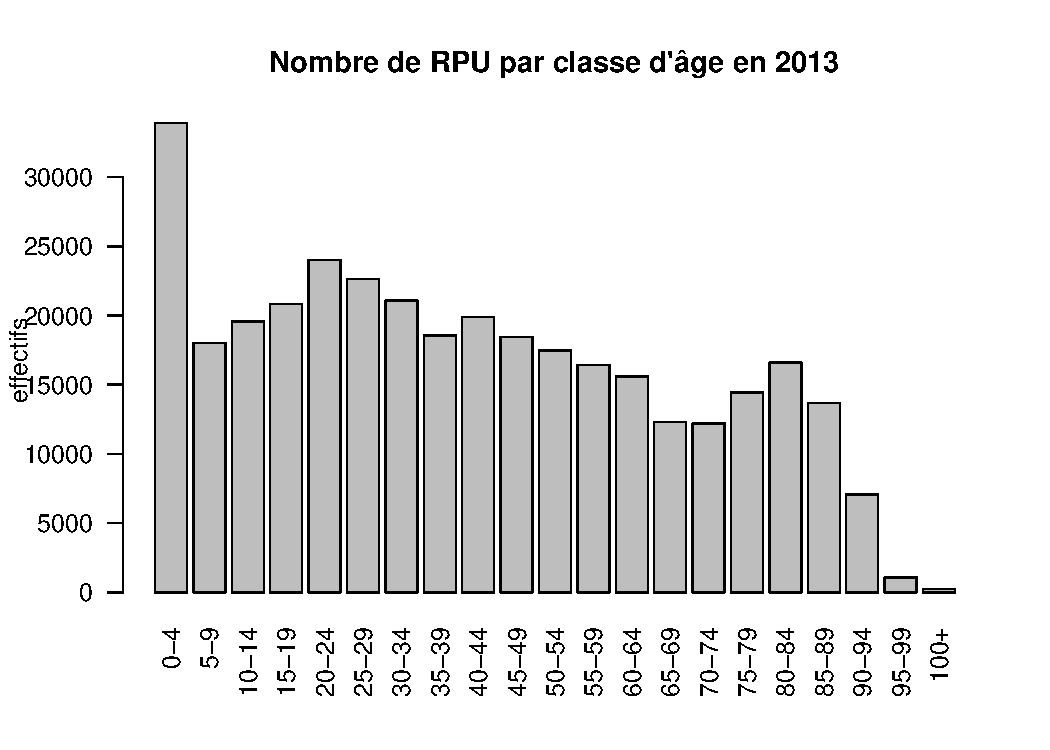
\includegraphics[width=\maxwidth]{figure/affiche_age3-1} 

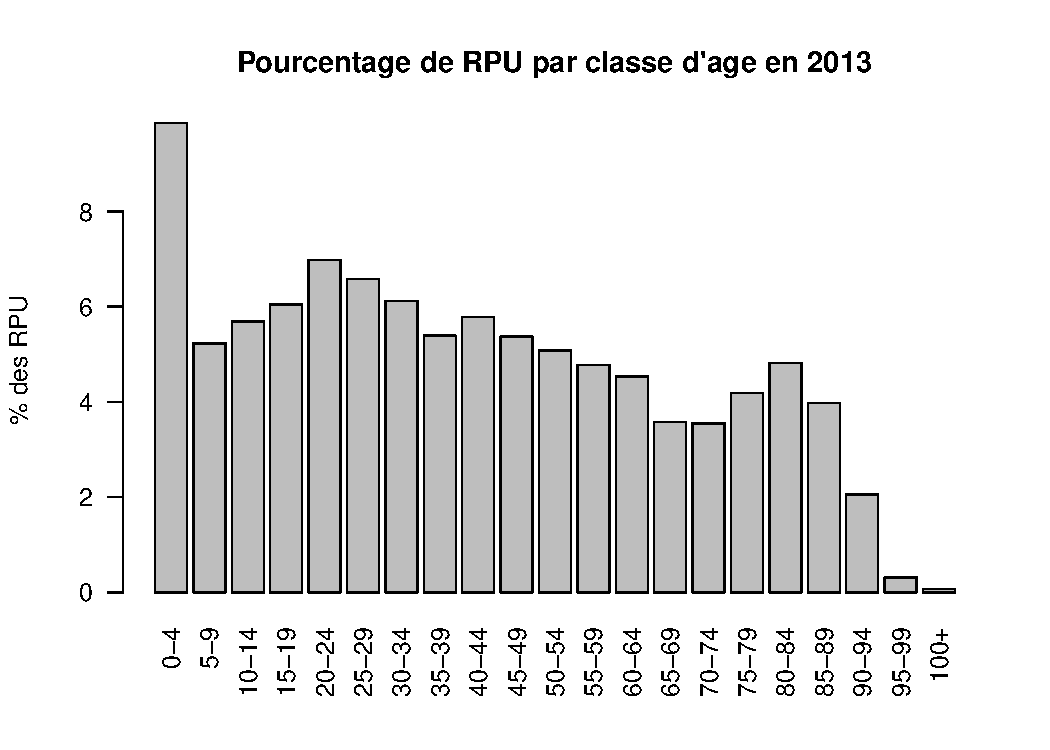
\includegraphics[width=\maxwidth]{figure/affiche_age3-2} 

\end{knitrout}
\end{center}
\captionof{figure}{Répartition des RPU par tanches d'âge}
\label{fig:tranches_age3}
%\end{figure}


\subsection*{Pyramide des âges des consultants}
%--------------------------------------------------------
\index{âge!et sexe}

% latex table generated in R 3.1.2 by xtable 1.7-1 package
% Sat Nov  8 20:45:05 2014
\begin{table}[ht]
\centering
\begin{tabular}{rrr}
  \hline
 & H & F \\ 
  \hline
0-4 & 19 105 & 14 812 \\ 
  5-9 & 10 077 & 7 930 \\ 
  10-14 & 10 666 & 8 915 \\ 
  15-19 & 10 959 & 9 868 \\ 
  20-24 & 12 667 & 11 359 \\ 
  25-29 & 12 383 & 10 263 \\ 
  30-34 & 11 813 & 9 259 \\ 
  35-39 & 10 443 & 8 109 \\ 
  40-44 & 11 170 & 8 731 \\ 
  45-49 & 10 172 & 8 291 \\ 
  50-54 & 9 371 & 8 093 \\ 
  55-59 & 8 772 & 7 669 \\ 
  60-64 & 8 609 & 6 973 \\ 
  65-69 & 6 811 & 5 498 \\ 
  70-74 & 6 438 & 5 762 \\ 
  75-79 & 6 937 & 7 489 \\ 
  80-84 & 7 034 & 9 561 \\ 
  85-89 & 4 562 & 9 127 \\ 
  90-94 & 1 942 & 5 118 \\ 
  95-99 & 235 & 833 \\ 
  100+ &  83 & 149 \\ 
   \hline
\end{tabular}
\caption[Répartition par âges et sexe]{Distribution des RPU par âges et sexe. Le découpage des âges en tranche de 5 ans correspond au découpage de l'INSEE} 
\label{tab:age_sexe}
\end{table}


% pyramide des ages

%\begin{figure}
\begin{center}
\begin{knitrout}
\definecolor{shadecolor}{rgb}{0.969, 0.969, 0.969}\color{fgcolor}
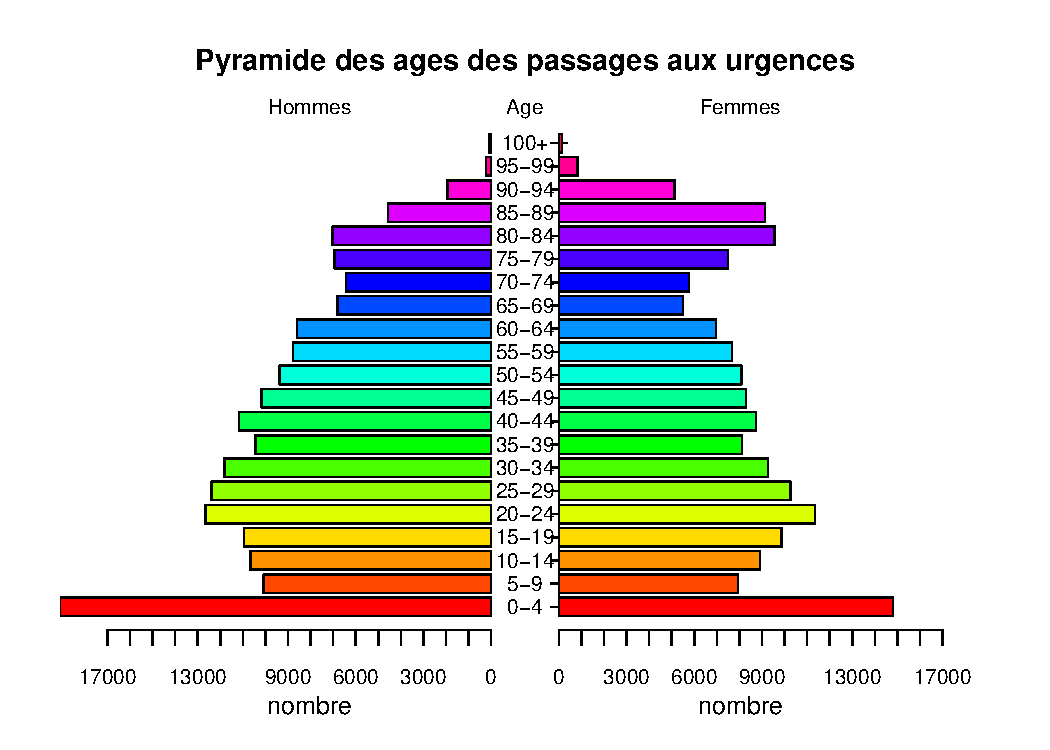
\includegraphics[width=\maxwidth]{figure/pyr_consult-1} 

\end{knitrout}
\end{center}
\captionof{figure}{Pyramide des âges des consultants}
\label{fig:pyr_consult}
%\end{figure}

% en pourcentages

% latex table generated in R 3.1.2 by xtable 1.7-1 package
% Sat Nov  8 20:45:05 2014
\begin{table}[ht]
\centering
\begin{tabular}{rrr}
  \hline
 & H & F \\ 
  \hline
0-4 & 5,55 & 4,31 \\ 
  5-9 & 2,93 & 2,30 \\ 
  10-14 & 3,10 & 2,59 \\ 
  15-19 & 3,19 & 2,87 \\ 
  20-24 & 3,68 & 3,30 \\ 
  25-29 & 3,60 & 2,98 \\ 
  30-34 & 3,43 & 2,69 \\ 
  35-39 & 3,04 & 2,36 \\ 
  40-44 & 3,25 & 2,54 \\ 
  45-49 & 2,96 & 2,41 \\ 
  50-54 & 2,72 & 2,35 \\ 
  55-59 & 2,55 & 2,23 \\ 
  60-64 & 2,50 & 2,03 \\ 
  65-69 & 1,98 & 1,60 \\ 
  70-74 & 1,87 & 1,67 \\ 
  75-79 & 2,02 & 2,18 \\ 
  80-84 & 2,04 & 2,78 \\ 
  85-89 & 1,33 & 2,65 \\ 
  90-94 & 0,56 & 1,49 \\ 
  95-99 & 0,07 & 0,24 \\ 
  100+ & 0,02 & 0,04 \\ 
   \hline
\end{tabular}
\caption[Sexe et age en pourcentages]{Répartition en pourcentages des classes d'âge en fonction du sexe des consultants} 
\label{tab:pyr_p100}
\end{table}



%\begin{figure}
\begin{center}
\begin{knitrout}
\definecolor{shadecolor}{rgb}{0.969, 0.969, 0.969}\color{fgcolor}
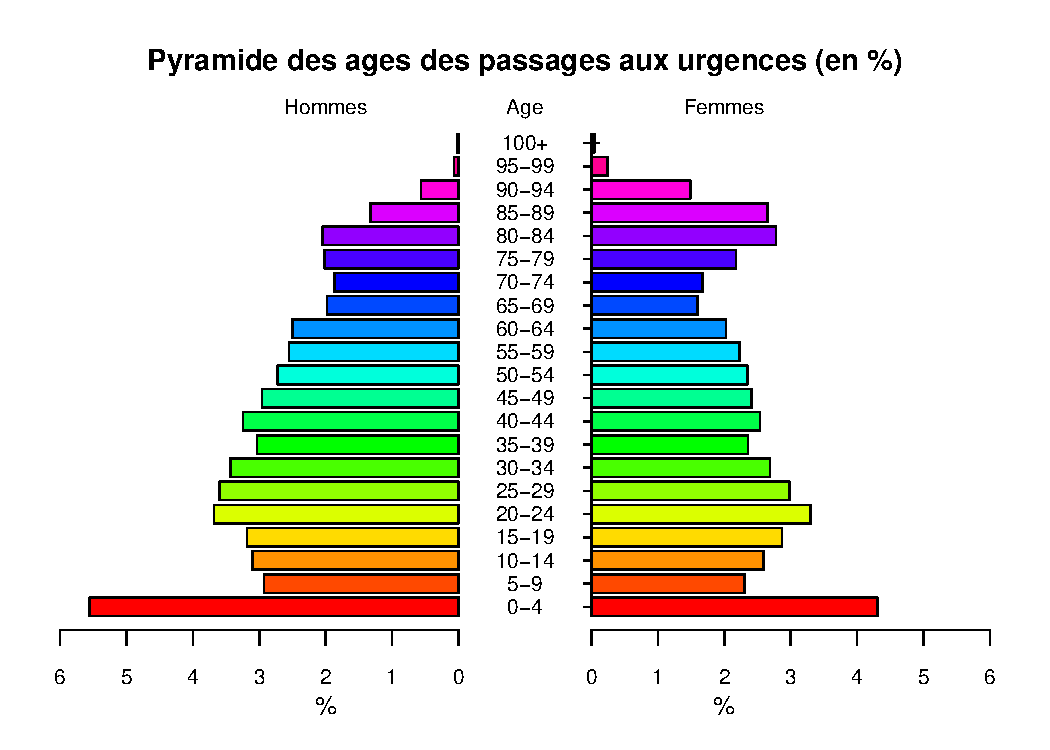
\includegraphics[width=\maxwidth]{figure/pyr_consult_p100-1} 

\end{knitrout}
\end{center}
\caption{figure}{Pyramide des âges des consultants (exprimés en pourcentages)}
\label{fig:tranches_age31}
%\end{figure}


\subsection*{Comparaison des pyramides des âges consultants-population générale}
--------------------------------------------------------------------------------

%\begin{figure}
\begin{center}
\begin{knitrout}
\definecolor{shadecolor}{rgb}{0.969, 0.969, 0.969}\color{fgcolor}
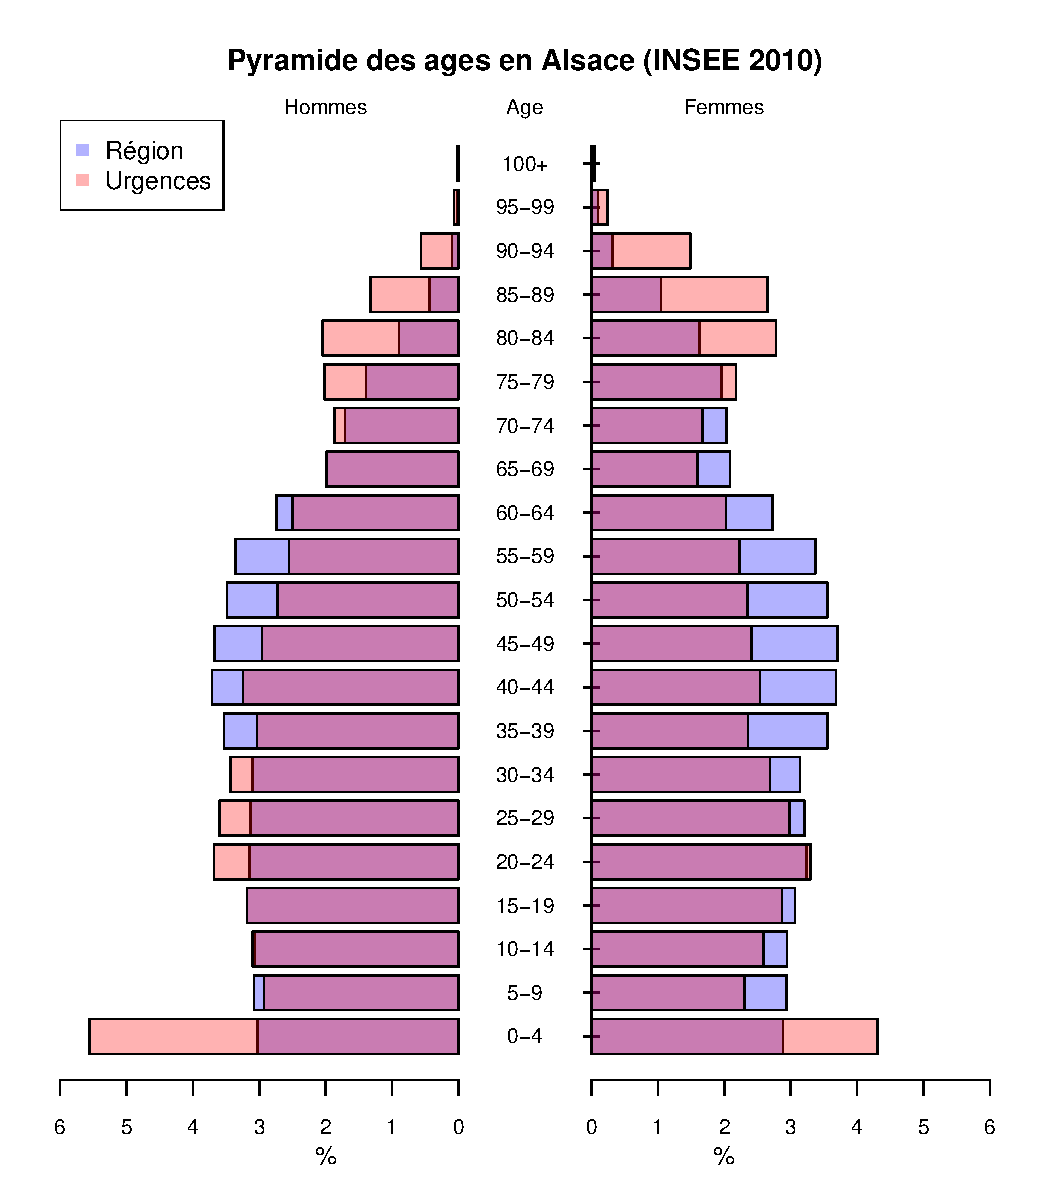
\includegraphics[width=\maxwidth]{figure/comp_pyramides-1} 

\end{knitrout}
\captionof{figure}{Pyramide des âges des consultants aux urgences comparés à la population générale. Les âges extrêmes et les adultes jeunes fréquentent davantage les SU.}
\label{fig:pyr_rpu_popgen}
\end{center}

%\end{figure}

La pyramide des âges des personnes consultant aux urgences n'est pas superposable à celle de la population générale (figure \ref{fig:pyr_rpu_popgen} page \pageref{fig:pyr_rpu_popgen}). Les enfants, les adultes jeunes et les personnes agées sont sur-représentés alors que les tranches d'âge 35-65 ans sont sous-représentées.


\subsection*{Taux de recours aux urgences par âge et par sexe}
%--------------------------------------------------------

Le taux de recours est le rapport du nombre de RPU produits dans une classe d'âge donnée, à l'effectif de cette classe dans la population alsacienne. 

%\begin{figure}
\begin{center}
\begin{knitrout}
\definecolor{shadecolor}{rgb}{0.969, 0.969, 0.969}\color{fgcolor}
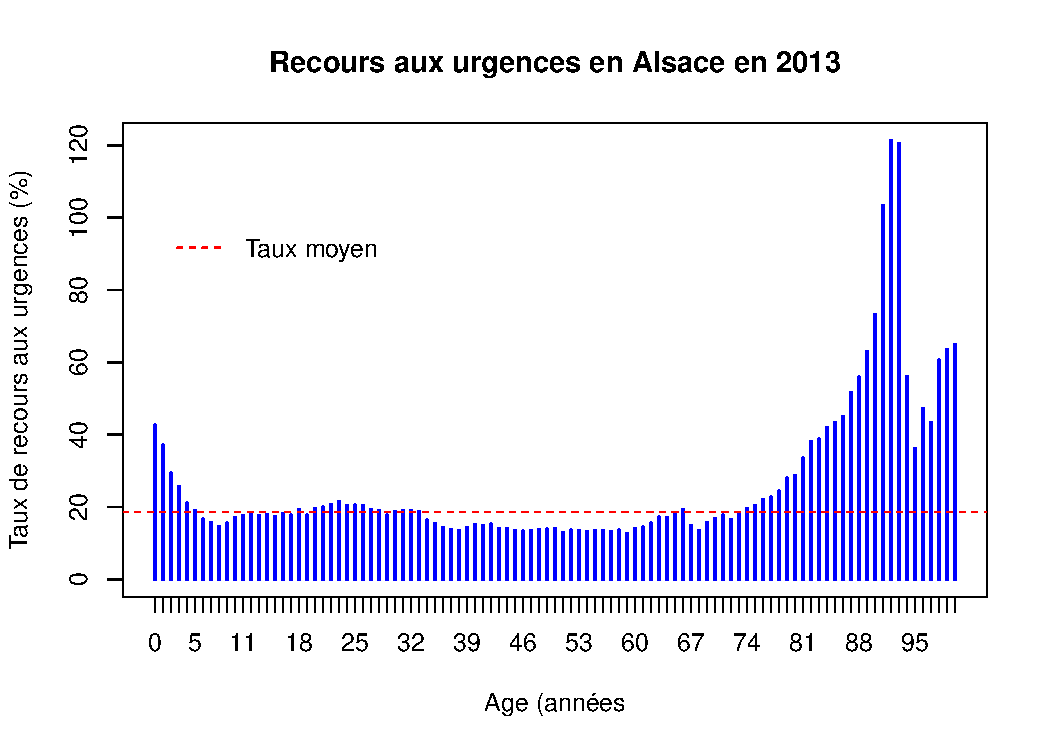
\includegraphics[width=\maxwidth]{figure/alsace_recours-1} 

\end{knitrout}
\captionof{figure}{Taux de recours aux urgences en 2013 selon la classe d'age. Le taux de recours est le rapport du nombre de RPU dans une classe d'âge donnée, à l'effectif de cette classe dans la population alsacienne.}
\label{fig:recours_su}
\end{center}

%\end{figure}

Le taux moyen de recours aux urgences en 2013 est de \textbf{19 \%}. Ce taux reste assez stable jusque vers 70 ans puis croît de façon exponentielle avec l'âge (figure \ref{fig:recours_su} page \pageref{fig:recours_su}). Pour la tranche d'âge de 90 ans, on note une sur-représentation de ces patients, le nombre de consultants dépassant la population de cette classe d'âge, traduisant un mode de recours itératif aux services d'urgence.

\subsection*{Les Centenaires}
%--------------------------------
\index{Centenaires (les)}
\label{centenaires}



Entrent dans cette catégorie les patients de 100 ans et plus. En 2013, \textbf{242 centenaires} ont été pris en charge par les services d'urgence (0.07  \% des RPU).  
Le recensement 2010 fait état de \textbf{358} centenaires en Alsace. Le taux de recours aux urgences pour cette population particulière s'élève à  68 \%.


\subsection*{Evolution du sex-ratio en fonction de l'age}
%-----------------------------------------------------------
\index{sex ratio}



% latex table generated in R 3.1.2 by xtable 1.7-1 package
% Sat Nov  8 20:45:06 2014
\begin{table}[ht]
\centering
\begin{tabular}{rrrrr}
  \hline
 & Femmes & I & Hommes & sex ratio \\ 
  \hline
0-4 & 14 812,00 & 1,00 & 19 105,00 & 1,29 \\ 
  5-9 & 7 930,00 & 1,00 & 10 077,00 & 1,27 \\ 
  10-14 & 8 915,00 & 0,00 & 10 666,00 & 1,20 \\ 
  15-19 & 9 868,00 & 2,00 & 10 959,00 & 1,11 \\ 
  20-24 & 11 359,00 & 0,00 & 12 667,00 & 1,12 \\ 
  25-29 & 10 263,00 & 0,00 & 12 383,00 & 1,21 \\ 
  30-34 & 9 259,00 & 0,00 & 11 813,00 & 1,28 \\ 
  35-39 & 8 109,00 & 0,00 & 10 443,00 & 1,29 \\ 
  40-44 & 8 731,00 & 0,00 & 11 170,00 & 1,28 \\ 
  45-49 & 8 291,00 & 0,00 & 10 172,00 & 1,23 \\ 
  50-54 & 8 093,00 & 0,00 & 9 371,00 & 1,16 \\ 
  55-59 & 7 669,00 & 0,00 & 8 772,00 & 1,14 \\ 
  60-64 & 6 973,00 & 0,00 & 8 609,00 & 1,23 \\ 
  65-69 & 5 498,00 & 0,00 & 6 811,00 & 1,24 \\ 
  70-74 & 5 762,00 & 0,00 & 6 438,00 & 1,12 \\ 
  75-79 & 7 489,00 & 0,00 & 6 937,00 & 0,93 \\ 
  80-84 & 9 561,00 & 1,00 & 7 034,00 & 0,74 \\ 
  85-89 & 9 127,00 & 0,00 & 4 562,00 & 0,50 \\ 
  90-94 & 5 118,00 & 0,00 & 1 942,00 & 0,38 \\ 
  95-99 & 833,00 & 0,00 & 235,00 & 0,28 \\ 
  100+ & 149,00 & 0,00 & 83,00 & 0,56 \\ 
   \hline
\end{tabular}
\caption[]{Répartition des consultants aux urgences par tranche de cinq ans en fonction du sexe (I = sexe indéterminé).} 
\label{tab:sr2}
\end{table}



Le rapport de masculinité ou sex ratio est de 1.1 pour l'ensemble des RPU. Ce chiffre reste stable jusque vers l'age de 77 ans puis s'inverse, reflet d'une espérance de vie plus élevée pour les femmes (figure \ref{fig:sex-ratio} page \pageref{fig:sex-ratio}).

%\begin{figure}
\begin{center}
\begin{knitrout}
\definecolor{shadecolor}{rgb}{0.969, 0.969, 0.969}\color{fgcolor}
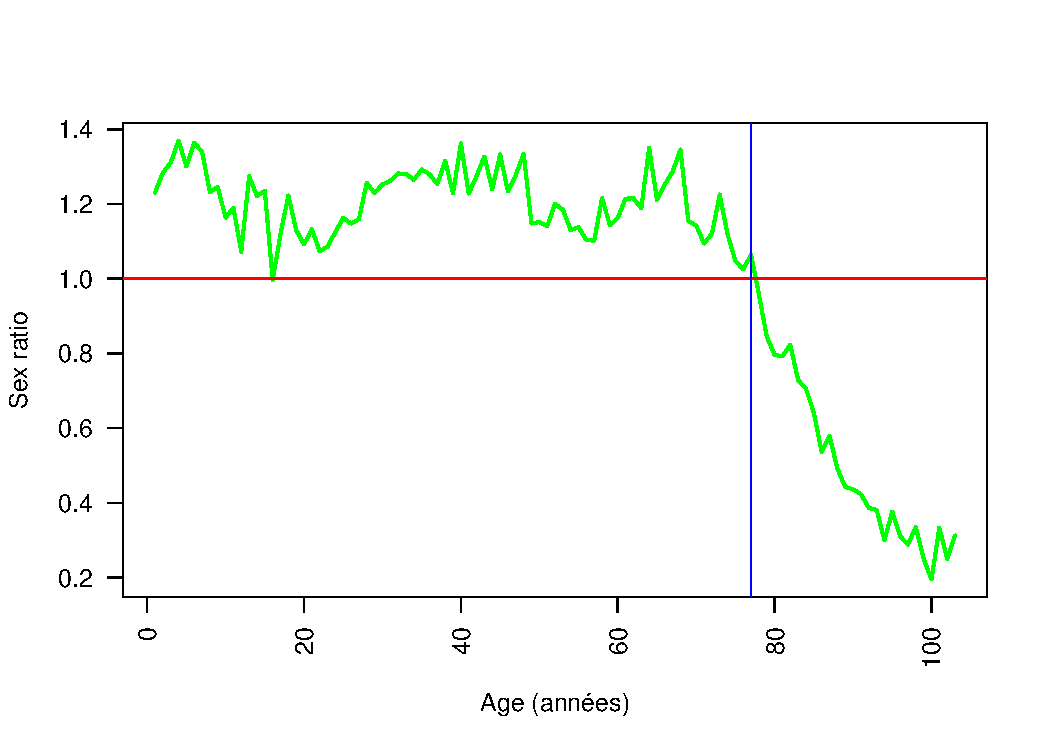
\includegraphics[width=\maxwidth]{figure/sr_graphe-1} 

\end{knitrout}
\caption{Evolution du sex ratio en fonction de l'âge)}
\label{fig:sex-ratio}
\end{center}

%\end{figure}


\newpage
\chapter{Analyse de la gravité}

% Analyse de la gravité
%gravite.Rnw

\index{Gravité (CCMU)}
\index{CCMU}

La gravité de la pathologie s'exprime au travers de la Classification Clinique des Maladies aux Urgences (CCMU). Cette classification répond à une logique médicale mais les items qui la composent lui confèrent une approche très subjective qui nuit à sa repoductibilité entre différents observateurs. C'est pourquoi une majorité d'entre eux souhaitent son abandon mais  faute d'un consenssus autour d'un autre indicateur de gravité, son usage perdure.

\section{La classification CCMU}

\begin{itemize}
  \item CCMU 1: situation stable, absence d'acte complémentaire diagnostic ou thérapeutique
  \item CCMU 2: situation stable, réalisation d'acte complémentaire, diagnostic ou thérapeutique
  \item CCMU 3: situation susceptible de s'aggraver sans mise en jeu du pronostic vital
  \item CCMU 4: pronostic vital engagé, pas de manoeuvre de réanimation immédiate
  \item CCMU 5: pronostic vital engagé, manoeuvres de réanimation immédiates
  
  \item CCMU P: problème psychiatrique ou psychologique dominant, isolé ou associé à une pathologie somatique jugée stable. Pas d'actes diagnostiques ou thérapeutiques complémentaires.
  \item CCMU D: patient arrivé décédé aux urgences. Pas de manoeuvres de réanimation.
\end{itemize}

\section{Analyse CCMU régionale}

% latex table generated in R 3.1.2 by xtable 1.7-1 package
% Sat Nov  8 20:45:06 2014
\begin{table}[ht]
\centering
\begin{tabular}{rrrrrrrr}
  \hline
 & 1 & 2 & 3 & 4 & 5 & D & P \\ 
  \hline
n & 38 839,0 & 209 300,0 & 41 078,0 & 3 561,0 & 868,0 & 38,0 & 1 380,0 \\ 
  \% & 13,2 & 70,9 & 13,9 & 1,2 & 0,3 & 0,0 & 0,5 \\ 
   \hline
\end{tabular}
\caption[Répartition des RPU selon la CCMU]{Ventilation des RPU selon la classification CCMU en 2013. Les résultats sont données en valeur absolue et en pourcentage.} 
\label{fig:ccmu}
\end{table}


\section{CCMU par département}

% latex table generated in R 3.1.2 by xtable 1.7-1 package
% Sat Nov  8 20:45:07 2014
\begin{table}[ht]
\centering
\begin{tabular}{rrrrrrrr}
  \hline
 & 1 & 2 & 3 & 4 & 5 & D & P \\ 
  \hline
67 & 9 623 & 87 166 & 18 779 & 1 676 & 393 &  25 & 225 \\ 
  68 & 29 216 & 122 134 & 22 299 & 1 885 & 475 &  13 & 1 155 \\ 
   \hline
\end{tabular}
\end{table}

	Pearson's Chi-squared test

data:  t
X-squared = 4965, df = 6, p-value < 2.2e-16



soit en pourcentages:

% latex table generated in R 3.1.2 by xtable 1.7-1 package
% Sat Nov  8 20:45:07 2014
\begin{table}[ht]
\centering
\begin{tabular}{rrrrrrrr}
  \hline
 & 1 & 2 & 3 & 4 & 5 & D & P \\ 
  \hline
67 & 3,26 & 29,54 & 6,36 & 0,57 & 0,13 & 0,01 & 0,08 \\ 
  68 & 9,90 & 41,39 & 7,56 & 0,64 & 0,16 & 0,00 & 0,39 \\ 
   \hline
\end{tabular}
\end{table}


\section{CCMU par établissement}

% latex table generated in R 3.1.2 by xtable 1.7-1 package
% Sat Nov  8 20:45:07 2014
\begin{table}[ht]
\centering
\begin{tabular}{rrrrrrrr}
  \hline
 & 1 & 2 & 3 & 4 & 5 & D & P \\ 
  \hline
3Fr & 1 431 & 13 577 & 102 & 8 & 10 & 3 & 1 \\ 
  Alk & 373 & 8 238 & 1 950 & 0 & 0 & 0 & 2 \\ 
  Col & 21 093 & 32 409 & 9 039 & 566 & 186 & 8 & 1 122 \\ 
  Dia & 50 & 22 435 & 5 742 & 15 & 2 & 1 & 0 \\ 
  Geb & 881 & 14 072 & 77 & 19 & 3 & 1 & 30 \\ 
  Hag & 2 885 & 18 727 & 4 756 & 388 & 170 & 18 & 9 \\ 
  Hus & 1 750 & 9 225 & 4 732 & 576 & 132 & 1 & 0 \\ 
  Mul & 5 388 & 31 403 & 5 389 & 1 277 & 274 & 0 & 0 \\ 
  Odi & 1 105 & 23 237 & 1 508 & 7 & 0 & 1 & 0 \\ 
  Sel & 2 717 & 19 759 & 5 648 & 492 & 58 & 3 & 172 \\ 
  Wis & 828 & 10 983 & 608 & 141 & 33 & 1 & 38 \\ 
  Sav & 338 & 5 235 & 1 527 & 72 & 0 & 1 & 6 \\ 
   \hline
\end{tabular}
\caption[CCMU et établissement]{CCMU et établissement} 
\end{table}


et en pourcentage:

% latex table generated in R 3.1.2 by xtable 1.7-1 package
% Sat Nov  8 20:45:07 2014
\begin{table}[ht]
\centering
\begin{tabular}{rrrrrrrr}
  \hline
 & 1 & 2 & 3 & 4 & 5 & D & P \\ 
  \hline
3Fr & 9,46 & 89,72 & 0,67 & 0,05 & 0,07 & 0,02 & 0,01 \\ 
  Alk & 3,53 & 77,99 & 18,46 & 0,00 & 0,00 & 0,00 & 0,02 \\ 
  Col & 32,74 & 50,31 & 14,03 & 0,88 & 0,29 & 0,01 & 1,74 \\ 
  Dia & 0,18 & 79,43 & 20,33 & 0,05 & 0,01 & 0,00 & 0,00 \\ 
  Geb & 5,84 & 93,30 & 0,51 & 0,13 & 0,02 & 0,01 & 0,20 \\ 
  Hag & 10,70 & 69,48 & 17,65 & 1,44 & 0,63 & 0,07 & 0,03 \\ 
  Hus & 10,66 & 56,20 & 28,83 & 3,51 & 0,80 & 0,01 & 0,00 \\ 
  Mul & 12,32 & 71,81 & 12,32 & 2,92 & 0,63 & 0,00 & 0,00 \\ 
  Odi & 4,27 & 89,86 & 5,83 & 0,03 & 0,00 & 0,00 & 0,00 \\ 
  Sel & 9,42 & 68,49 & 19,58 & 1,71 & 0,20 & 0,01 & 0,60 \\ 
  Wis & 6,55 & 86,95 & 4,81 & 1,12 & 0,26 & 0,01 & 0,30 \\ 
  Sav & 4,71 & 72,92 & 21,27 & 1,00 & 0,00 & 0,01 & 0,08 \\ 
   \hline
\end{tabular}
\caption[CCMU et établissement ]{CCMU et établissement (en pourcentages)} 
\label{tab:ccmu_finess_p}
\end{table}


On note des disparités importantes entre établissements (voir le tableau \ref{tab:ccmu_finess_p} page \pageref{tab:ccmu_finess_p}).

\section{CCMU et mode de sortie}

voir le tableau \ref{tab:ccmu_mode_sortie} page \pageref{tab:ccmu_mode_sortie}

% latex table generated in R 3.1.2 by xtable 1.7-1 package
% Sat Nov  8 20:45:07 2014
\begin{table}[ht]
\centering
\begin{tabular}{rrrrr}
  \hline
 & Mutation & Transfert & Domicile & Décès \\ 
  \hline
1 & 2 305 & 142 & 34 401 & 0 \\ 
  2 & 25 223 & 2 506 & 166 767 & 2 \\ 
  3 & 27 848 & 1 669 & 8 251 & 0 \\ 
  4 & 2 778 & 89 & 200 & 0 \\ 
  5 & 678 & 40 & 26 & 0 \\ 
  D & 10 & 0 & 4 & 0 \\ 
  P & 444 & 309 & 593 & 0 \\ 
   \hline
\end{tabular}
\caption[CCMU et mode de sortie]{CCMU et mode de sortie. Si globalement les décisions sont cohérentes par rapport à la gravité estimée, certaines sont surprenantes notamment en ce qui concerne les décès ou les CCMU 4 et 5 qui rentrent à domicile.} 
\label{tab:ccmu_mode_sortie}
\end{table}


\section{CCMU et destination}

voir le tableau \ref{tab:ccmu_dest} page \pageref{tab:ccmu_dest}

% latex table generated in R 3.1.2 by xtable 1.7-1 package
% Sat Nov  8 20:45:07 2014
\begin{table}[ht]
\centering
\begin{tabular}{rrrrrrr}
  \hline
 & MCO & SSR & SLD & PSY & HAD & HMS \\ 
  \hline
1 & 2 379 & 1 & 1 & 61 & 0 & 3 \\ 
  2 & 27 301 & 68 & 10 & 271 & 4 & 15 \\ 
  3 & 29 223 & 31 & 13 & 157 & 2 & 2 \\ 
  4 & 2 826 & 2 & 2 & 12 & 0 & 0 \\ 
  5 & 701 & 0 & 0 & 9 & 0 & 0 \\ 
  D & 10 & 0 & 0 & 0 & 0 & 0 \\ 
  P & 143 & 0 & 0 & 613 & 0 & 0 \\ 
   \hline
\end{tabular}
\caption[CCMU et destination]{CCMU et destination} 
\label{tab:ccmu_dest}
\end{table}


\section{CCMU et Orientation}

voir le tableau \ref{tab:ccmu_orient} page \pageref{tab:ccmu_orient}

% latex table generated in R 3.1.2 by xtable 1.7-1 package
% Sat Nov  8 20:45:07 2014
\begin{table}[ht]
\centering
\begin{tabular}{rrrrrrrr}
  \hline
 & 1 & 2 & 3 & 4 & 5 & D & P \\ 
  \hline
CHIR & 181 & 3 331 & 3 662 & 363 & 11 & 1 & 140 \\ 
  FUGUE & 67 & 141 & 22 & 0 & 0 & 0 & 9 \\ 
  HDT & 4 & 30 & 24 & 1 & 0 & 0 & 48 \\ 
  HO & 0 & 16 & 5 & 0 & 0 & 0 & 10 \\ 
  MED & 827 & 5 966 & 9 670 & 704 & 39 & 1 & 274 \\ 
  OBST & 3 & 53 & 35 & 3 & 0 & 0 & 0 \\ 
  PSA & 1 109 & 558 & 32 & 0 & 0 & 0 & 8 \\ 
  REA & 1 & 99 & 246 & 266 & 408 & 0 & 3 \\ 
  REO & 955 & 349 & 52 & 0 & 0 & 0 & 1 \\ 
  SC & 80 & 419 & 749 & 138 & 24 & 0 & 9 \\ 
  SCAM & 77 & 324 & 81 & 3 & 0 & 0 & 2 \\ 
  SI & 19 & 319 & 757 & 255 & 29 & 0 & 2 \\ 
  UHCD & 1 258 & 12 752 & 9 190 & 1 157 & 191 & 7 & 48 \\ 
   \hline
\end{tabular}
\caption[CCMU et orientation]{CCMU et orientation} 
\label{tab:ccmu_orient}
\end{table}


\newpage
\chapter{Motif de consultation}

% motif.Rnw

\index{motif de consultation}

Le motif de consultation est l'un des items les plus mal renseigné. Cela est dû en partie à l'absence de règles formelles concernant la saisie de cet élément. Une recommandation du ministère de la santé (juin 2013 \cite{12,13}) demande que le thésaurus 2013 de la SFMU \cite{9} soit utilisé.

Le thésaurus est présenté sous la forme d'un fichier Excel. L'onglet \emph{recours} liste environ \emph{150} motifs de recours aux urgences avec leur correspondance CIM10, répartis en 17 groupes. Aucune méthode n'est parfaite mais cette page constitue une base acceptable d'harmonisation des données.


% latex table generated in R 3.1.2 by xtable 1.7-1 package
% Sat Nov  8 20:45:07 2014
\begin{table}[ht]
\centering
\begin{tabular}{rlr}
  \hline
 & Etablissement & Motif (p.cent) \\ 
  \hline
1 & 3Fr & 7,22 \\ 
  2 & Alk & 23,50 \\ 
  3 & Col & 100,00 \\ 
  4 & Dia & 95,50 \\ 
  5 & Geb & 0,03 \\ 
  6 & Hag & 13,10 \\ 
  7 & Hus & 0,00 \\ 
  8 & Mul & 83,00 \\ 
  9 & Odi & 94,92 \\ 
  10 & Sel & 98,20 \\ 
  11 & Wis & 99,69 \\ 
  12 & Sav & 42,02 \\ 
   \hline
\end{tabular}
\caption[Motif de consultation]{Taux de réponse à l'item motif de consultation selon le services d'urgence} 
\label{lab:motif}
\end{table}

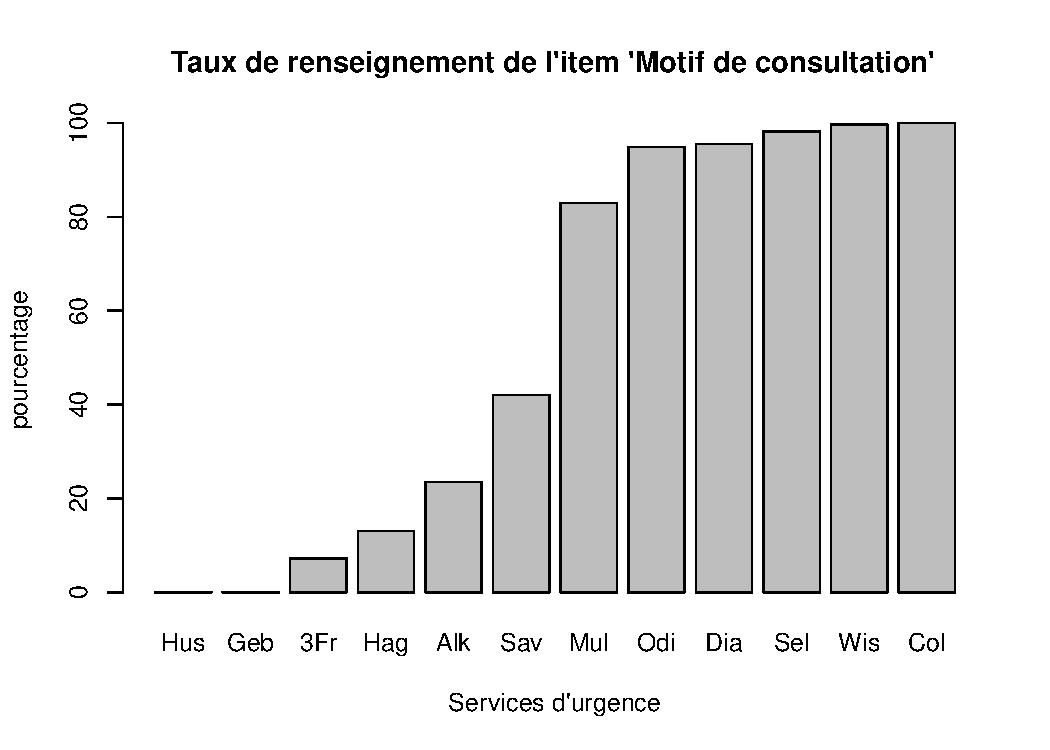
\includegraphics[width=\maxwidth]{figure/motifss-1} 


\index{exhaustivité@motif}
Le motif de consultation n'est pas renseigné dans 55 \% des cas (table \ref{lab:motif}).

Seuls six établissements ont un taux d'exhaustivité supérieur à 80\% pour cette rubrique.

Cependant seuls quelques établissements saisissent cette information sous forme normalisée qui permet de l'exploiter. Dans les autres cas il s'agit de codes propres à l'établissement ou de texte libre inexploitable.

Données non renseignées:
\begin{itemize}
  \item Guebwiller
  \item HUS
  \item Ste Anne
  \item Thann
\end{itemize}

Données renseignées mais inexploitables:
\begin{itemize}
  \item Colmar
  \item Sélestat
  \item Haguenau
\end{itemize}

Données renseignées, exploitables mais à mettre en conformité avec le thésaurus:
\begin{itemize}
  \item Mulhouse
  \item Wissembourg
  \item Altkirch (exhaustivité)
  \item Saverne
  \item Ste Odile
  \item Diaconat Fonderie
  \item Trois Frontières
\end{itemize}

\newpage
\chapter{Modalité d'admission}

% modalites.Rnw
% modalités d'admission MODE_ENTREE

\index{Mode d'entrée}

\section*{Origine des patients}

% REMARQUE dans environ 300 dossiers du mois de juin, l'item transfert est écrit "transfe  rt" ce qui nécessite un recodage.

L'immense majorité des patients provient du domicile ou son équivalent. Une très faible part des passages aux urgences sont le fait de transferts d'autres établissements ou de mutations en provenance d'autres services du même établissement.


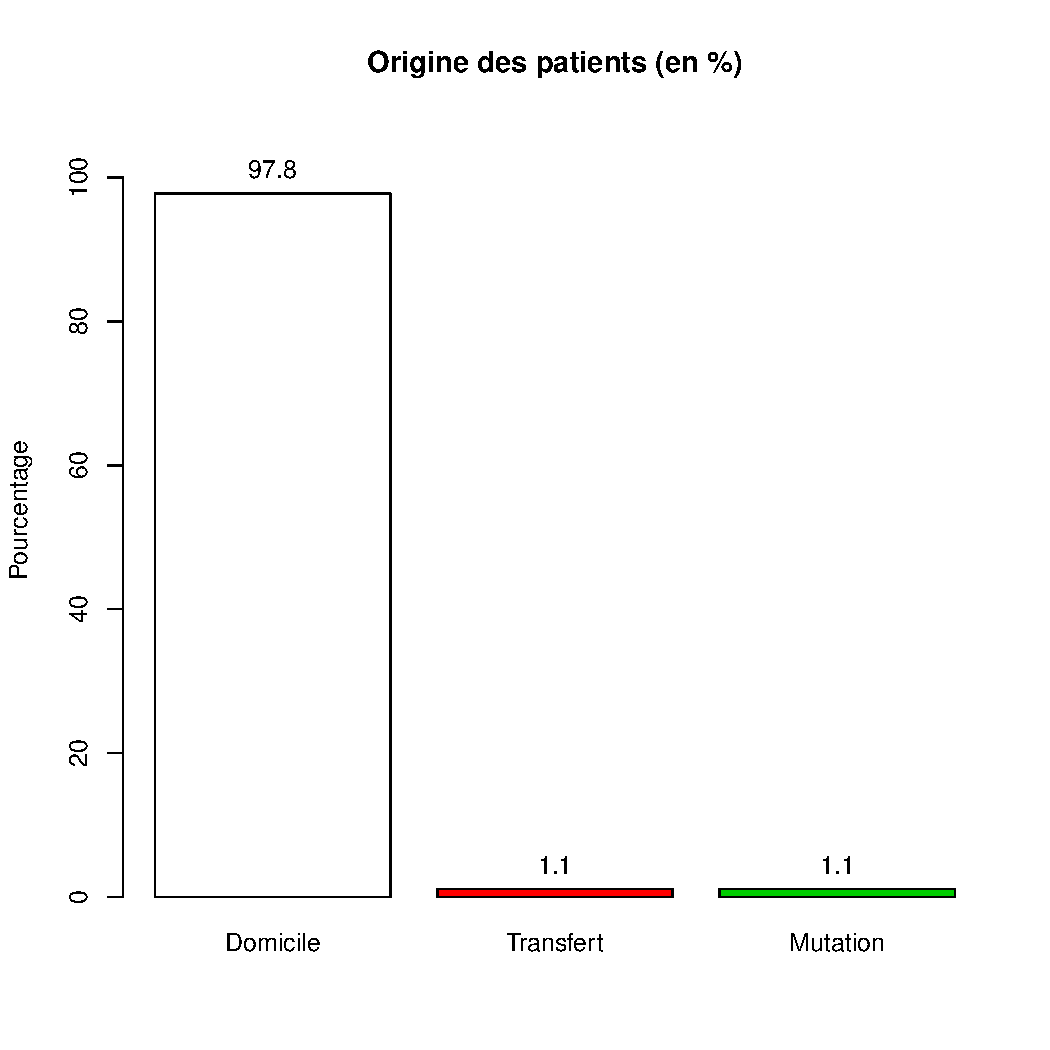
\includegraphics[width=\maxwidth]{figure/mode_entree-1} 
% latex table generated in R 3.1.2 by xtable 1.7-1 package
% Sat Nov  8 20:45:07 2014
\begin{table}[ht]
\centering
\begin{tabular}{rrrr}
  \hline
 & Fréquence & Pourcentage & Pourcentage cumulé \\ 
  \hline
Domicile & 304 289,00 & 88,40 & 97,80 \\ 
  NA's & 32 914,00 & 9,60 & 0,00 \\ 
  Mutation & 3 513,00 & 1,00 & 1,10 \\ 
  Transfert & 3 357,00 & 1,00 & 1,10 \\ 
    Total & 344 073,00 & 100,00 & 100,00 \\ 
   \hline
\end{tabular}
\caption[Origine des patients]{Origine des patients. Les deux colonnes de droite mesurent l'origine (en pourcentage) selon que l'on prenne en compte ou non les valeurs manquantes. } 
\label{origine}
\end{table}


Dans 9.6 \% des cas, l'origine du patient n'est pas précisée.

\section*{Mode de transport}
\index{Mode de transport}

La grande majorité des patients arrivent aux urgences par leurs propres moyens (PERSO). Lorsqu'ils font appel à un tiers, il s'agit le plus souvent d'une ambulance privée (AMBU), puis du SDIS (VSAB). Les transports par un vecteur médicalisé (SMUR) ou héliporté (HELI) sont rares. Enfin l'utilisation des forces de l'ordre (FO) comme moyen de transport reste marginale.


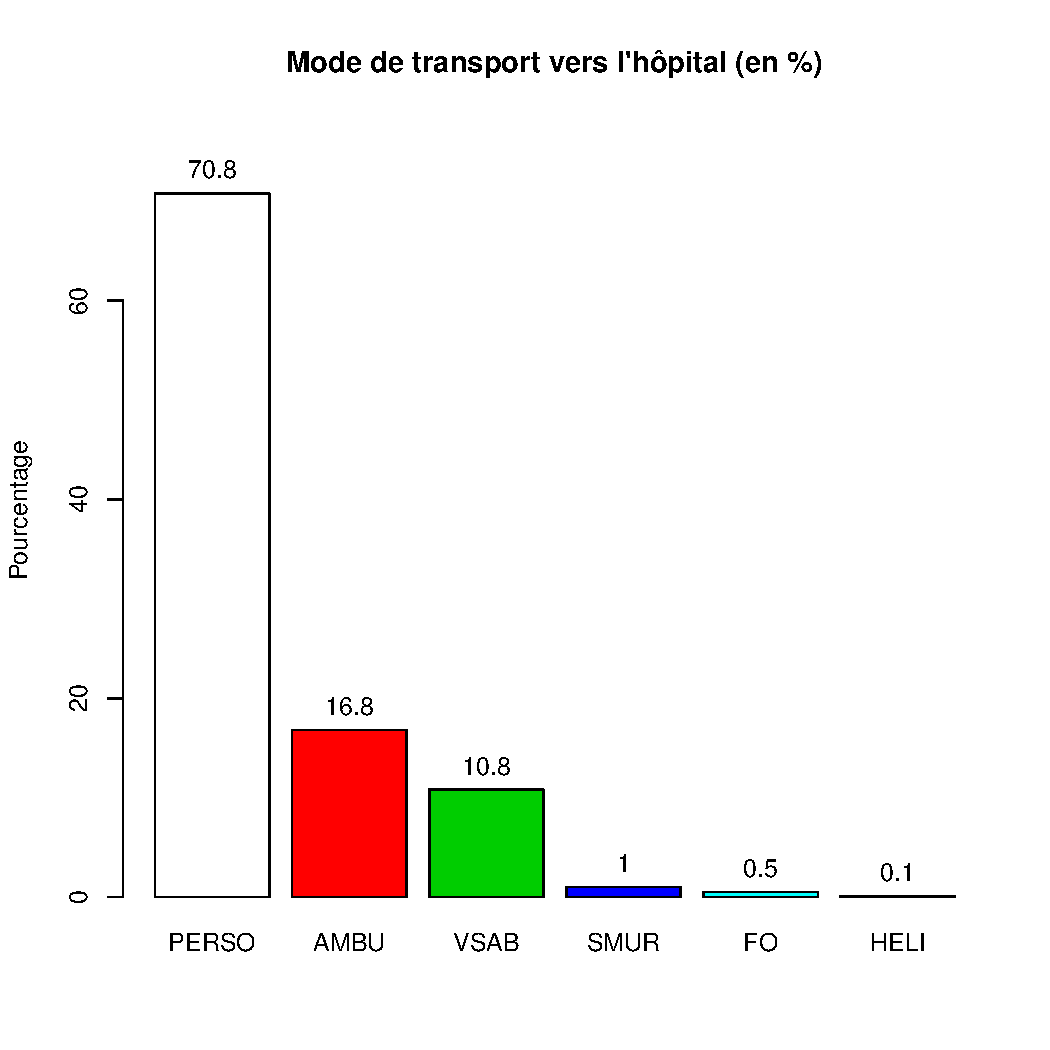
\includegraphics[width=\maxwidth]{figure/transport-1} 
% latex table generated in R 3.1.2 by xtable 1.7-1 package
% Sat Nov  8 20:45:07 2014
\begin{table}[ht]
\centering
\begin{tabular}{rrrr}
  \hline
 & Fréquence & Pourcentage & Pourcentage cumulé \\ 
  \hline
PERSO & 187 309,00 & 54,40 & 70,80 \\ 
  NA's & 79 338,00 & 23,10 & 0,00 \\ 
  AMBU & 44 602,00 & 13,00 & 16,80 \\ 
  VSAB & 28 552,00 & 8,30 & 10,80 \\ 
  SMUR & 2 609,00 & 0,80 & 1,00 \\ 
  FO & 1 456,00 & 0,40 & 0,50 \\ 
  HELI & 207,00 & 0,10 & 0,10 \\ 
    Total & 344 073,00 & 100,00 & 100,00 \\ 
   \hline
\end{tabular}
\caption[Moyens de transport]{Moyens de transport utilisés pour se rendre à l'hôpital. Les deux colonnes de droite mesurent la fréquence du moyen utilisé (en pourcentage) selon que l'on prenne en compte ou non les valeurs manquantes. } 
\label{transport}
\end{table}


Dans 0.1 \% des cas, le moyen de transport utilisé par le patient pour rejoindre l'hôpital n'est pas précisé.

%==============================
\section*{Origine géographique}
%===============================

\index{Origine géographique}

\begin{knitrout}
\definecolor{shadecolor}{rgb}{0.969, 0.969, 0.969}\color{fgcolor}
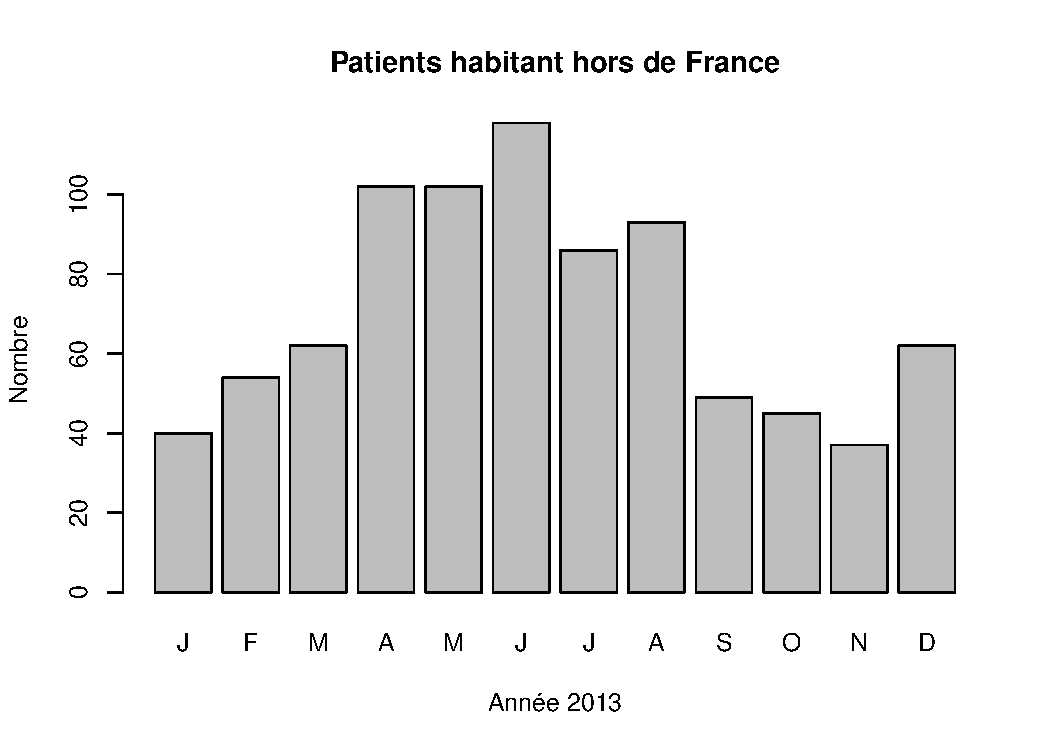
\includegraphics[width=\maxwidth]{figure/origine_geo-1} 

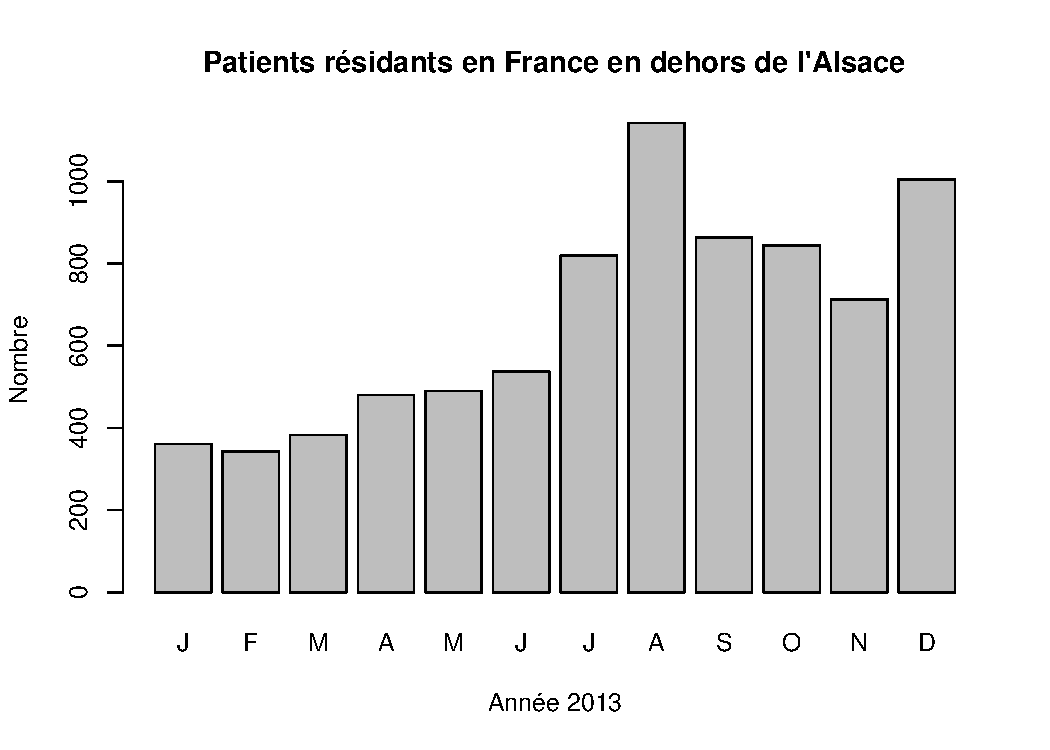
\includegraphics[width=\maxwidth]{figure/origine_geo-2} 

\end{knitrout}
Les patients consultant aux urgences sont majoritairement issus de la région Alsace. Mais l'origine est très diverse, aussi bien en provenance des autres départements français qu'hors de France:
 \begin{itemize}
   \item Alsace: 331 160 (96 \%) 
   \item hors Alsace: 7 981 (2.3 \%) 
   \item dont hors de France: 850 (0.25 \%) 
 \end{itemize}

\newpage
\chapter{Durée de passage}

% duree_passage.Rnw
\index{Durée de passage}

La durée de passage est le temps compris entre la date d'entrée et celle de sortie. Il s'agit d'une durée de transit total. Les données transmises par les RPU ne permettent pas de calculer les temps d'attente.

% ************************
% *                      *  
% *    Cas général       * 
% *                      *
% ************************

\section{Cas général}

% latex table generated in R 3.1.2 by xtable 1.7-1 package
% Sat Nov  8 20:45:09 2014
\begin{table}[ht]
\centering
\begin{tabular}{rrrrrrrrrrr}
  \hline
 & n & Min & Q25 & Moyenne & E-type & Médiane & Q75 & Max & Na & \%Na \\ 
  \hline
 & 344 073,00 & 0,00 & 55,00 & 162,70 & 194,40 & 110,00 & 204,00 & 9 867,00 & 30 344,00 & 8,80 \\ 
   \hline
\end{tabular}
\caption[temps de passage brut]{Temps de passage brut en 2013. Les valeurs non disponibles (Na) correspondent aux valeurs manquantes ou aberrantes (négatives).} 
\label{lab:temps_brut}
\end{table}


La dispersion des durées de passage est très importante, variant de -247 à \np{9 870} minutes. Les valeurs négatives sont considérées comme des valeurs manquantes. 
Finalement 30 344 durées ne sont pas renseignées (exhaustivité de 91 \% des RPU). 
La durée de passage moyenne est de 163 minutes (ecart-type 194 minutes)
Une transformation logarithmique des données permet de mieux représenter l'histogramme des durées de passage. 

%\begin{figure}[ht!]
\begin{center}
\begin{knitrout}
\definecolor{shadecolor}{rgb}{0.969, 0.969, 0.969}\color{fgcolor}
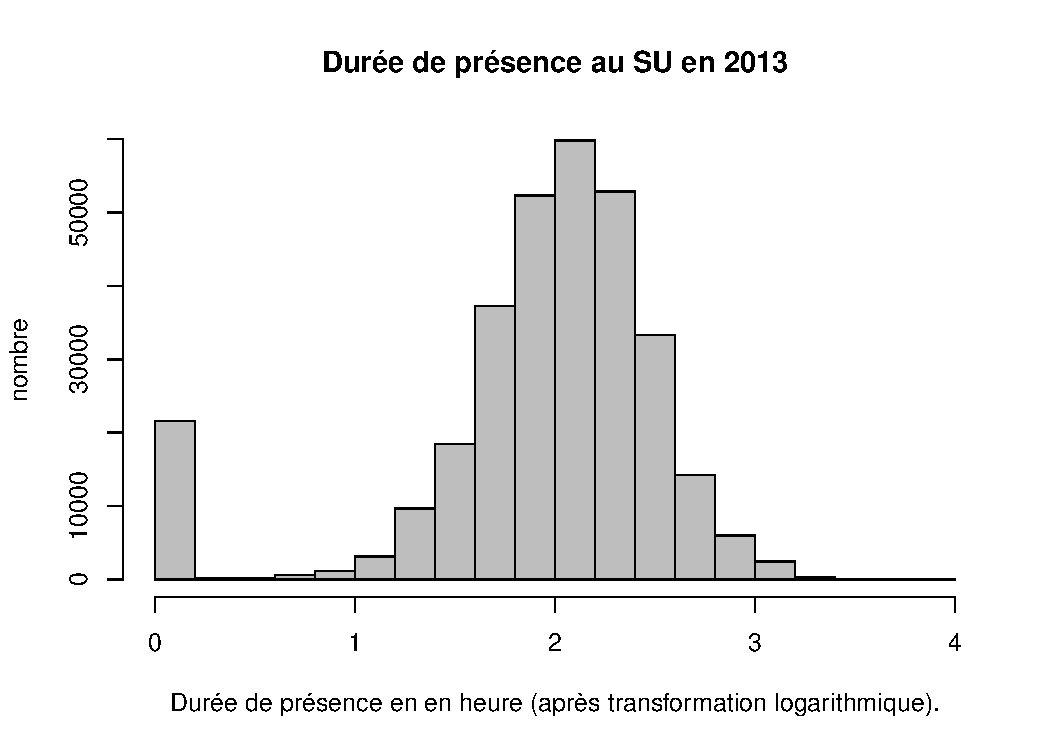
\includegraphics[width=\maxwidth]{figure/log_passages-1} 

\end{knitrout}
 \captionof{figure}{Durée de passage (log 10)}
\end{center}
%\end{figure}

la transformation log produit une courbe normale où la majorité des consultants ont une durée de présence comprise entre 10 et 1000 minutes (environ 17 heures). On nettoie les données en supprimant les enregistrements où le durée de présence est indéterminée, puis on forme 3 sous-groupes:
\begin{itemize}
  \item a moins de 10 minutes
  \item b de 10 à 1440 minutes (24 heures)
  \item c plus de 1440 minutes
\end{itemize}

% latex table generated in R 3.1.2 by xtable 1.7-1 package
% Sat Nov  8 20:45:09 2014
\begin{table}[ht]
\centering
\begin{tabular}{rrrrrrr}
  \hline
 & n & Min & Moyenne & E-type & Médiane & Q75 \\ 
  \hline
 & 289 460,00 & 10,00 & 171,50 & 173,00 & 120,00 & 214,00 \\ 
   \hline
\end{tabular}
\caption[temps de passage corrigé]{Temps de passage corrigé en 2013. Ne sont pris en compte que les temps de passage supérieurs à 10 minutes et inférieur à 24 heures.} 
\label{lab:temps_corrige}
\end{table}


Les durées de présences inférieures à 10 minutes proviennent à plus de 90\% des HUS (Erreur logicielle signalée au CRIH):
% latex table generated in R 3.1.2 by xtable 1.7-1 package
% Sat Nov  8 20:45:10 2014
\begin{table}[ht]
\centering
\begin{tabular}{rccc}
  \hline
 & Etablissement & Passages $<$ 10 mn & \% \\ 
  \hline
1 & 3Fr & 179 & 1 \\ 
  2 & Alk & 178 & 1 \\ 
  3 & Col & 283 & 1 \\ 
  4 & Dia & 246 & 1 \\ 
  5 & Geb & 108 & 0 \\ 
  6 & Hag & 165 & 1 \\ 
  7 & Hus & 21 430 & 91 \\ 
  8 & Mul & 442 & 2 \\ 
  9 & Odi & 108 & 0 \\ 
  10 & Sel & 42 & 0 \\ 
  11 & Wis & 151 & 1 \\ 
  12 & Sav & 179 & 1 \\ 
   \hline
\end{tabular}
\caption[Nombre de passages par service d'urgence de moins de 10 mn]{Nombre de RPU où la durée de passage est inférieure à 10 minutes et par établissement. On note que plus de 90 p.cent des passages des HUS sont inférieurs à cette durée.} 
\label{fig:passages10}
\end{table}


Finalement, on conserve le groupe $b$ qui regroupe la majorité (92\%) des patients. On trouve dans ce groupe une durée de présence de 171 minutes (écart-type 173 minutes, médiane 120).

%\begin{figure}[ht!]
\begin{center}
\begin{knitrout}
\definecolor{shadecolor}{rgb}{0.969, 0.969, 0.969}\color{fgcolor}
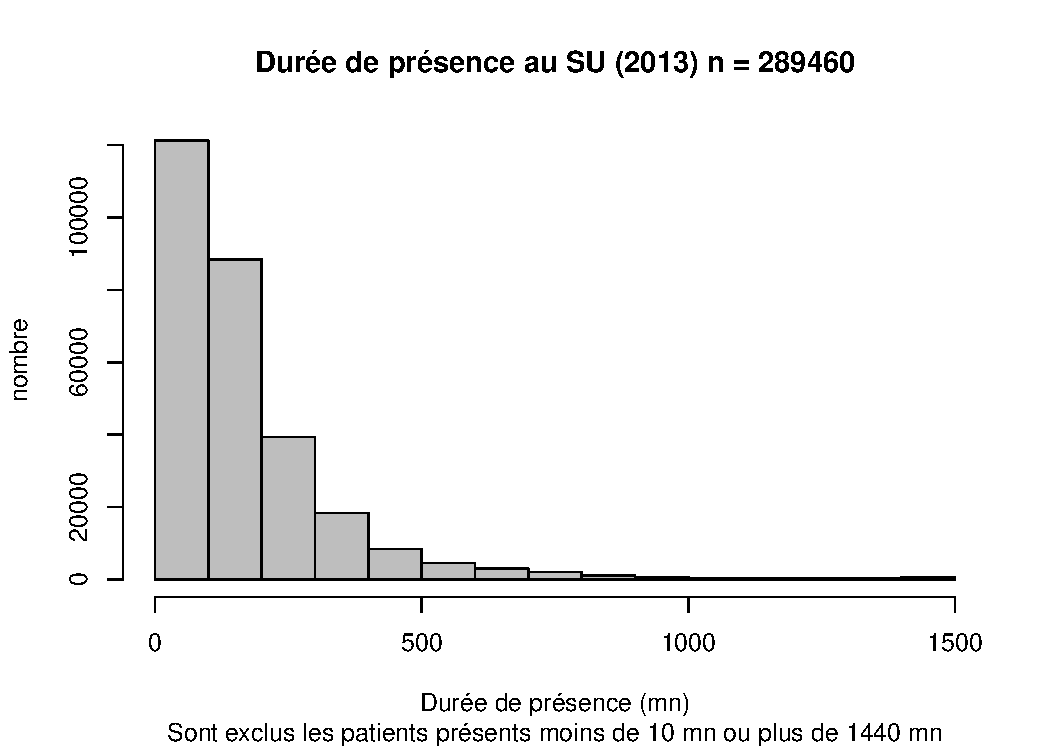
\includegraphics[width=\maxwidth]{figure/passages_clean_hist-1} 

\end{knitrout}
 \captionof{figure}{Durée de passage aux urgences}
\end{center}

% ************************
% *                      *  
% * Durée de passage     * 
% *                      *
% ************************

\section{Moyenne des durées de passages par jour}



%\begin{figure}[ht!]
\begin{center}
\begin{knitrout}
\definecolor{shadecolor}{rgb}{0.969, 0.969, 0.969}\color{fgcolor}
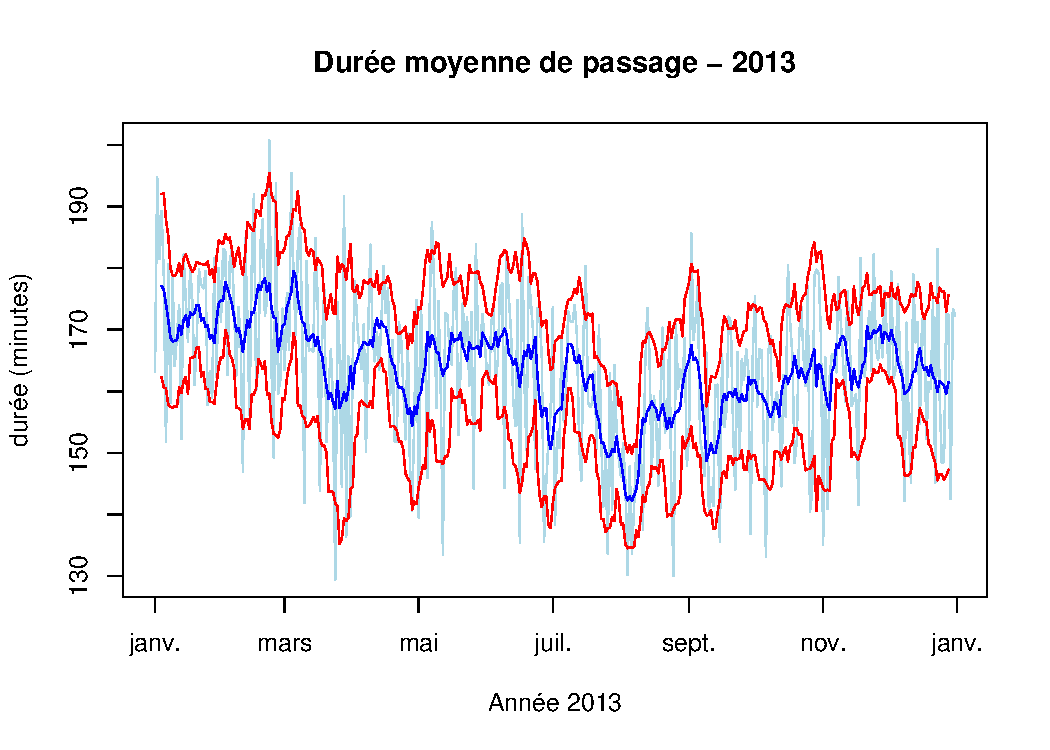
\includegraphics[width=\maxwidth]{figure/graphe_duree_moyenne_passage-1} 

\end{knitrout}
 \captionof{figure}{Durée moyenne de passage aux urgences en \ancourante)}
\end{center}



% *********************************
% *                               *
% *  Histogramme des passages     *
% *                               *
% *********************************

La distribution des durées de passage n'est pas normale mais présente une déviation axiale gauche importante (figure \ref{fig:hist_passages}). Cette notion est à prendre en considération lors de l'interprétation de la durée moyenne de passage. L'allure générale de l'histogramme évoque une loi de Poisson.

%\begin{figure}[ht!]
 \begin{center}
\begin{knitrout}
\definecolor{shadecolor}{rgb}{0.969, 0.969, 0.969}\color{fgcolor}
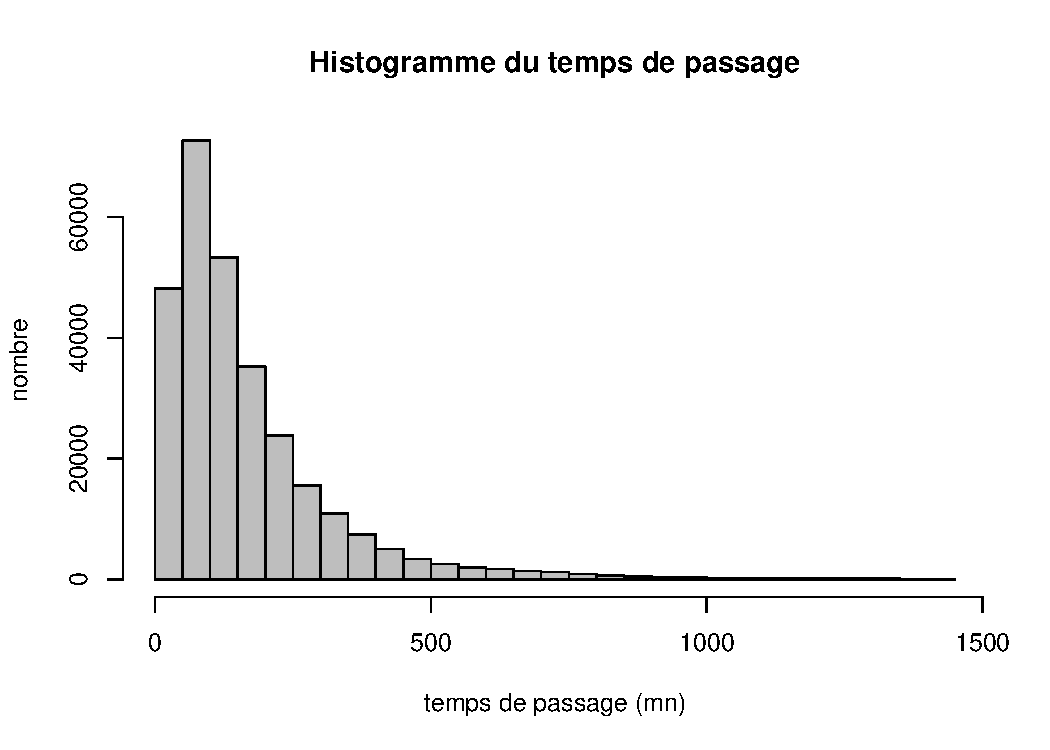
\includegraphics[width=\maxwidth]{figure/hist_tous_passages-1} 

\end{knitrout}
 \captionof{figure}{Histogramme des passages en 2013 (288 337 patients). Ne sont pris en compte que les RPU dont la durée de passage est renseignée et inférieure à 24 heures.}
 \label{fig:hist_passages}
\end{center}

% ************************
% *                      *  
% *   Selon l'heure      * 
% *                      *
% ************************

\section{Selon l'heure}

Une période de 24 heures est habituellement divisée de la manière suivante:
\begin{enumerate}
  \item \emph{journée} de 8 heures à 20 heures
  \item \emph{soirée} de 20 heures à minuit
  \item  \emph{nuit profonde} de 0 heures à 8 heures
\end{enumerate}



% latex table generated in R 3.1.2 by xtable 1.7-1 package
% Sat Nov  8 20:45:12 2014
\begin{table}[ht]
\centering
\begin{tabular}{rrrr}
  \hline
 & nuit profonde & journée & soirée \\ 
  \hline
N & 44 638,00 & 252 428,00 & 39 943,00 \\ 
  \% & 13,25 & 74,90 & 11,85 \\ 
  MJ & 122,30 & 691,58 & 109,43 \\ 
  TH & 15,29 & 57,63 & 27,36 \\ 
   \hline
\end{tabular}
\caption[Fréquentation des SU et période]{Fréquentation des urgences et période de la journée pour l'ensemble des SU d'Alsace. N: valeur absolue, MJ: moyenne journalière, TH: taux horaire. 2/3 des RRPU sont enregistrés entre 8 et 20 heures.} 
\label{tab:freq_periode}
\end{table}
% latex table generated in R 3.1.2 by xtable 1.7-1 package
% Sat Nov  8 20:45:13 2014
\begin{table}[ht]
\centering
\begin{tabular}{rrrr}
  \hline
 & nuit profonde & journée & soirée \\ 
  \hline
moyenne & 172,77 & 160,66 & 161,60 \\ 
  écart-type & 210,88 & 185,80 & 214,78 \\ 
  médiane & 107,00 & 114,00 & 95,00 \\ 
   \hline
\end{tabular}
\caption[Durée de présence et période]{Durée de présence et période de la journée. La durée de passage en nuit profonde est plus longue qu'en journée ou en soirée. Cette différence est fortement significative (p < 0.001)} 
\label{duree_periode}
\end{table}
% latex table generated in R 3.1.2 by xtable 1.7-1 package
% Sat Nov  8 20:45:13 2014
\begin{table}[ht]
\centering
\begin{tabular}{lrrrrr}
  \hline
 & DDL & Somme des carrés & Carré moyen & test F &  p \\ 
  \hline
periode & 2 & 5 394 623,01 & 2 697 311,50 & 72,78 & 0,0000 \\ 
  Residuals & 306 972 & 11 377 460 449,18 & 37 063,51 &  &  \\ 
   \hline
\end{tabular}
\caption{Comparaison des moyennes des durées de passage en fonction de la période de la journée (ANOVA). Au moins une des moyennes est significativement différente des autres.} 
\end{table}
% latex table generated in R 3.1.2 by xtable 1.7-1 package
% Sat Nov  8 20:45:13 2014
\begin{table}[ht]
\centering
\begin{tabular}{rrrrr}
  \hline
 & diff & lwr & upr & p adj \\ 
  \hline
journée-nuit profonde & -12.11 & -14.47 & -9.75 & 0.00 \\ 
  soirée-nuit profonde & -11.16 & -14.55 & -7.78 & 0.00 \\ 
  soirée-journée & 0.94 & -1.82 & 3.71 & 0.70 \\ 
   \hline
\end{tabular}
\caption{Le test HSD de Tukey montre que c'est la durée de passage en nuit profonde qui de distingue des autres. Il n'y a pas de différences entre la journée et la soirée.} 
\end{table}


%\begin{figure}[ht!]
\begin{center}
\begin{knitrout}
\definecolor{shadecolor}{rgb}{0.969, 0.969, 0.969}\color{fgcolor}
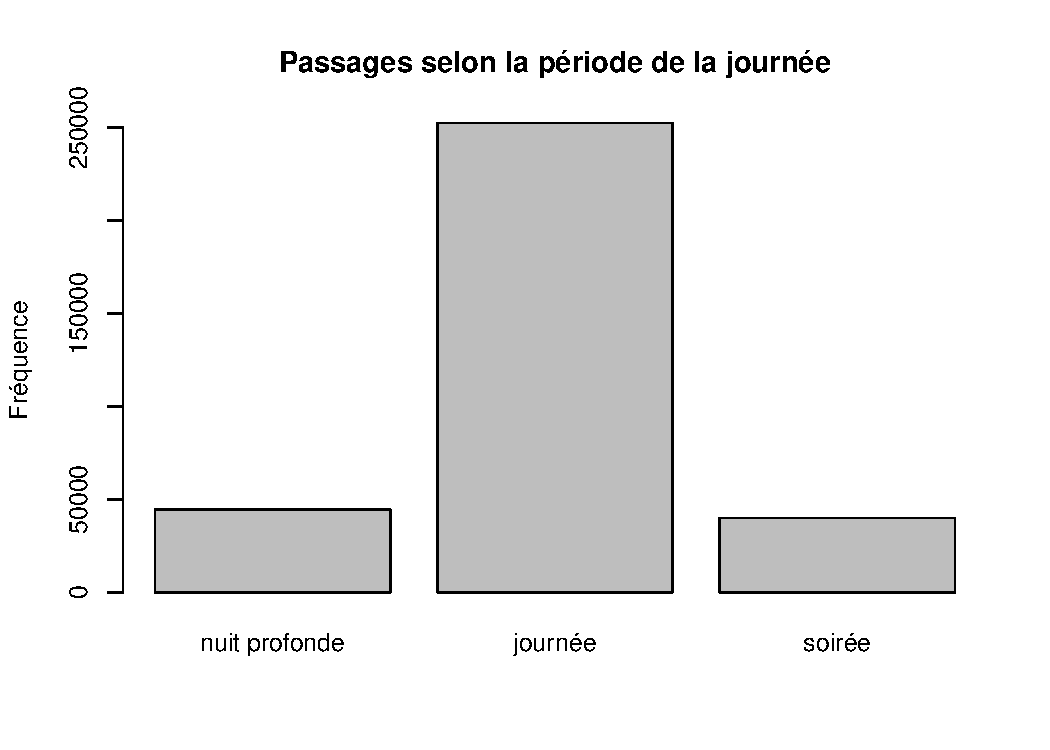
\includegraphics[width=\maxwidth]{figure/bp_periode-1} 

\end{knitrout}
 \captionof{figure}{Passages selon la période de la journée}
 \label{fig:bp_periode}
\end{center}

Les passages ont lieu majoritairement en journée (fig. \ref{fig:bp_periode} pp.\pageref{fig:bp_periode}).


%\begin{figure}[ht!]
\begin{center}
\begin{knitrout}
\definecolor{shadecolor}{rgb}{0.969, 0.969, 0.969}\color{fgcolor}
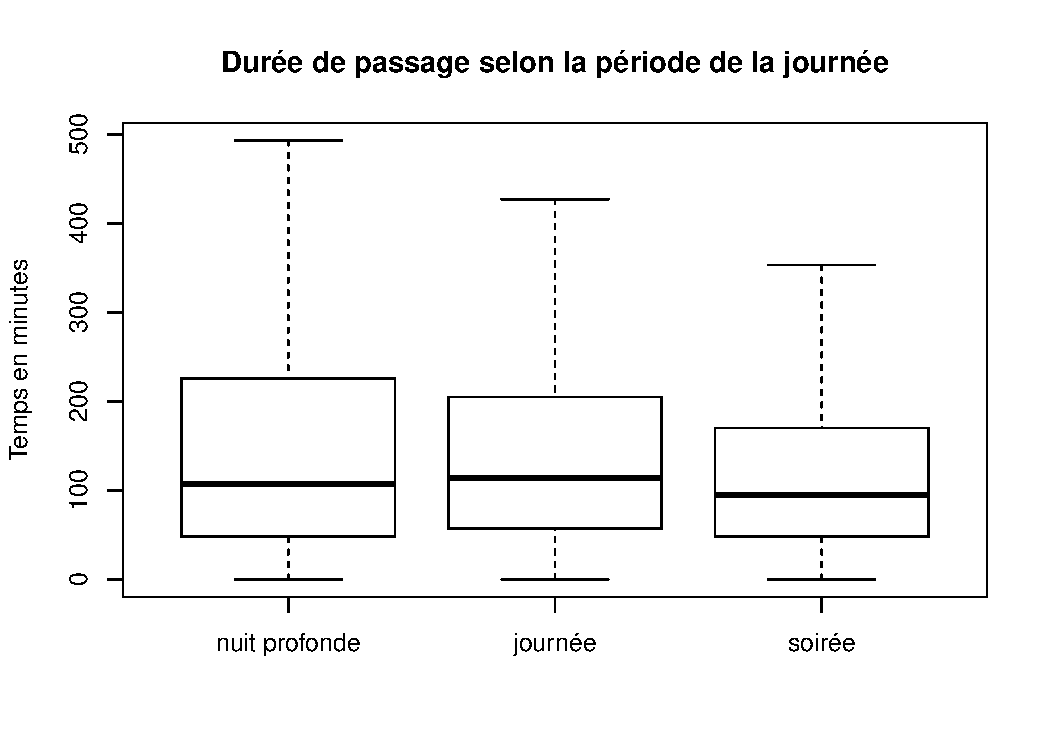
\includegraphics[width=\maxwidth]{figure/periode_2-1} 

\end{knitrout}
 \captionof{figure}{Passages selon la période de la journée}
 \label{fig:bp_periode2}
\end{center}


%\begin{figure}[ht!]
\begin{center}
\begin{knitrout}
\definecolor{shadecolor}{rgb}{0.969, 0.969, 0.969}\color{fgcolor}
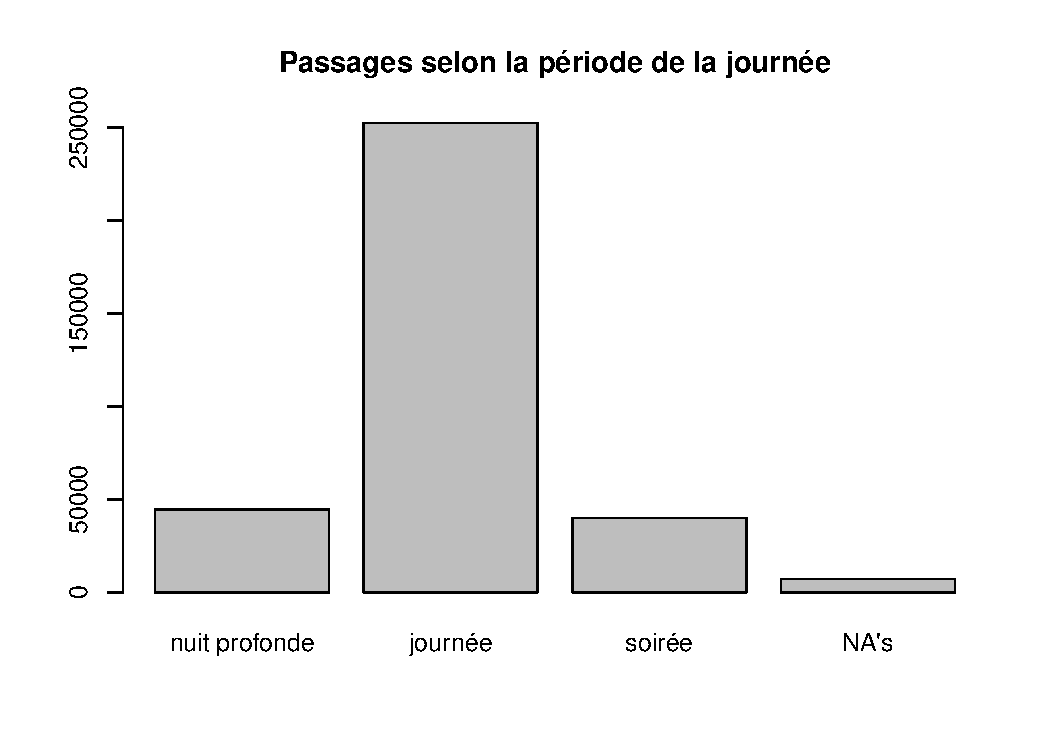
\includegraphics[width=\maxwidth]{figure/periode_1-1} 

\end{knitrout}
 \captionof{figure}{Passages selon la période de la journée}
 \label{fig:bp_periode1}
\end{center}

% latex table generated in R 3.1.2 by xtable 1.7-1 package
% Sat Nov  8 20:45:14 2014
\begin{table}[ht]
\centering
\begin{tabular}{rrrr}
  \hline
 & nuit profonde & journée & soirée \\ 
  \hline
mn & 182,30 & 160,60 & 157,96 \\ 
  \% & 36,40 & 32,06 & 31,54 \\ 
   \hline
\end{tabular}
\caption{Durée moyenne de présence pour le groupe b (10-1440 minutes)} 
\label{b_periode}
\end{table}


Durée moyenne de présence pour le groupe b (10-1440 minutes) (fig. \ref{b_periode} pp.\pageref{b_periode}).

%\begin{figure}[ht!]
\begin{center}
\begin{knitrout}
\definecolor{shadecolor}{rgb}{0.969, 0.969, 0.969}\color{fgcolor}
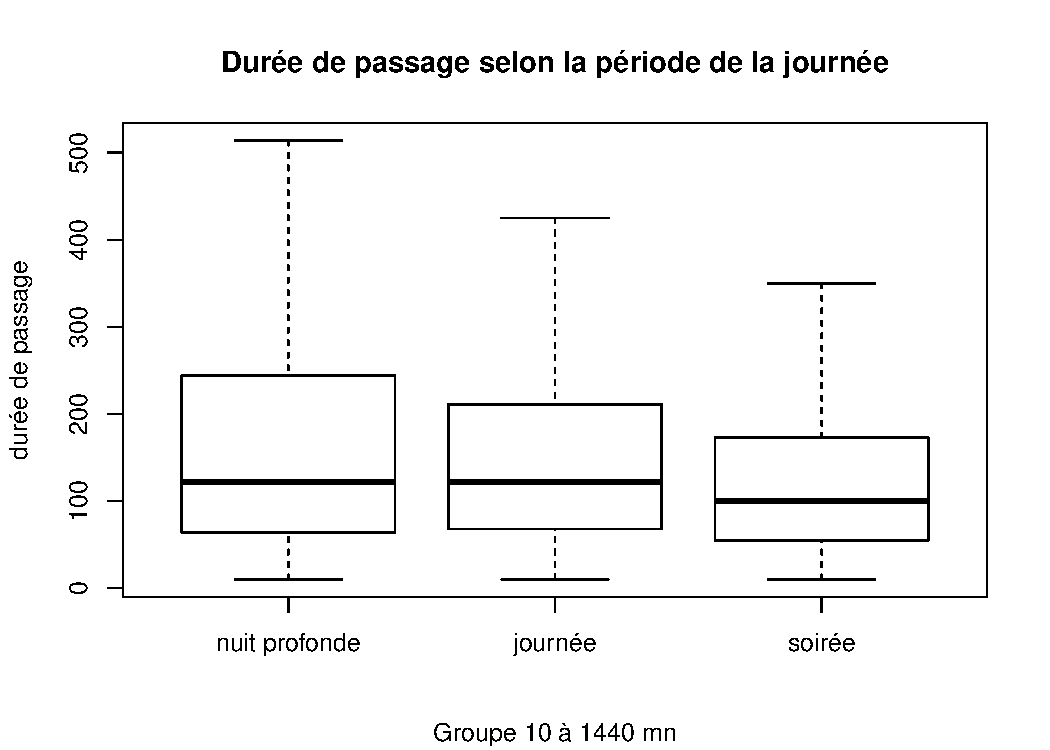
\includegraphics[width=\maxwidth]{figure/periode_4-1} 

\end{knitrout}
 \captionof{figure}{Passages selon la période de la journée}
\end{center}


% ************************
% *                      *  
% *     Selon l'age      * 
% *                      *
% ************************

\section{Selon l'âge}

On peut répartir les âges des patients en trois catégories (tableau \ref{tab:tranches_age} page \pageref{tab:tranches_age}). Le temps de passage augmente avec l'âge (table \ref{tab:age_dp} et figure \ref{fig:bp_age} page \pageref{fig:bp_age}).

% <<duree_age,echo=FALSE>>=
% #'@details utilisation de cut et split pour former des groupes d'age. CUT divise un groupe e valeurs x en différents intervalles. L'intervalle le plus à gauche correspond au niveau 1. Par défaut les intervalles sont fermés à droite. On met -1 comme borne inférieure pour inclure la valeur 0.

% latex table generated in R 3.1.2 by xtable 1.7-1 package
% Sat Nov  8 20:45:14 2014
\begin{table}[ht]
\centering
\begin{tabular}{rrrr}
  \hline
 & 15 ans et moins & 16 à 74 ans & 75 ans et plus \\ 
  \hline
n & 75 414,00 & 218 219,00 & 50 430,00 \\ 
  \% & 21,92 & 63,42 & 14,66 \\ 
   \hline
\end{tabular}
\caption[Répartition des RPU par tranches d'age]{Répartition des RPU par tranches d'age } 
\label{tab:tranches_age}
\end{table}



% latex table generated in R 3.1.2 by xtable 1.7-1 package
% Sat Nov  8 20:45:15 2014
\begin{table}[ht]
\centering
\begin{tabular}{rrrr}
  \hline
 & moyenne & ecart-type & médiane \\ 
  \hline
15 ans et moins & 113,33 & 125,95 & 85,00 \\ 
  16 à 74 ans & 168,17 & 199,09 & 116,00 \\ 
  75 ans et plus & 220,71 & 242,02 & 175,00 \\ 
   \hline
\end{tabular}
\caption[Durée de passage et age]{Durée de passage en fonction de l'âge} 
\label{tab:age_dp}
\end{table}


%\begin{figure}[ht!]
\begin{center}
\begin{knitrout}
\definecolor{shadecolor}{rgb}{0.969, 0.969, 0.969}\color{fgcolor}
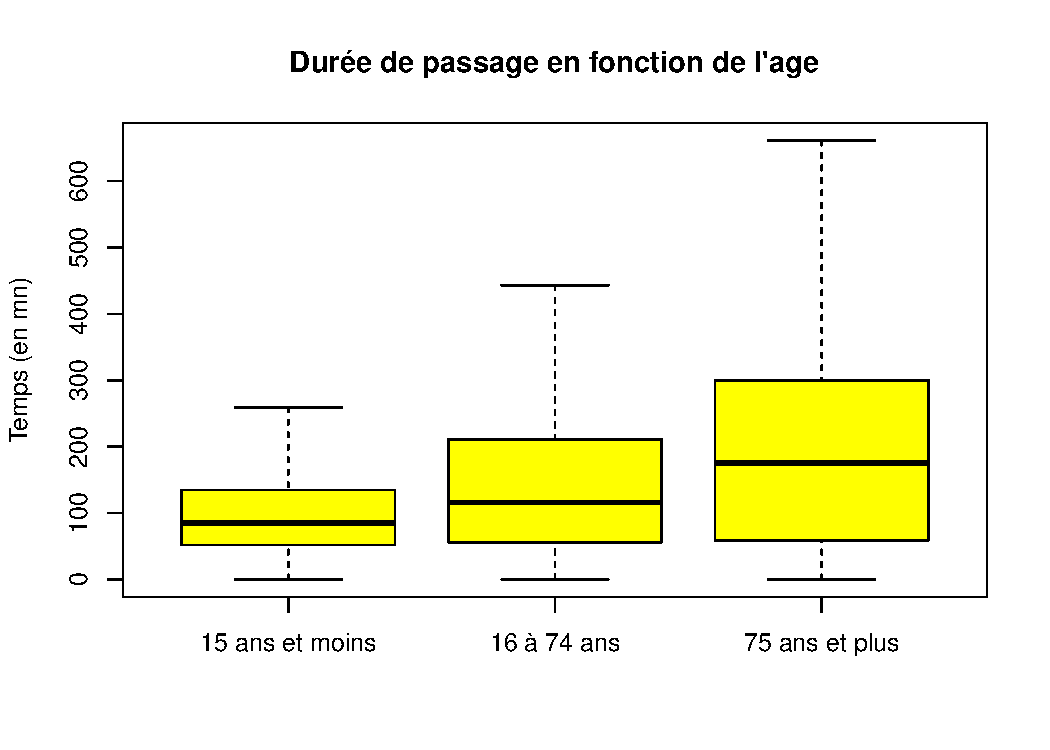
\includegraphics[width=\maxwidth]{figure/age_groupe2-1} 

\end{knitrout}
 \captionof{figure}{Durée de passage en fonction de l'âge}
 \label{fig:bp_age}
\end{center}

% *************************
% *                       *  
% * Selon le jour semaine * 
% *                       *
% *************************

\section{Selon le jour de la semaine}

% latex table generated in R 3.1.2 by xtable 1.7-1 package
% Sat Nov  8 20:45:15 2014
\begin{table}[ht]
\centering
\begin{tabular}{rrrrrrrr}
  \hline
 & Dim & Lun & Mar & Mer & Jeu & Ven & Sam \\ 
  \hline
mn & 149,85 & 171,44 & 166,78 & 162,48 & 163,29 & 163,99 & 161,35 \\ 
  \% & 13,15 & 15,05 & 14,64 & 14,26 & 14,33 & 14,40 & 14,16 \\ 
   \hline
\end{tabular}
\caption[Durée de présence et jour de la semaine]{Durée de présence et selon le jour de la semaine. Temps passé en minutes (mn) aux urgences en fonction du jour} 
\label{tab:jour_semaine}
\end{table}


Il existe une relation entre le jour de la semaine et la durée de présence aux urgences (table \ref{tab:jour_semaine} pp.\pageref{tab:jour_semaine}). La durée de présence est plus longue en début de semaine avec un maximum pour le lundi puis diminue progressivement pour atteindre un minimum le dimanche.

%\begin{figure}[ht!]
\begin{center}
\begin{knitrout}
\definecolor{shadecolor}{rgb}{0.969, 0.969, 0.969}\color{fgcolor}
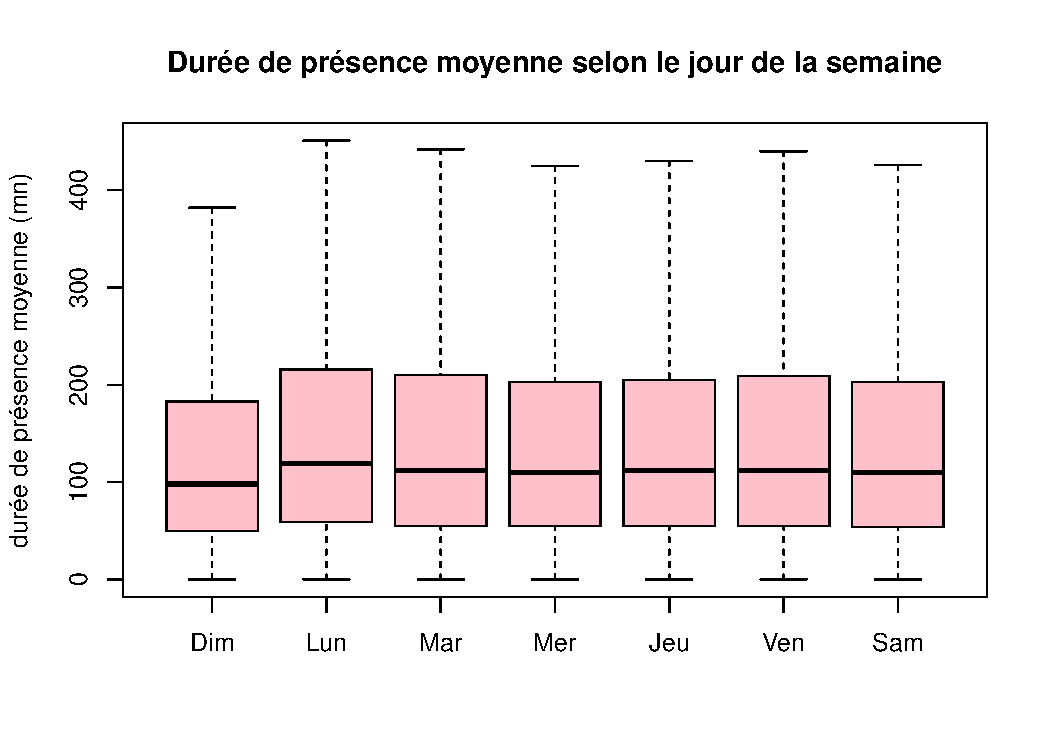
\includegraphics[width=\maxwidth]{figure/bp_jour_presence-1} 

\end{knitrout}
 \captionof{figure}{Durée de passage en fonction du jour de la semaine}
 \label{duree_jour}
\end{center}

Il existe une relation entre la destination et la durée de présence aux urgences (fig. \ref{duree_jour} pp.\pageref{duree_jour}).


% ************************
% *                      *  
% * Moins de 4 heures    * 
% *                      *
% ************************
\subsection{Pourcentage de passages en moins de 4 heures par établissement}



Pour l'ensemble des patients d'Alsace, 80\% d'entre eux quittent les urgences en moins de quatre heures.

% ************************
% *                      *  
% * Selon l'orientation  * 
% *                      *
% ************************

\section{Selon l'orientation}
% latex table generated in R 3.1.2 by xtable 1.7-1 package
% Sat Nov  8 20:45:16 2014
\begin{table}[ht]
\centering
\begin{tabular}{rrr}
  \hline
 & mn & \% \\ 
  \hline
REO & 86.25 & 3.24 \\ 
  UHCD & 88.99 & 3.34 \\ 
  SC & 167.79 & 6.31 \\ 
  PSA & 168.98 & 6.35 \\ 
  REA & 210.98 & 7.93 \\ 
  HO & 224.77 & 8.45 \\ 
  FUGUE & 228.88 & 8.60 \\ 
  HDT & 229.06 & 8.61 \\ 
  OBST & 234.94 & 8.83 \\ 
  CHIR & 239.33 & 9.00 \\ 
  SI & 253.45 & 9.53 \\ 
  MED & 262.76 & 9.88 \\ 
  SCAM & 264.29 & 9.93 \\ 
   \hline
\end{tabular}
\caption[Durée de présence et orientation]{Durée de présence et orientation. Temps passé en minutes (mn) aux urgences en fonction de l'orientation à l'issue de la prise en charge} 
\label{tab:duree_orientation}
\end{table}
% latex table generated in R 3.1.2 by xtable 1.7-1 package
% Sat Nov  8 20:45:16 2014
\begin{table}[ht]
\centering
\begin{tabular}{rrrrrrrr}
  \hline
 & DOM & HAD & HMS & MCO & PSY & SLD & SSR \\ 
  \hline
mn & 155,79 & 162,00 & 506,65 & 183,56 & 323,15 & 250,35 & 320,30 \\ 
  \% & 8,19 & 8,52 & 26,64 & 9,65 & 16,99 & 13,16 & 16,84 \\ 
   \hline
\end{tabular}
\caption[Durée de présence et destination]{Durée de présence et destination. Temps passé en minutes (mn) aux urgences en fonction de la destination à l'issue de la prise en charge} 
\label{tab:duree_destination}
\end{table}


Il existe une relation entre l'orientation et la durée de présence aux urgences (table \ref{tab:duree_orientation} pp.\pageref{tab:duree_orientation}).

Il existe une relation entre la destination et la durée de présence aux urgences (table \ref{tab:duree_destination} pp.\pageref{tab:duree_destination}).

%\begin{figure}[ht!]
\begin{center}
\begin{knitrout}
\definecolor{shadecolor}{rgb}{0.969, 0.969, 0.969}\color{fgcolor}
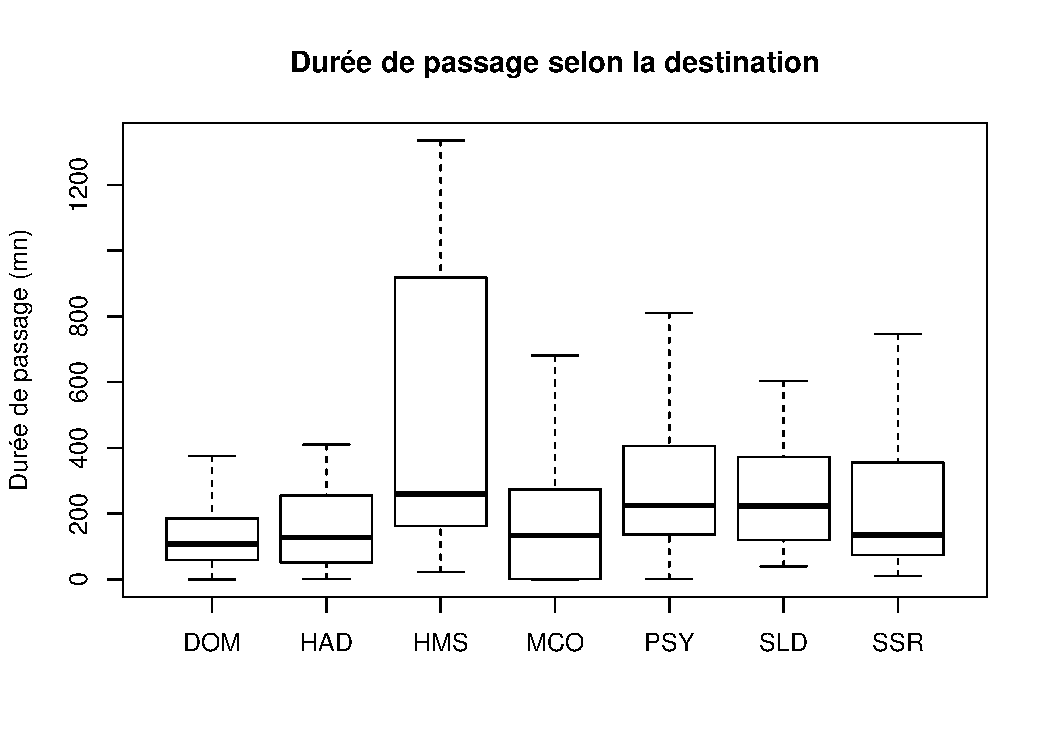
\includegraphics[width=\maxwidth]{figure/bp_duree_dest-1} 

\end{knitrout}
 \captionof{figure}{Durée de passage en fonction de la destination}
 \label{duree_dest}
\end{center}
Il existe une relation entre la destination et la durée de présence aux urgences (fig. \ref{duree_dest} pp.\pageref{duree_dest}).

% ************************
% *                      *  
% * Selon la gravité     * 
% *                      *
% ************************

\section{Selon la gravité}

% latex table generated in R 3.1.2 by xtable 1.7-1 package
% Sat Nov  8 20:45:16 2014
\begin{table}[ht]
\centering
\begin{tabular}{rrrrrrrr}
  \hline
 & 1 & 2 & 3 & 4 & 5 & D & P \\ 
  \hline
mn & 120,14 & 159,19 & 228,40 & 219,64 & 177,34 & 190,49 & 222,27 \\ 
  \% & 9,12 & 12,08 & 17,34 & 16,67 & 13,46 & 14,46 & 16,87 \\ 
   \hline
\end{tabular}
\caption[Durée de présence et gravité]{Durée de présence et gravité. Temps passé en minutes (mn) aux urgences en fonction de la CCMU} 
\label{duree_gravite}
\end{table}

Il existe une relation entre la gravité et la durée de présence aux urgences (table \ref{duree_gravite} pp.\pageref{duree_gravite}).

%\begin{figure}[ht!]
 \begin{center}
\begin{knitrout}
\definecolor{shadecolor}{rgb}{0.969, 0.969, 0.969}\color{fgcolor}
\includegraphics[width=\maxwidth]{figure/duree_gravite2-1} 

\end{knitrout}
 \captionof{figure}{Durée de passage en fonction de la gravité exprimée en unité CCMU}
 \label{toucan}
\end{center}


% ************************
% *                      *  
% * Selon la structure   * 
% *                      *
% ************************

\section{Selon la structure}

Voir les tableaux de bord de chaque établissement.

% \subsection{CH Sélestat}
% <<duree_structure,echo=FALSE>>=
% summary(sel$p)
% @
% 
% selon la gravité:
% <<duree_gravite_sel,echo=FALSE>>=
% tapply(sel$p,sel$GRAVITE,mean,na.rm=TRUE)
% @
% 
% selon l'orientation
% <<duree_orientation_sel,echo=FALSE>>=
% tapply(sel$p,sel$ORIENTATION,mean,na.rm=TRUE)
% 
% #'@details on transforme les NA en DOM pour mesurer le temps moyen si retour à domicile. On fait l'hypothèse que NA = dom.
% sel$DESTINATION<-as.character(sel$DESTINATION)
% sel$DESTINATION[is.na(sel$DESTINATION)]<-"DOM"
% tapply(sel$p,sel$DESTINATION,mean,na.rm=TRUE)
% @
% 
% A Sélestat, p\% des patients quittent les urgences en moins de quatre heures.
% 
% <<duree_semaine,echo=TRUE>>=
% tapply(sel$p,wday(e,label=TRUE),mean,na.rm=TRUE)
% # selon le jour et la période
% t<-table(periode,wday(e,label=TRUE))
% t
% @

% latex table generated in R 3.0.3 by xtable 1.7-3 package
% Sun Mar  9 17:20:02 2014

\newpage
\chapter{Codage diagnostique}

%



Les motifs de recours aux urgences sont exprimés en fonction de la classification CIM10 \cite{10}.
\index{motif de recours}
\footnote{Classification Internationale des Maladies, 10ème révision (La CIM10 comporte environ 36000 maladies).}.
\url{http://apps.who.int/classifications/icd10/browse/2008/fr}
Le fichier comporte \np{228 524} diagnostics principaux différents, 
répartis en 4 849 classes de diagnostics.
La comparaison entre le nombre de RPU reçus et le nombre de diagnostics renseignés permet d'établir l'exhaustivité des CIM10 à 66\% \index{exhaustivité!CIM10}


\section{CIM10}

Ventilation des diagnostics principaux en fonction des 22 chapitres de la CIM10. Le tableau qui suit indique pour chaque chapitre, le nombre total de cas rapportés, le pourcentage par rapport à l'ensemble, et le pourcentage de cas déduction faite de la traumatologie. En effet celle-ci représente environ la moitié des cas et il parait intéressant de séparer les pathologies traumatiques des non traumatiques.

\begin{knitrout}
\definecolor{shadecolor}{rgb}{0.969, 0.969, 0.969}\color{fgcolor}
\includegraphics[width=\maxwidth]{figure/table_cim10-1} 

\end{knitrout}


%round(prop.table(tr)*100,digits=2)

\begin{longtable}{|c|c|m{4cm}|c|c|c|}
 \hline
 Chapitre & Bloc & Titre & N & \% total  & \% non trauma \\
 \hline
 
I & A00–B99 & Certaines maladies infectieuses et parasitaires & 10 630 & 4.7 & 11 \\

 II&C00–D48&Tumeurs&1 076&0.47&1.1\\
 
III&D50–D89&Maladies du sang et des organes hématopoïétiques et certains troubles du système immunitaire&491&0.21&0.5\\

IV&E00–E90&Maladies endocriniennes, nutritionnelles et métaboliques&2 506&1.1&2.6\\

V&F00–F99&Troubles mentaux et du comportement&12 165&5.3&12\\

VI&G00–G99&Maladies du système nerveux&6 728&2.9&6.9\\

VII & H00–H59 & Maladies de l’œil et de ses annexes & 6 965 & 3&7.1\\

VIII&H60–H95&Maladies de l'oreille et de l'apophyse mastoïde&5 068&2.2&5.2\\

IX&I00–I99&Maladies de l'appareil circulatoire&13 740&6&14\\

X&J00–J99&Maladies de l'appareil respiratoire&24 257&11&25\\

XI&K00–K93&Maladies de l'appareil digestif&18 358&8&19\\

XII&L00–L99&Maladies de la peau et du tissu cellulaire sous cutané&6 929&3&7.1\\

XIII&M00–M99&Maladies du système ostéoarticulaire, des muscles et du tissu conjonctif&20 954&9.2&21\\

XIV&N00–N99&Maladies de l'appareil génito-urinaire&11 768&5.2&12\\

XV&O00–O99&Grossesse, accouchement et puerpéralité&417&0.18&0.43\\

XVI&P00–P96&Certaines affections dont l'origine se situe dans la période périnatale&396&0.17&0.4\\

% XVII&Q00–Q99&Malformations congénitales et anomalies chromosomiques&cong&round(cong*100/total,digits=2)&round(cong*100/(total-traumato),digits=2)\\

XVIII&R00–R99&Symptômes, signes et résultats anormaux d'examens cliniques et de laboratoire, non classés ailleurs&53 076&23&54\\

XIX&S00–T98&Lésions traumatiques, empoisonnements et certaines autres conséquences de causes externes&130 631&57& \\

XX&V01–Y98&Causes externes de morbidité et de mortalité& 6 184&2.7&6.3\\

XXI&Z00–Z99&Facteurs influant sur l'état de santé et motifs de recours aux services de santé&10 026&4.4&4.4\\

XXII&U00–U99&Codes d'utilisation particulière & 0&0&0\\

  \hline
\end{longtable}



\begin{knitrout}
\definecolor{shadecolor}{rgb}{0.969, 0.969, 0.969}\color{fgcolor}
\includegraphics[width=\maxwidth]{figure/class_cim10-1} 
\begin{kframe}\begin{verbatim}
classes.cim10 :  
        Fréquence Pourcentage Pourcentage cumul.
S           77664        34.0                 34
R           35297        15.4                 49
J           15661         6.9                 56
M           13972         6.1                 62
K           12249         5.4                 68
T            9286         4.1                 72
I            9036         4.0                 76
F            8138         3.6                 79
H            8025         3.5                 83
N            7885         3.5                 86
Z            6683         2.9                 89
A            4708         2.1                 91
L            4651         2.0                 93
G            4439         1.9                 95
B            2227         1.0                 96
W            1923         0.8                 97
E            1657         0.7                 98
D            1430         0.6                 98
Y             948         0.4                 99
X             711         0.3                 99
V             624         0.3                 99
C             522         0.2                100
O             282         0.1                100
P             257         0.1                100
r             130         0.1                100
Q              93         0.0                100
k              26         0.0                100
  Total    228524       100.0                100
\end{verbatim}
\end{kframe}
\end{knitrout}

%%%%%%%%%%%%%%%%%%%%%%%%%%%%%%%%%%%%%%
\section{Etude des AVC}
\index{AVC}
%%%%%%%%%%%%%%%%%%%%%%%%%%%%%%%%%%%%%

Les AVC sont définis par la nomenclature I60 à I64, G45 accidents ischémiques cérébraux transitoires (sauf G45.4 amnésie transitoire) et syndromes apparentés et G46 syndromes vasculaires cérébraux au cours de maladies cérébrovasculaires

La prévention et la prise en charge des accidents vasculaires cérébraux  Annexes 
juin 2009

Annexe : Liste exhaustive des codes CIM10 d’AVC
{\footnotesize
\begin{longtable}{|l|l|}
 \hline
 Code & libellé\\
 \hline
 G450 & Syndrome vertébrobasilaire \\
 G451 & Syndrome carotidien (hémisphérique) \\
 G452 & Accident ischémique transitoire de territoires artériels précérébraux multiples et bilatéraux \\
 G453 & Amaurose fugace \\
 G454 & Amnésie globale transitoire : NON RETENU \\
 G458 & Autres accidents ischémiques cérébraux transitoires et syndromes apparentés \\
 G459 & Accident ischémique cérébral transitoire, sans précision \\
 I600 & Hémorragie sousarachnoïdienne de la bifurcation et du siphon carotidien \\
 I601 & Hémorragie sousarachnoïdienne de l'artère cérébrale moyenne \\
 I602 & Hémorragie sousarachnoïdienne de l'artère communicante antérieure \\
 I603 & Hémorragie sousarachnoïdienne de l’artère communicante postérieure \\
 I604 & Hémorragie sousarachnoïdienne de l'artère basilaire \\
 I605 & Hémorragie sousarachnoïdienne de l'artère vertébrale \\
 I606 & Hémorragie sousarachnoïdienne d'autres artères intracrâniennes \\
 I607 & Hémorragie sousarachnoïdienne d'une artère intracrânienne, sans précision \\
 I608 & Autres hémorragies sous arachnoïdiennes \\
 I609 & Hémorragie sousarachnoïdienne, sans précision \\
 I610 & Hémorragie intracérébrale hémisphérique, sous corticale \\
 I611 & Hémorragie intracérébrale hémisphérique, corticale \\
 I612 & Hémorragie intracérébrale hémisphérique, non précisée \\
 I613 & Hémorragie intracérébrale du tronc cérébral \\
 I614 & Hémorragie intracérébrale cérébelleuse \\
 I615 & Hémorragie intracérébrale intraventriculaire \\
 I616 & Hémorragie intracérébrale,localisations multiples \\
 I618 & Autres hémorragies intracérébrales \\
 I619 & Hémorragie intracérébrale, sans précision \\
 I620 & Hémorragie sousdurale (aiguë) (non traumatique) \\
 I621 & Hémorragie extradurale non traumatique \\
 I629 & Hémorragie intracrânienne (non traumatique), sans précision \\
 I630 & Infarctus cérébral dû à une thrombose des artères précérébrales \\
 I631 & Infarctus cérébral dû à une embolie des artères précérébrales \\
 I632 & Infarctus cérébral dû à une occlusion ou sténose des artères précérébrales,de mécanisme non précisé \\
 I633 & Infarctus cérébral dû à une thrombose des artères cérébrales \\
 I634 & Infarctus cérébral dû à une embolie des artères cérébrales \\
 I635 & Infarctus cérébral dû à une occlusion ou sténose des artères cérébrales, de mécanisme non précisé \\
 I636 & Infarctus cérébral dû à une thrombose veineuse cérébrale, non pyogène \\
 I638 & Autres infarctus cérébraux \\
 I639 & Infarctus cérébral, sans précision \\
 I64 & Accident vasculaire cérébral, non précisé comme étant hémorragique ou par infarctus \\
 G460 & Syndrome de l'artère cérébrale moyenne (I66.0) (1) \\
 G461 & Syndrome de l'artère cérébrale antérieure (I66.1) (1) \\
 G462 & Syndrome de l'artère cérébrale postérieure (I66.2) (1) \\
 G463 & Syndromes vasculaires du tronc cérébral (I60I67) (1) \\
 G464 & Syndrome cérébelleux vasculaire (I60I67) (1) \\
 G465 & Syndrome lacunaire moteur pur (I60I67) (1) \\
 G466 & Syndrome lacunaire sensitif pur (I60I67) (1) \\
 G467 & Autres syndromes lacunaires (I60I67) (1) \\
 G468 & Autres syndromes vasculaires cérébraux au cours de maladies cérébrovasculaires (I60I67) (1) \\
  \hline
\end{longtable}
} % end small



%-----------------------------
\subsection*{Horaire des AVC}
%-----------------------------

\index{AVC!heure}

Horaire des AVC, à comparer avec:
\begin{itemize}
  \item les crises d'épilepsie
  \item la pression atmosphérique
\end{itemize}

\begin{figure}[ht!]
 \centering
\begin{knitrout}
\definecolor{shadecolor}{rgb}{0.969, 0.969, 0.969}\color{fgcolor}
\includegraphics[width=\maxwidth]{figure/heure_avc-1} 

\end{knitrout}
 \caption{Horaire de survenue des AVC}
 \label{fig:horaire_avc}
\end{figure}


\begin{knitrout}
\definecolor{shadecolor}{rgb}{0.969, 0.969, 0.969}\color{fgcolor}
\includegraphics[width=\maxwidth]{figure/heure_avc2-1} 

\end{knitrout}

% latex table generated in R 3.1.2 by xtable 1.7-1 package
% Sat Nov  8 20:45:18 2014
\begin{table}[ht]
\centering
\begin{tabular}{rrrr}
  \hline
 & Fréquence & Pourcentage & Pourcentage cumul. \\ 
  \hline
0 & 45,00 & 1,60 & 1,60 \\ 
  1 & 38,00 & 1,40 & 3,00 \\ 
  2 & 35,00 & 1,20 & 4,20 \\ 
  3 & 29,00 & 1,00 & 5,20 \\ 
  4 & 17,00 & 0,60 & 5,90 \\ 
  5 & 26,00 & 0,90 & 6,80 \\ 
  6 & 25,00 & 0,90 & 7,70 \\ 
  7 & 49,00 & 1,80 & 9,40 \\ 
  8 & 100,00 & 3,60 & 13,00 \\ 
  9 & 173,00 & 6,20 & 19,20 \\ 
  10 & 238,00 & 8,50 & 27,70 \\ 
  11 & 246,00 & 8,80 & 36,50 \\ 
  12 & 200,00 & 7,10 & 43,60 \\ 
  13 & 175,00 & 6,20 & 49,90 \\ 
  14 & 201,00 & 7,20 & 57,00 \\ 
  15 & 172,00 & 6,10 & 63,20 \\ 
  16 & 181,00 & 6,50 & 69,60 \\ 
  17 & 197,00 & 7,00 & 76,70 \\ 
  18 & 171,00 & 6,10 & 82,80 \\ 
  19 & 129,00 & 4,60 & 87,40 \\ 
  20 & 150,00 & 5,40 & 92,80 \\ 
  21 & 80,00 & 2,90 & 95,60 \\ 
  22 & 68,00 & 2,40 & 98,00 \\ 
  23 & 55,00 & 2,00 & 100,00 \\ 
    Total & 2 800,00 & 100,00 & 100,00 \\ 
   \hline
\end{tabular}
\caption[Horaire de passage des AVC]{Horaires de passages des AVC en 2013.} 
\label{fig:passage_avc}
\end{table}



%-----------------------------------------
\subsection*{Selon le jour de la semaine}
%-----------------------------------------

\index{AVC!jour de la semaine}

% latex table generated in R 3.1.2 by xtable 1.7-1 package
% Sat Nov  8 20:45:18 2014
\begin{table}[ht]
\centering
\begin{tabular}{rrrrrrrr}
  \hline
 & Lun & Mar & Mer & Jeu & Ven & Sam & Dim \\ 
  \hline
fréquence & 467.00 & 457.00 & 399.00 & 396.00 & 408.00 & 350.00 & 323.00 \\ 
  p.cent & 16.68 & 16.32 & 14.25 & 14.14 & 14.57 & 12.50 & 11.54 \\ 
   \hline
\end{tabular}
\caption[AVC selon le jour de la semaine]{Distribution des AVC en fonction du jour de la semaine. La fréquence quotidienne théorique est de 14.28 p.cent d'AVC par jour. Les AvC sont plus fréquents en début de semainet plus rares en fin de semaine.} 
\label{tab:avc_jour}
\end{table}

\includegraphics[width=\maxwidth]{figure/avc_jour_semaine-1} 

Proportion théorique = 14.28\% par jour de la semaine.

%------------------------
\subsection*{AVC et âge}
%------------------------

\index{AVC!âge}
% latex table generated in R 3.1.2 by xtable 1.7-1 package
% Sat Nov  8 20:45:18 2014
\begin{table}[ht]
\centering
\begin{tabular}{rrrrrrr}
  \hline
 & moyenne & écart-type & médiane & min & max & n \\ 
  \hline
1 & 71.40 & 16.18 & 75.00 & 1.00 & 112.00 & 2800.00 \\ 
   \hline
\end{tabular}
\end{table}

Le rapport de 2009 donne âge moyen = 70.5 et âge médian = 75 ans. La population alsacienne, vue sous l'angle des RPU, semble se distribuer comme la population française.

\begin{knitrout}
\definecolor{shadecolor}{rgb}{0.969, 0.969, 0.969}\color{fgcolor}
\includegraphics[width=\maxwidth]{figure/avc_age2-1} 

\includegraphics[width=\maxwidth]{figure/avc_age2-2} 

\end{knitrout}



%------------------------
\subsection*{AVC et sexe}
%------------------------

\index{AVC!sexe}

% latex table generated in R 3.1.2 by xtable 1.7-1 package
% Sat Nov  8 20:45:18 2014
\begin{table}[ht]
\centering
\begin{tabular}{rrr}
  \hline
 & Femmes & Hommes \\ 
  \hline
n & 1 476,00 & 1 324,00 \\ 
  \% & 52,71 & 47,29 \\ 
   \hline
\end{tabular}
\caption[AVC et sexe]{Répartition des AVC entre les hommes et les femmes} 
\label{tab:sr_avc}
\end{table}


Le \textbf{sexe-ratio} est égal à \textbf{0.9}, traduisant une prédominance féminine (table \ref{tab:sr_avc}).

\begin{knitrout}
\definecolor{shadecolor}{rgb}{0.969, 0.969, 0.969}\color{fgcolor}
\includegraphics[width=\maxwidth]{figure/avc_sexe2-1} 

\includegraphics[width=\maxwidth]{figure/avc_sexe2-2} 

\end{knitrout}

%%%%%%%%%%%%%%%%%%%%%%%%%%%%%%%%%%%%%%%%%%%%%%%%%%%
\section{Accidents ischémiques transitoires (AIT)}
\index{AIT}
%%%%%%%%%%%%%%%%%%%%%%%%%%%%%%%%%%%%%%%%%%%%%%%%%%%

Recommandations pour la sélection des données PMSI MCO concernant l’AVC (Juin 2009)

{\small
\begin{longtable}{|l|l|}
 \hline
 Code & libellé\\
 \hline
G450 & Syndrome vertébro-basilaire \\
G451 & Syndrome carotidien (hémisphérique) \\
G452 & Accident ischémique transitoire de territoires artériels précérébraux multiples et bilatéraux \\
G453  & Amaurose fugace \\
G458  & Autres accidents ischémiques cérébraux transitoires et syndromes apparentés \\
G459  & Accident ischémique cérébral transitoire, sans précision \\  
  \hline
\end{longtable}
} % end small

Le thésaurus SFMU (2013) \cite{9} recommande d'utiliser G45.9 (ou G459) pour tout diagnostic d'AIT.
\index{AIT!thésaurus}


\includegraphics[width=\maxwidth]{figure/ait-1} 
% latex table generated in R 3.1.2 by xtable 1.7-1 package
% Sat Nov  8 20:45:18 2014
\begin{table}[ht]
\centering
\begin{tabular}{rrrr}
  \hline
 & Fréquence & Pourcentage & Pourcentage cumul. \\ 
  \hline
G450 & 4,00 & 0,60 & 0,60 \\ 
  G451 & 7,00 & 1,00 & 1,60 \\ 
  G452 & 20,00 & 2,80 & 4,40 \\ 
  G453 & 7,00 & 1,00 & 5,40 \\ 
  G458 & 52,00 & 7,40 & 12,70 \\ 
  G459 & 617,00 & 87,30 & 100,00 \\ 
    Total & 707,00 & 100,00 & 100,00 \\ 
   \hline
\end{tabular}
\caption[Types d'AIT]{Distribution des AIT en 2013.} 
\label{tab:ait}
\end{table}


%%%%%%%%%%%%%%%%%%%%%%%%%%%%%
\section{Pneumonies}
\index{pneumonies}
%%%%%%%%%%%%%%%%%%%%%%%%%%%%

% latex table generated in R 3.1.2 by xtable 1.7-1 package
% Sat Nov  8 20:45:18 2014
\begin{table}[ht]
\centering
\begin{tabular}{rrrrrrr}
  \hline
 & moyenne & écart-type & médiane & min & max & n \\ 
  \hline
âge & 70.87 & 19.41 & 77.00 & 0.00 & 98.00 & 841.00 \\ 
   \hline
\end{tabular}
\caption[Pneumonies et âge]{Pneumonies et âge} 
\label{tab:pneumo_age}
\end{table}


Les pneumopathies bactériennes sans précision sont cotées J15.9 Dans la CIM10.
841 diagnostics de ce type ont été portés au SAU en 2013.

Les pneumonies bactériennes concernent les adultes âgés des deux sexes. L'âge moyen est de 71 ans et la moitié de ces patients ont 77 ans et plus (table \ref{tab:pneumo_age} pp.\pageref{tab:pneumo_age}).

\begin{knitrout}
\definecolor{shadecolor}{rgb}{0.969, 0.969, 0.969}\color{fgcolor}
\includegraphics[width=\maxwidth]{figure/pneumo-1} 

\end{knitrout}

En fonction de la gravité (CCMU):

\includegraphics[width=\maxwidth]{figure/unnamed-chunk-40-1} 
% latex table generated in R 3.1.2 by xtable 1.7-1 package
% Sat Nov  8 20:45:18 2014
\begin{table}[ht]
\centering
\begin{tabular}{rrrr}
  \hline
 & Fréquence & Pourcentage & \% hors NA's \\ 
  \hline
1 & 16.00 & 1.90 & 1.90 \\ 
  2 & 359.00 & 42.70 & 43.30 \\ 
  3 & 390.00 & 46.40 & 47.00 \\ 
  4 & 57.00 & 6.80 & 6.90 \\ 
  5 & 8.00 & 1.00 & 1.00 \\ 
  D & 0.00 & 0.00 & 0.00 \\ 
  P & 0.00 & 0.00 & 0.00 \\ 
  NA's & 11.00 & 1.30 & 0.00 \\ 
    Total & 841.00 & 100.00 & 100.00 \\ 
   \hline
\end{tabular}
\caption[Gravité des pneumonies]{Gravité des pneumonies chez les patients ayant consulté un  SU, en région Alsace en 2013} 
\label{tab:pneumonies}
\end{table}


En fonction de la destination: table \ref{tab:pneumo_dest}

% latex table generated in R 3.1.2 by xtable 1.7-1 package
% Sat Nov  8 20:45:18 2014
\begin{table}[ht]
\centering
\begin{tabular}{rrrr}
  \hline
 & Fréquence & Pourcentage & \% hors NA's \\ 
  \hline
NA & 0.00 & 0.00 & 0.00 \\ 
  MCO & 624.00 & 74.20 & 99.40 \\ 
  SSR & 1.00 & 0.10 & 0.20 \\ 
  SLD & 0.00 & 0.00 & 0.00 \\ 
  PSY & 3.00 & 0.40 & 0.50 \\ 
  HAD & 0.00 & 0.00 & 0.00 \\ 
  HMS & 0.00 & 0.00 & 0.00 \\ 
  NA's & 213.00 & 25.30 & 0.00 \\ 
    Total & 841.00 & 100.00 & 100.00 \\ 
   \hline
\end{tabular}
\caption[Pneumonies et service d'hospitalisation]{Destination des patients admis pour pneumonie aux urgences en région Alsace en 2013} 
\label{tab:pneumo_dest}
\end{table}


En fonction de l'orientation: table \ref{tab:pneumo_orient}

% latex table generated in R 3.1.2 by xtable 1.7-1 package
% Sat Nov  8 20:45:18 2014
\begin{table}[ht]
\centering
\begin{tabular}{rrrr}
  \hline
 & Fréquence & Pourcentage & \% hors NA's \\ 
  \hline
CHIR & 13.00 & 1.50 & 2.30 \\ 
  FUGUE & 0.00 & 0.00 & 0.00 \\ 
  HDT & 0.00 & 0.00 & 0.00 \\ 
  HO & 0.00 & 0.00 & 0.00 \\ 
  MED & 280.00 & 33.30 & 50.20 \\ 
  OBST & 0.00 & 0.00 & 0.00 \\ 
  PSA & 0.00 & 0.00 & 0.00 \\ 
  REA & 11.00 & 1.30 & 2.00 \\ 
  REO & 0.00 & 0.00 & 0.00 \\ 
  SC & 5.00 & 0.60 & 0.90 \\ 
  SCAM & 0.00 & 0.00 & 0.00 \\ 
  SI & 2.00 & 0.20 & 0.40 \\ 
  UHCD & 247.00 & 29.40 & 44.30 \\ 
  NA's & 283.00 & 33.70 & 0.00 \\ 
    Total & 841.00 & 100.00 & 100.00 \\ 
   \hline
\end{tabular}
\caption[Pneumonies et service d'hospitalisation]{Orientation des patients admis pour pneumonie aux urgences en région Alsace en 2013} 
\label{tab:pneumo_orient}
\end{table}


Des patients porteurs de problèmes respiratoires sont orientés en chirurgie : erreur ou manque de place en médecine ?

%%%%%%%%%%%%%%%%%%%%%%%%%%%
\section{Syndrome grippal}
\index{syndrome grippal}
%%%%%%%%%%%%%%%%%%%%%%%%%%%

\begin{knitrout}
\definecolor{shadecolor}{rgb}{0.969, 0.969, 0.969}\color{fgcolor}
\includegraphics[width=\maxwidth]{figure/grippe-1} 

\end{knitrout}

%%%%%%%%%%%%%%%%%%%%%%%%%%%%%%%
\section{Asthme}
\index{Asthme}
%%%%%%%%%%%%%%%%%%%%%%%%%%%%%%%

Classification selon la CIM10:
\begin{itemize}
  \item J45.0 Asthme à prédominance allergique
  \item J45.1 Asthme non allergique
  \item J45.8 Asthme associé 
  \item J45.9 Asthme, sans précision
  \item J46   Etat de mal asthmatique
\end{itemize}

% latex table generated in R 3.1.2 by xtable 1.7-1 package
% Sat Nov  8 20:45:18 2014
\begin{table}[ht]
\centering
\begin{tabular}{rr}
  \hline
 & V1 \\ 
  \hline
J450 & 133 \\ 
  J451 & 205 \\ 
  J458 &   8 \\ 
  J459 & 999 \\ 
  J46 &  53 \\ 
   \hline
\end{tabular}
\caption[]{Diagnostics d'asthme} 
\end{table}

\includegraphics[width=\maxwidth]{figure/asthme-1} 
% latex table generated in R 3.1.2 by xtable 1.7-1 package
% Sat Nov  8 20:45:18 2014
\begin{table}[ht]
\centering
\begin{tabular}{rrrr}
  \hline
 & Fréquence & Pourcentage & Pourcentage Cumul. \\ 
  \hline
J458 & 8.00 & 0.60 & 0.60 \\ 
  J46 & 53.00 & 3.80 & 4.40 \\ 
  J450 & 133.00 & 9.50 & 13.90 \\ 
  J451 & 205.00 & 14.70 & 28.50 \\ 
  J459 & 999.00 & 71.50 & 100.00 \\ 
    Total & 1398.00 & 100.00 & 100.00 \\ 
   \hline
\end{tabular}
\caption[Répartition des diagnostics d'asthme]{Répartition des diagnostics d'asthme chez les patients ayant consulté un  SU, en région Alsace en 2013} 
\label{tab:asthme}
\end{table}


On note \np{1 398} cas d'asthme en 2013.


\includegraphics[width=\maxwidth]{figure/asthme2-1} 

\includegraphics[width=\maxwidth]{figure/asthme2-2} 
% latex table generated in R 3.1.2 by xtable 1.7-1 package
% Sat Nov  8 20:45:18 2014
\begin{table}[ht]
\centering
\begin{tabular}{rrrr}
  \hline
 & Fréquence & Pourcentage & Pourcentage cumul. \\ 
  \hline
1 & 26.00 & 1.90 & 1.90 \\ 
  2 & 21.00 & 1.50 & 3.40 \\ 
  3 & 32.00 & 2.30 & 5.70 \\ 
  4 & 23.00 & 1.60 & 7.30 \\ 
  5 & 27.00 & 1.90 & 9.20 \\ 
  6 & 21.00 & 1.50 & 10.70 \\ 
  7 & 28.00 & 2.00 & 12.70 \\ 
  8 & 22.00 & 1.60 & 14.30 \\ 
  9 & 23.00 & 1.60 & 16.00 \\ 
  10 & 21.00 & 1.50 & 17.50 \\ 
  11 & 41.00 & 2.90 & 20.40 \\ 
  12 & 23.00 & 1.60 & 22.00 \\ 
  13 & 25.00 & 1.80 & 23.80 \\ 
  14 & 27.00 & 1.90 & 25.80 \\ 
  15 & 22.00 & 1.60 & 27.30 \\ 
  16 & 40.00 & 2.90 & 30.20 \\ 
  17 & 41.00 & 2.90 & 33.10 \\ 
  18 & 27.00 & 1.90 & 35.10 \\ 
  19 & 34.00 & 2.40 & 37.50 \\ 
  20 & 37.00 & 2.60 & 40.10 \\ 
  21 & 41.00 & 2.90 & 43.10 \\ 
  22 & 26.00 & 1.90 & 44.90 \\ 
  23 & 47.00 & 3.40 & 48.30 \\ 
  24 & 31.00 & 2.20 & 50.50 \\ 
  25 & 29.00 & 2.10 & 52.60 \\ 
  26 & 14.00 & 1.00 & 53.60 \\ 
  27 & 25.00 & 1.80 & 55.40 \\ 
  28 & 17.00 & 1.20 & 56.60 \\ 
  29 & 11.00 & 0.80 & 57.40 \\ 
  30 & 15.00 & 1.10 & 58.40 \\ 
  31 & 13.00 & 0.90 & 59.40 \\ 
  32 & 19.00 & 1.40 & 60.70 \\ 
  33 & 13.00 & 0.90 & 61.70 \\ 
  34 & 14.00 & 1.00 & 62.70 \\ 
  35 & 8.00 & 0.60 & 63.20 \\ 
  36 & 17.00 & 1.20 & 64.40 \\ 
  37 & 50.00 & 3.60 & 68.00 \\ 
  38 & 37.00 & 2.60 & 70.70 \\ 
  39 & 33.00 & 2.40 & 73.00 \\ 
  40 & 20.00 & 1.40 & 74.50 \\ 
  41 & 26.00 & 1.90 & 76.30 \\ 
  42 & 22.00 & 1.60 & 77.90 \\ 
  43 & 26.00 & 1.90 & 79.80 \\ 
  44 & 22.00 & 1.60 & 81.30 \\ 
  45 & 25.00 & 1.80 & 83.10 \\ 
  46 & 44.00 & 3.10 & 86.30 \\ 
  47 & 32.00 & 2.30 & 88.60 \\ 
  48 & 30.00 & 2.10 & 90.70 \\ 
  49 & 28.00 & 2.00 & 92.70 \\ 
  50 & 26.00 & 1.90 & 94.60 \\ 
  51 & 24.00 & 1.70 & 96.30 \\ 
  52 & 45.00 & 3.20 & 99.50 \\ 
  53 & 7.00 & 0.50 & 100.00 \\ 
    Total & 1398.00 & 100.00 & 100.00 \\ 
   \hline
\end{tabular}
\caption[Fréquence des crises d'asthme]{Fréquence des crises d'asthme par semaine en 2013} 
\label{tab:freq_asthme}
\end{table}



La population des patients consultant pour une crise d’asthme est jeune (voir table \ref{tab:age_asthme} page \pageref{tab:age_asthme}).

\begin{center}
\begin{knitrout}
\definecolor{shadecolor}{rgb}{0.969, 0.969, 0.969}\color{fgcolor}
\includegraphics[width=\maxwidth]{figure/asthme_age-1} 

\end{knitrout}
\captionof{figure}{Histogramme des classes d'âge pour l'asthme.}\label{fig:asthme_age}%
\end{center}

\begin{center}
\begin{knitrout}
\definecolor{shadecolor}{rgb}{0.969, 0.969, 0.969}\color{fgcolor}
\includegraphics[width=\maxwidth]{figure/asthme_ccmu-1} 

\end{knitrout}
\captionof{figure}{Gravité des crises d'asthme.}\label{fig:asthme_ccmu}%
\end{center}

[[1]]
NULL

[[2]]
[1] "moyenne"    "écart-type" "médiane"    "min"        "max"       
[6] "n"         

% latex table generated in R 3.1.2 by xtable 1.7-1 package
% Sat Nov  8 20:45:18 2014
\begin{table}[ht]
\centering
\begin{tabular}{rrrrrrr}
  \hline
 & moyenne & écart-type & médiane & min & max & n \\ 
  \hline
1 & 22.85 & 23.80 & 13.00 & 0.00 & 97.00 & 1398.00 \\ 
   \hline
\end{tabular}
\caption[Asthme et âge]{Âge de la population consultant pour crise d'asthme} 
\label{tab:age_asthme}
\end{table}
% latex table generated in R 3.1.2 by xtable 1.7-1 package
% Sat Nov  8 20:45:18 2014
\begin{table}[ht]
\centering
\begin{tabular}{rrrrrrrrr}
  \hline
 & 1 & 2 & 3 & 4 & 5 & D & P & NA's \\ 
  \hline
1 & 150 & 880 & 325 &  24 &   5 &   0 &   0 &  14 \\ 
   \hline
\end{tabular}
\caption[Asthme et CCMU]{Gravité de la crise d'asthme en fonction de la CCMU} 
\label{tab:ccmu_asthme}
\end{table}


Les crises sont de gravité moyenne avec une prédominance de CCMU 2 et 3 (voir table \ref{tab:ccmu_asthme} page \pageref{tab:ccmu_asthme}).
Cependant le taux d'hospitalisation est important: 38 \%.
\np{88} patients ont été orientés vers un service "chaud" (Réanimation, soins intensifs ou continus) soit 19 \% des patients hospitalisés pour asthme.

Le bulletin épidémiologique (Le point épidémiologique du 24 octobre 2013 - Surveillance épidémiologique de la Cire Lorraine-Alsace) clôt la surveillance de l’asthme. Pour l’association SOS Médecins de Strasbourg, l’activité liée à l’asthme a été particulièrement marquée de mi-avril (semaine 16) à fin mai(semaine 22) puis en semaine 40. Concernant l’association de Mulhouse, seule une forte augmentation en semaine 39 a été observée depuis début avril.

%%%%%%%%%%%%%%%%%%%%%%%%%%%%
\section{Bronchiolite}
\index{Bronchiolite}
%%%%%%%%%%%%%%%%%%%%%%%%%%%%

CIM10: Bronchiolite aiguë

Inclus:
    avec bronchospasme
\begin{itemize}
  \item J21.0 Bronchiolite aiguë due au virus respiratoire syncytial [VRS]
  \item J21.8 Bronchiolite aiguë due à d'autres micro-organismes précisés
  \item J21.9 Bronchiolite aiguë, sans précision
\end{itemize}

\begin{knitrout}
\definecolor{shadecolor}{rgb}{0.969, 0.969, 0.969}\color{fgcolor}
\includegraphics[width=\maxwidth]{figure/bron-1} 

\includegraphics[width=\maxwidth]{figure/bron-2} 

\end{knitrout}

Sur représentation de Mulhouse. 
Taux hospitalisation: 50\%


%%%%%%%%%%%%%%%%%%%%%%%%%%%%
\section{Intoxication au CO}
\index{Intoxication au CO}
%%%%%%%%%%%%%%%%%%%%%%%%%%%%

CIM10 = T58

\begin{knitrout}
\definecolor{shadecolor}{rgb}{0.969, 0.969, 0.969}\color{fgcolor}\begin{kframe}
\begin{verbatim}
Jan Fev Mar Avr Mai Jun Jui Aou Sep Oct Nov Dec 
  5  13  11   0   6   9   0   1   1   1  15   4 
\end{verbatim}
\end{kframe}
\includegraphics[width=\maxwidth]{figure/co-1} 

\end{knitrout}


%%%%%%%%%%%%%%%%%%%%%%%%%%%%
\section{Malaises}
\index{malaise}
%%%%%%%%%%%%%%%%%%%%%%%%%%%%

Cette rubrique associe les codes suivants:

\begin{itemize}
  \item \textbf{R55}: syncope, lipothymie, malaise vagal
  \item \textbf{R53}: altération de l'état général, fatigue, épuisement
  \item \textbf{R42}: étourdissement, vertiges
\end{itemize}

\subsection*{Malaise de type vagal (R55)}

\begin{knitrout}
\definecolor{shadecolor}{rgb}{0.969, 0.969, 0.969}\color{fgcolor}
\includegraphics[width=\maxwidth]{figure/malaises-1} 

\end{knitrout}

\subsection*{malaise selon INVS (canicule)}

Regroupe tous les intitulés: R55, R53 et R42.

\begin{knitrout}
\definecolor{shadecolor}{rgb}{0.969, 0.969, 0.969}\color{fgcolor}
\includegraphics[width=\maxwidth]{figure/malaises_invs-1} 

\end{knitrout}

%%%%%%%%%%%%%%%%%%%%%%%%%%%%%%%
\section{Marqueurs de canicule}
\index{Canicule@marqueurs}
%%%%%%%%%%%%%%%%%%%%%%%%%%%%%%%

Données hospitalières : nombre quotidien de passages dans des services d'urgence hospitaliers pour un diagnostic de malaise (codes CIM10 R42, R53 et R55), d'hyperthermie et autres effets directs de la chaleur (codes CIM10 T67 et X30), de déshydratation (code CIM10 E86) et d'hyponatrémie (code CIM10 E871)

- X30  Exposition à une chaleur naturelle excessive
- E86  Déplétion du volume du plasma ou du liquide extra cellulaire, Déshydratation sauf choc hypovolémique

\begin{knitrout}
\definecolor{shadecolor}{rgb}{0.969, 0.969, 0.969}\color{fgcolor}
\includegraphics[width=\maxwidth]{figure/canicule-1} 

\includegraphics[width=\maxwidth]{figure/canicule-2} 
\begin{kframe}\begin{verbatim}
canicule : 
        Fréquence Pourcentage Pourcentage cumul.
T670           57        73.1                 73
T671            8        10.3                 83
T672            3         3.8                 87
T676            2         2.6                 90
T677            6         7.7                 97
T678            1         1.3                 99
T679            1         1.3                100
  Total        78       100.0                100
\end{verbatim}
\end{kframe}
\includegraphics[width=\maxwidth]{figure/canicule-3} 

\end{knitrout}

%%%%%%%%%%%%%%%%%%%%%%%%%%%%%%%
\section{Gastro-entérites}
\index{Gastroentérites}
%%%%%%%%%%%%%%%%%%%%%%%%%%%%%%%

CIM10 \textbf{A09} : Diarrhée et gastro-entérite d'origine présumée infectieuse. Les RPU retournent 3 codes: A09, A090 et A099 correspondant à la classification CIM10-PMSI:
\begin{itemize}
  \item \textbf{A090} Gastroentérites et colites d’origine infectieuse, autres et non précisées
  \item \textbf{A099} Gastroentérites et colites d’origine non précisée
\end{itemize}

Inclus: Catarrhe intestinale (Colite,Entérite, Gastro-entérite,SAI hémorragique,septique), Diarrhée (SAI,dysentérique,épidémique), Maladie diarrhéique infectieuse SAI.
Sont exclues: diarrhée non infectieuse (K52.9), néonatale (P78.3), maladies dues à des bactéries, des protozoaires, des virus et d'autres agents infectieux précisés (A00-A08) 



\subsection*{Une pathologie de l'enfant et de l'adulte jeune}


\begin{itemize}
  \item age moyen 18 ans.
  \item age médian 5 ans.
  \item 75\% des paients ont moins de 27 ans.
\end{itemize}

\begin{knitrout}
\definecolor{shadecolor}{rgb}{0.969, 0.969, 0.969}\color{fgcolor}

{\centering \includegraphics[width=\maxwidth]{figure/ge_hist-1} 

}



\end{knitrout}

\begin{knitrout}
\definecolor{shadecolor}{rgb}{0.969, 0.969, 0.969}\color{fgcolor}

{\centering \includegraphics[width=\maxwidth]{figure/ge_age_box-1} 

}



\end{knitrout}

\subsection*{Epidémiologie des gastro-entérites}

\begin{knitrout}
\definecolor{shadecolor}{rgb}{0.969, 0.969, 0.969}\color{fgcolor}
\includegraphics[width=\maxwidth]{figure/ge_epidemio-1} 

\end{knitrout}

% calculs à la manière de l'INVS
\subsection*{nombre de diagnostics de GE par rapport au nombre total de RPU par semaine}

\begin{knitrout}
\definecolor{shadecolor}{rgb}{0.969, 0.969, 0.969}\color{fgcolor}\begin{kframe}
\begin{verbatim}
                     Jan     Fev     Mar     Avr      Mai      Jun
RPU totaux       18392.0 18052.0 19523.0 20302.0 19207.00 20772.00
Gastro-entérites   306.0   240.0   264.0   282.0   181.00   168.00
Rapport              1.7     1.3     1.4     1.4     0.94     0.81
                      Jui     Aou      Sep      Oct      Nov     Dec
RPU totaux       20387.00 19275.0 18272.00 18519.00 17387.00 18436.0
Gastro-entérites   173.00   219.0   174.00   165.00   149.00   360.0
Rapport              0.85     1.1     0.95     0.89     0.86     1.9
\end{verbatim}
\end{kframe}
\end{knitrout}

\begin{knitrout}
\definecolor{shadecolor}{rgb}{0.969, 0.969, 0.969}\color{fgcolor}

{\centering \includegraphics[width=\maxwidth]{figure/invs_barplot-1} 

}



\end{knitrout}


\begin{knitrout}
\definecolor{shadecolor}{rgb}{0.969, 0.969, 0.969}\color{fgcolor}\begin{kframe}
\begin{verbatim}
##      
##        A09 A090 A099
##   3Fr    0   50  178
##   Alk    0   15   35
##   Col  302   43   18
##   Dia    0    0    0
##   Geb    0   27  123
##   Hag    0   40   21
##   Hus    0   46   31
##   Mul 1411    0    0
##   Odi    0   13   35
##   Sel    0   61   62
##   Wis    0   81   89
##   Sav    0    0    0
\end{verbatim}
\end{kframe}
\end{knitrout}

%%%%%%%%%%%%%%%%%%%%%%%%%%%%%%%
\section{Traumatologie}
\index{Traumatologie}
%%%%%%%%%%%%%%%%%%%%%%%%%%%%%%%

% dpt: tous les cas de traumato (S00 à T98)
% dpnt:tous les cas de médecine  


% latex table generated in R 3.1.2 by xtable 1.7-1 package
% Sat Nov  8 20:45:20 2014
\begin{table}[ht]
\centering
\begin{tabular}{rrrrrr}
  \hline
 & RPU médicaux & Traumatologie & Ratio med/trauma & Trauma ratio & Med ratio \\ 
  \hline
Jan & 11 670 & 6 722 & 2 & 0 & 1 \\ 
  Fev & 11 891 & 6 161 & 2 & 0 & 1 \\ 
  Mar & 12 170 & 7 353 & 2 & 0 & 1 \\ 
  Avr & 12 812 & 7 490 & 2 & 0 & 1 \\ 
  Mai & 11 411 & 7 796 & 1 & 0 & 1 \\ 
  Jun & 12 152 & 8 620 & 1 & 0 & 1 \\ 
  Jui & 12 326 & 8 061 & 2 & 0 & 1 \\ 
  Aou & 11 792 & 7 483 & 2 & 0 & 1 \\ 
  Sep & 11 006 & 7 266 & 2 & 0 & 1 \\ 
  Oct & 11 478 & 7 041 & 2 & 0 & 1 \\ 
  Nov & 10 901 & 6 486 & 2 & 0 & 1 \\ 
  Dec & 11 965 & 6 471 & 2 & 0 & 1 \\ 
   \hline
\end{tabular}
\caption[RPU traumatiques]{Comparaison de la fréquence des RPU d'origine traumatique et non traumatique.} 
\label{tab:trauma}
\end{table}


La classification CIM 10 range dans la catégorie de traumatologie, les codes S00 à T98. Les autres codes rassemblent les RPU non traumatiques ou médicaux (table \ref{tab:trauma} page \pageref{tab:trauma}). Le ratio moyen entre les RPU traumatiques et non traumatiques (trauma ratio) est de 0.38.

\subsection{Age et traumatologie}

Les patients consultant pour de la traumatologie sont plus jeunes que ceux consultant pour une autre cause. L'age moyen est de 34 ans pour la traumatologie contre 43 ans pour les RPU médicaux. 


\includegraphics[width=\maxwidth]{figure/trauma_age-1} 


Cette différence est statistiquement significative (p = 0).

\begin{itemize}
  \item Nombre de cas de traumatologie: 86 950
  \item Nombre de cas médicaux: 141 574
  \item Trauma ratio moyen: 0.38
  \item Med ratio moyen: 0.62
\end{itemize}



 

\newpage
\chapter{Modalités de sortie}

% sortie.Rnw

\section{Mode de sortie}
\index{Mode de sortie}

Le RPU connaît trois mode de sortie des urgences:
\begin{enumerate}
  \item le décès: le patient est déclaré décédé aux urgences.
  \item le retour à domicile ou ce qui en tient lieu (y compris la voie publique)
  \item l'hospitalisation (mutation ou transfert)
  \begin{itemize}
  \item mutation: le patient est hospitalisé dans une autre unité médicale de la même entité juridique sauf pour les établissements privés visés aux alinéas d et e de l'article L162-22-6 du code de la sécurité sociale.
  \item transfert: le patient est hospitalisé dans une autre  entité juridique sauf pour les établissements privés visés aux alinéas d et e de l'article L162-22-6 du code de la sécurité sociale.
\end{itemize}
\end{enumerate}

% Mode de SORTIE.png: 669x437 pixel, 72dpi, 23.60x15.42 cm, bb=0 0 669 437
 \begin{figure}[h]
 \centering
 \includegraphics[width=9cm,height=7cm,bb=0 0 669 437]{figure/Mode de SORTIE.png}
 \caption{Modes de sortie}
\end{figure}

% latex table generated in R 3.1.2 by xtable 1.7-1 package
% Sat Nov  8 20:45:21 2014
\begin{table}[ht]
\centering
\begin{tabular}{|l|r|r|}
  \hline
 & n & \% \\ 
  \hline
Décès & 2 & 0.00 \\ 
  Domicile & 223155 & 64.86 \\ 
  Mutation & 68191 & 19.82 \\ 
  $<$NA$>$ & 47767 & 13.88 \\ 
  Transfert & 4958 & 1.44 \\ 
   \hline
\end{tabular}
\caption[Mode de sortie des urgences]{Mode de sortie des urgences. <NA> est le nombre de non réponses à cet item} 
\label{tab.sortie}
\end{table}


\section{Mode de sortie selon la structure}

Les données par établissement sont résumées dans le tableau \ref{tab.sortie_etab} page \pageref{tab.sortie_etab}

% latex table generated in R 3.1.2 by xtable 1.7-1 package
% Sat Nov  8 20:45:21 2014
\begin{table}[ht]
\centering
\begin{tabular}{|l|r|r|r|r|r|r|}
  \hline
 & Décès & Domicile & Mutation & $<$NA$>$ & Transfert & Sum \\ 
  \hline
3Fr & 0.00 & 90.99 & 1.50 & 7.38 & 0.12 & 99.99 \\ 
  Alk & 0.00 & 81.10 & 15.01 & 1.61 & 2.28 & 100.00 \\ 
  Col & 0.00 & 73.07 & 23.12 & 1.97 & 1.84 & 100.00 \\ 
  Dia & 0.00 & 82.19 & 10.04 & 7.14 & 0.62 & 99.99 \\ 
  Geb & 0.00 & 51.30 & 2.09 & 45.31 & 1.30 & 100.00 \\ 
  Hag & 0.00 & 56.44 & 23.97 & 15.08 & 4.52 & 100.01 \\ 
  Hus & 0.00 & 2.14 & 54.94 & 42.92 & 0.00 & 100.00 \\ 
  Mul & 0.00 & 61.88 & 14.23 & 23.66 & 0.23 & 100.00 \\ 
  Odi & 0.00 & 93.85 & 0.00 & 1.78 & 4.38 & 100.01 \\ 
  Sel & 0.01 & 78.81 & 21.16 & 0.02 & 0.00 & 100.00 \\ 
  Wis & 0.00 & 75.65 & 22.45 & 0.62 & 1.27 & 99.99 \\ 
  Sav & 0.00 & 69.14 & 19.37 & 10.42 & 1.08 & 100.01 \\ 
   \hline
\end{tabular}
\caption[Mode de sortie selon l'établissement]{Mode de sortie des urgences selon l'établissement (en pourcentage). <NA> est le nombre de non réponses à cet item} 
\label{tab.sortie_etab}
\end{table}



\section{Orientation}
\index{orientation}

Le mode de sortie est affiné par la rubrique ORIENTATION avec la ventilation suivante:

\begin{itemize}
  \item NA:    Pas d'informations
  \item MCO:		Hospitalisation conventionnelle
  \item SSR:		Soins de suite et de réadaptation
  \item SLD:		Soins de longue durée
  \item PSY: 		Psychiatrie
  \item HAD:		Hospitalisation à domicile
  \item HMS:		Hébergement médico-social
\end{itemize}

On notera que le retour à domicile proprement dit ne figure pas parmi les items et cette modalité est implicite. On peut supposer que les NA's correspondent à cette modalité. Cependant une ambiguité demeure car les non réponses sont aussi représentées par ce symbole.

a
  CHIR  FUGUE    HDT     HO    MED   OBST    PSA    REA    REO     SC 
  7872    260    126     31  18522     98   3126   1035   1446   1426 
  SCAM     SI   UHCD   <NA> 
   522   1402  32452 275755 
% latex table generated in R 3.1.2 by xtable 1.7-1 package
% Sat Nov  8 20:45:21 2014
\begin{table}[ht]
\centering
\begin{tabular}{rrrrrrrr}
  \hline
 & 1 & 2 & 3 & 4 & 5 & D & P \\ 
  \hline
NA &   0 &   0 &   0 &   0 &   0 &   0 &   0 \\ 
  MCO & 2379 & 27301 & 29223 & 2826 & 701 &  10 & 143 \\ 
  SSR &   1 &  68 &  31 &   2 &   0 &   0 &   0 \\ 
  SLD &   1 &  10 &  13 &   2 &   0 &   0 &   0 \\ 
  PSY &  61 & 271 & 157 &  12 &   9 &   0 & 613 \\ 
  HAD &   0 &   4 &   2 &   0 &   0 &   0 &   0 \\ 
  HMS &   3 &  15 &   2 &   0 &   0 &   0 &   0 \\ 
   \hline
\end{tabular}
\caption[Destination et gravité]{Destination et gravité (la gravité est exprimée en unités CCMU)} 
\label{tab:dest_gravite}
\end{table}
% latex table generated in R 3.1.2 by xtable 1.7-1 package
% Sat Nov  8 20:45:21 2014
\begin{table}[ht]
\centering
\begin{tabular}{rrrrrrrr}
  \hline
 & 1 & 2 & 3 & 4 & 5 & D & P \\ 
  \hline
CHIR & 181 & 3331 & 3662 & 363 &  11 &   1 & 140 \\ 
  FUGUE &  67 & 141 &  22 &   0 &   0 &   0 &   9 \\ 
  HDT &   4 &  30 &  24 &   1 &   0 &   0 &  48 \\ 
  HO &   0 &  16 &   5 &   0 &   0 &   0 &  10 \\ 
  MED & 827 & 5966 & 9670 & 704 &  39 &   1 & 274 \\ 
  OBST &   3 &  53 &  35 &   3 &   0 &   0 &   0 \\ 
  PSA & 1109 & 558 &  32 &   0 &   0 &   0 &   8 \\ 
  REA &   1 &  99 & 246 & 266 & 408 &   0 &   3 \\ 
  REO & 955 & 349 &  52 &   0 &   0 &   0 &   1 \\ 
  SC &  80 & 419 & 749 & 138 &  24 &   0 &   9 \\ 
  SCAM &  77 & 324 &  81 &   3 &   0 &   0 &   2 \\ 
  SI &  19 & 319 & 757 & 255 &  29 &   0 &   2 \\ 
  UHCD & 1258 & 12752 & 9190 & 1157 & 191 &   7 &  48 \\ 
   \hline
\end{tabular}
\caption[Orientation et gravité]{Orientation et gravité (la gravité est exprimée en unités CCMU). Certaines orientations sont curieuses: CCMU1 ou 2 et Réanimation, CCMU 5 et services de médecine ou de chirurgie.} 
\label{tab:orient_gravite}
\end{table}


\section{Destination}
\index{destination}
% latex table generated in R 3.1.2 by xtable 1.7-1 package
% Sat Nov  8 20:45:21 2014
\begin{table}[ht]
\centering
\begin{tabular}{rr}
  \hline
 & \% \\ 
  \hline
HAD & 0.01 \\ 
  HMS & 0.03 \\ 
  MCO & 98.18 \\ 
  PSY & 1.61 \\ 
  SLD & 0.04 \\ 
  SSR & 0.14 \\ 
   \hline
\end{tabular}
\caption{Destination des patients non rentrés à domicile après leur passage aux urgences} 
\label{tab.dest.hosp}
\end{table}
% latex table generated in R 3.1.2 by xtable 1.7-1 package
% Sat Nov  8 20:45:21 2014
\begin{table}[ht]
\centering
\begin{tabular}{rr}
  \hline
 & \% \\ 
  \hline
DOM & 78.79 \\ 
  HAD & 0.00 \\ 
  HMS & 0.01 \\ 
  MCO & 20.82 \\ 
  PSY & 0.34 \\ 
  SLD & 0.01 \\ 
  SSR & 0.03 \\ 
   \hline
\end{tabular}
\caption{Devenir des patients à la sortie des urgences. DOM représentent ceux qui sont repartis vers leur domicile ou ce qui en tient lieu (sous l'hypothèse que toutes les non réponses correspondent à un retour à domicile).} 
\label{tab.dest}
\end{table}


\section{Incohérences}

\index{Incohérences}

On isole le groupe "mode de sortie = domicile" et on relève les résultats de l'item "orientation" correspondant à ce groupe:


\includegraphics[width=\maxwidth]{figure/fausses_sorties-1} 
% latex table generated in R 3.1.2 by xtable 1.7-1 package
% Sat Nov  8 20:45:21 2014
\begin{table}[ht]
\centering
\begin{tabular}{rrrr}
  \hline
 & Fréquence & Pourcentage & Pourcentage cumulé \\ 
  \hline
NA's & 265 103,00 & 97,90 & 0,00 \\ 
  PSA & 3 074,00 & 1,10 & 52,80 \\ 
  REO & 1 402,00 & 0,50 & 24,10 \\ 
  SCAM & 522,00 & 0,20 & 9,00 \\ 
  UHCD & 283,00 & 0,10 & 4,90 \\ 
  FUGUE & 259,00 & 0,10 & 4,50 \\ 
  CHIR & 134,00 & 0,00 & 2,30 \\ 
  MED & 73,00 & 0,00 & 1,30 \\ 
  SI & 36,00 & 0,00 & 0,60 \\ 
  HDT & 16,00 & 0,00 & 0,30 \\ 
  REA & 10,00 & 0,00 & 0,20 \\ 
  SC & 6,00 & 0,00 & 0,10 \\ 
  HO & 2,00 & 0,00 & 0,00 \\ 
  OBST & 2,00 & 0,00 & 0,00 \\ 
    Total & 270 922,00 & 100,00 & 100,00 \\ 
   \hline
\end{tabular}
\caption[Orientation des patients non hospitalisés]{Orientation des patients non hospitalisés. Certaines orientations sont incompatibles avec un retour à domicile (Défaut de cohérence).} 
\label{tab:orient_nh}
\end{table}


Certaines orientations sont incompatibles avec un retour à domicile:
\begin{itemize}
  \item HO
  \item Obstétrique
  \item Soins continus, soins intensifs et réanimation
  \item UHCD, médecine et chirurgie
  
\end{itemize}



\newpage
\chapter{Modalités d'orientation}

% orientation.Rnw

\index{orientation}

Le mode d'orientation au sens du RPU est une rubrique un peu fourre-tout regroupant des hospitalisations comme des sorties "anormales" de la filière de soins (fugues, sortie contre avis, etc.).

\newpage
\chapter{Courbes d'activité régionale}

% activite_su.Rnw
% Courbe d'activité régionale
\index{Activité régionale}
 
%note\footnote{activite_su_Rnw}

\section{Variation du nombre total de passages journaliers}
\index{Passages@journaliers}


\includegraphics[width=\maxwidth]{figure/passages_totaux-1} 
% latex table generated in R 3.1.2 by xtable 1.7-1 package
% Sat Nov  8 20:45:22 2014
\begin{table}[ht]
\centering
\begin{tabular}{rrrrrrrrrrr}
  \hline
 & n & Min & Q25 & Moyenne & E-type & Médiane & Q75 & Max & Na & \%Na \\ 
  \hline
 & 364,00 & 675,00 & 897,00 & 945,30 & 86,30 & 949,00 & 997,20 & 1 182,00 & 0,00 & 0,00 \\ 
   \hline
\end{tabular}
\caption[Passages totaux]{Nombre de RPU transmis quotidiennement en 2013. Principaux paramètres statistiques.} 
\label{tab:pt}
\end{table}



\section{Variation du pourcentage journalier de retour à domicile}

\index{Retour à domicile}

Le nombre de retours à domicile est obtenu à partir de la rubrique MODE\_SORTIE. Il s'agit en fait des patients qui n'ont pas été hospitalisés. Sont également comptabilisés dans cette rubrique les sorties atypiques.

Les variations du retour journalier à domicile sont calculées de la manière suivante:
\begin{description}
  \item[numérateur] somme quotidienne où MODE\_SORTIE = Domicile
  \item[dénominateur] somme quotidienne des ENTREE (correspond à q)
\end{description}

% latex table generated in R 3.1.2 by xtable 1.7-1 package
% Sat Nov  8 20:45:23 2014
\begin{table}[ht]
\centering
\begin{tabular}{rrrrrrrrrrr}
  \hline
 & n & Min & Q25 & Moyenne & E-type & Médiane & Q75 & Max & Na & \%Na \\ 
  \hline
 & 364,00 & 57,50 & 62,40 & 64,80 & 3,40 & 64,50 & 66,80 & 77,20 & 0,00 & 0,00 \\ 
   \hline
\end{tabular}
\caption[Retour à domicile]{Pourcentage de retours à domicile - patients n'ayant été ni hospitalisés, ni transférés dans un autre établissement. Ce taux est plus faible en début d'année, lorsque les épisodes de tension sont plus fréquents.} 
\label{tab:rd}
\end{table}

\includegraphics[width=\maxwidth]{figure/retour_dom-1} 


On refait le calcul de q en tenant compte des non réponses:
% latex table generated in R 3.1.2 by xtable 1.7-1 package
% Sat Nov  8 20:45:24 2014
\begin{table}[ht]
\centering
\begin{tabular}{rrrrrrrrrrr}
  \hline
 & n & Min & Q25 & Moyenne & E-type & Médiane & Q75 & Max & Na & \%Na \\ 
  \hline
 & 364,00 & 67,00 & 73,00 & 75,20 & 3,00 & 75,10 & 77,20 & 82,70 & 0,00 & 0,00 \\ 
   \hline
\end{tabular}
\caption[Retours à domicile sans les non réponses]{Retours à domicile sans les non réponses (en pourcentage du nombre de RPU renseignés)} 
\label{tab:rdsansNA}
\end{table}

\includegraphics[width=\maxwidth]{figure/retour_dom2-1} 


Si on considère que tout ce qui n'est pas un retour à domicile constitue une hospitalisation, on peut tracer un graphique, miroir du précédent. La ligne bleue représente la moyenne lissée sur sept jours. On notera le taux d'hospitalisation élévé du début de l'année, correspondant à une période de forte tension. Les fluctuations de ce paramètre (comme le retour à domicile) sont une piste intéressante dans le cadre de la recherche d'indicateurs d'hôpital en tension, cependant les seuils d'alerte (triggers) restent à déterminer.

% latex table generated in R 3.1.2 by xtable 1.7-1 package
% Sat Nov  8 20:45:24 2014
\begin{table}[ht]
\centering
\begin{tabular}{rrrrrrrrrrr}
  \hline
 & n & Min & Q25 & Moyenne & E-type & Médiane & Q75 & Max & Na & \%Na \\ 
  \hline
 & 364,00 & 0,20 & 0,20 & 0,20 & 0,00 & 0,20 & 0,30 & 0,30 & 0,00 & 0,00 \\ 
   \hline
\end{tabular}
\caption[Hospitalisations]{Hospitalisations (ou transferts) sans les non réponses. En moyenne NA des passages entraînent une hospitalisation.} 
\label{tab:hosp}
\end{table}

\includegraphics[width=\maxwidth]{figure/hospit-1} 



% latex table generated in R 3.1.2 by xtable 1.7-1 package
% Sat Nov  8 20:45:24 2014
\begin{table}[ht]
\centering
\begin{tabular}{rrrrrrrrrrr}
  \hline
 & n & Min & Q25 & Moyenne & E-type & Médiane & Q75 & Max & Na & \%Na \\ 
  \hline
 & 364,00 & 0,80 & 0,80 & 0,90 & 0,00 & 0,90 & 0,90 & 1,00 & 0,00 & 0,00 \\ 
   \hline
\end{tabular}
\caption[Activité des SU et non réponses]{Activité des SU et non réponses - dans environ 13.84 \% des cas, on ne sait pas ce que devient le patient.} 
\label{tab:NAsu}
\end{table}

\includegraphics[width=\maxwidth]{figure/retour_dom3-1} 


%Le taux de réponse pour cet item est de `r round(q6 * 100, 2)` \%.

\index{exhaustivité@mode de sortie}

% ************************
% *                      *  
% *      PARTIE 3        * 
% *                      *
% ************************
\part{Analyse thématique} 
\newpage

\chapter{Pédiatrie}

% pediatrie.Rnw
\index{Pédiatrie}
\label{chap_pediatrie}



Les moins de 18 ans représentent $83 455$ passages en 2013 soit $230$ passages par jour.

% nombre de passages en fonction de l'age

\begin{knitrout}
\definecolor{shadecolor}{rgb}{0.969, 0.969, 0.969}\color{fgcolor}
\includegraphics[width=\maxwidth]{figure/passages_pediatrie-1} 

\end{knitrout}

% Pédiatrie et sexe

% latex table generated in R 3.1.2 by xtable 1.7-1 package
% Sat Nov  8 20:45:25 2014
\begin{table}[ht]
\centering
\begin{tabular}{rrr}
  \hline
 & F & M \\ 
  \hline
n & 37314.00 & 46127.00 \\ 
  \% & 44.72 & 55.28 \\ 
   \hline
\end{tabular}
\caption[Sex-ratio en pédiatrie]{Sex-ratio en pédiatrie} 
\label{tab:ped_sr}
\end{table}


Le sex-ratio est de $1.2$ (table \ref{tab:ped_sr})

% Taux hospitalisation

% latex table generated in R 3.1.2 by xtable 1.7-1 package
% Sat Nov  8 20:45:25 2014
\begin{table}[ht]
\centering
\begin{tabular}{rrrr}
  \hline
 & Hospitalisation & Domicile & Décès \\ 
  \hline
n & 7701.00 & 68640.00 & 0.00 \\ 
  \% & 10.09 & 89.91 & 0.00 \\ 
   \hline
\end{tabular}
\caption[Devenir du patient pédiatrique]{Devenir du patient pédiatrique} 
\label{tab:ped_hosp}
\end{table}


Le taux d'hospitalisation est de : \textbf{$10$ \%} (table \ref{tab:ped_hosp}).

% Durée de présence



\begin{itemize}
  \item Durée de présence moyenne: $118$ minutes soit 1:58 heures.
  \item Durée de présence médiane: $87$ minutes.
  \item Durée de présence la plus longue: $4.3$ jours.
\end{itemize}

\subsubsection*{Entrée - sorties pediatriques}

\begin{knitrout}
\definecolor{shadecolor}{rgb}{0.969, 0.969, 0.969}\color{fgcolor}
\includegraphics[width=\maxwidth]{figure/es_pediatriques-1} 

\end{knitrout}

\chapter{Gériatrie}

% geriatrie.Rnw

\index{Gériatrie}
\label{chap_geriatrie}



Les 75 ans et plus représentent $53 081$ passages en 2013 soit $146$ passages par jour.

% nombre de passages en fonction sde l'age

\begin{knitrout}
\definecolor{shadecolor}{rgb}{0.969, 0.969, 0.969}\color{fgcolor}
\includegraphics[width=\maxwidth]{figure/passages_geriatrie-1} 

\end{knitrout}

% Gériatrie et sexe

% latex table generated in R 3.1.2 by xtable 1.7-1 package
% Sat Nov  8 20:45:26 2014
\begin{table}[ht]
\centering
\begin{tabular}{rrr}
  \hline
 & F & M \\ 
  \hline
n & 32277.00 & 20793.00 \\ 
  \% & 60.82 & 39.18 \\ 
   \hline
\end{tabular}
\caption[Sex-ratio en gériatrie]{Sex-ratio en gériatrie} 
\label{tab:ger_sr}
\end{table}


\index{sex-ratio!en gériatrie}

Le sex-ratio est de $0.64$

% Taux d'hospitalisation

% latex table generated in R 3.1.2 by xtable 1.7-1 package
% Sat Nov  8 20:45:26 2014
\begin{table}[ht]
\centering
\begin{tabular}{rrrr}
  \hline
 & Hospitalisation & Domicile & Décès \\ 
  \hline
n & 26840.00 & 16585.00 & 1.00 \\ 
  \% & 61.81 & 38.19 & 0.00 \\ 
   \hline
\end{tabular}
\end{table}


Le taux d'hospitalisation est de $62$ \%.

% Durée de présence



\begin{itemize}
  \item Durée de présence moyenne: $275$ minutes soit 4:35 heures.
  \item Durée de présence médiane: $220$ minutes.
  \item Durée de présence la plus longue: $3$ jours.
\end{itemize}

Note: on ne retient que les durées de présence supérieures à 30 minutes.

\subsubsection*{Entrée - sorties gériatriques}

\begin{knitrout}
\definecolor{shadecolor}{rgb}{0.969, 0.969, 0.969}\color{fgcolor}
\includegraphics[width=\maxwidth]{figure/es_geriatriques-1} 

\end{knitrout}



% ************************
% *                      *  
% *      PARTIE 4        * 
% *                      *
% ************************
\part{Activité par service d'urgence}
\label{partie4}

\newpage

\chapter{SU Wissembourg}

% Su_Wissembourg.Rnw

\index{SU Wissembourg}
\index{CH de Wissembourg!SU}



% \pm dessine le symboe plus ou moins
% a["age_min"] donne une date que R n'arrive pas à utiliser. On utilise a[1,2] à la place

\begin{tabular}{|l|c|}
\hline 
\multicolumn{2}{|c|}{SU de Wissembourg}\tabularnewline
\hline 
\hline 
RPU déclarés & \np{12 646} \tabularnewline
\hline 
Date de début & 2 013-01-01 01:11:00 \tabularnewline
\hline 
Date de fin & 2 013-12-31 23:33:00 \tabularnewline
\hline 
Age moyen & 43 ans $\pm 27$ \tabularnewline
\hline 
RPU pédiatriques & \np{3 202} (25 \%) \tabularnewline
\hline 
RPU gériatriques & \np{2 190} (17 \%) \tabularnewline
\hline 
Durée de passage moyenne & 133 minutes\tabularnewline
\hline 
Durée de passage médiane & 93 minutes\tabularnewline
\hline 
Passages de moins de 4 heures & \np{11 089} (88 \%) \tabularnewline
\hline 
Durée de passage si hospitalisation & 217 minutes\tabularnewline
\hline 
Durée de passage si retour à domicile & 105 minutes\tabularnewline
\hline 
Passages en soirée & 15 \% \tabularnewline
\hline 
Passages en nuit profonde & 7.4 \% \tabularnewline
\hline 
Passages le week-end & \np{4 368} (35 \%) \tabularnewline
\hline 

CCMU 1 & \np{828} (6.5 \%) \tabularnewline
\hline
CCMU 4 \& 5 & \np{174} (1.4 \%) \tabularnewline
\hline

\end{tabular}

\section*{Durée de présence aux urgences}

\begin{knitrout}
\definecolor{shadecolor}{rgb}{0.969, 0.969, 0.969}\color{fgcolor}
\includegraphics[width=\maxwidth]{figure/graphe_wis-1} 

\end{knitrout}

\section*{Taux de complétude}
\index{CH Wissembourg}

\begin{knitrout}
\definecolor{shadecolor}{rgb}{0.969, 0.969, 0.969}\color{fgcolor}
\includegraphics[width=\maxwidth]{figure/compl_wis-1} 

\end{knitrout}

\chapter{SU Haguenau}

% Su_Haguenau

\index{SU Hagenau}
\index{CH de Haguenau!SU}



% \pm dessine le symboe plus ou moins
% a["age_min"] donne une date que R n'arrive pas à utiliser. On utilise a[1,2] à la place

\begin{tabular}{|l|c|}
\hline 
\multicolumn{2}{|c|}{SU de Haguenau}\tabularnewline
\hline 
\hline 
RPU déclarés & \np{34 414} \tabularnewline
\hline 
Date de début & 2 013-01-01 00:10:00 \tabularnewline
\hline 
Date de fin & 2 013-12-31 23:45:00 \tabularnewline
\hline 
Age moyen & 48 ans $\pm 26$ \tabularnewline
\hline 
RPU pédiatriques & \np{5 277} (15 \%) \tabularnewline
\hline 
RPU gériatriques & \np{7 332} (21 \%) \tabularnewline
\hline 
Durée de passage moyenne & 352 minutes\tabularnewline
\hline 
Durée de passage médiane & 235 minutes\tabularnewline
\hline 
Passages de moins de 4 heures & \np{19 998} (58 \%) \tabularnewline
\hline 
Durée de passage si hospitalisation & 397 minutes\tabularnewline
\hline 
Durée de passage si retour à domicile & 339 minutes\tabularnewline
\hline 
Passages en soirée & 19 \% \tabularnewline
\hline 
Passages en nuit profonde & 12 \% \tabularnewline
\hline 
Passages le week-end & \np{12 281} (36 \%) \tabularnewline
\hline 

CCMU 1 & \np{2 885} (8.4 \%) \tabularnewline
\hline
CCMU 4 \& 5 & \np{558} (1.6 \%) \tabularnewline
\hline

\end{tabular}

\section*{Durée de présence aux urgences}

\begin{knitrout}
\definecolor{shadecolor}{rgb}{0.969, 0.969, 0.969}\color{fgcolor}
\includegraphics[width=\maxwidth]{figure/graphe_hag-1} 

\end{knitrout}

\section*{Taux de complétude}
\index{Diaconat-Fonderie!taux de complétude}

\begin{knitrout}
\definecolor{shadecolor}{rgb}{0.969, 0.969, 0.969}\color{fgcolor}
\includegraphics[width=\maxwidth]{figure/compl_hag-1} 

\end{knitrout}

\chapter{SU Saverne}

% Su_Saverne.Rnw

\index{SU Saverne}
\index{CH de Saverne!SU}



% \pm dessine le symboe plus ou moins
% a["age_min"] donne une date que R n'arrive pas à utiliser. On utilise a[1,2] à la place

\begin{tabular}{|l|c|}
\hline 
\multicolumn{2}{|c|}{SU de Saverne}\tabularnewline
\hline 
\hline 
RPU déclarés & \np{12 424} \tabularnewline
\hline 
Date de début & 2 013-07-23 00:17:00 \tabularnewline
\hline 
Date de fin & 2 013-12-31 23:09:00 \tabularnewline
\hline 
Age moyen & 36 ans $\pm 28$ \tabularnewline
\hline 
RPU pédiatriques & \np{4 603} (37 \%) \tabularnewline
\hline 
RPU gériatriques & \np{1 691} (14 \%) \tabularnewline
\hline 
Durée de passage moyenne & 151 minutes\tabularnewline
\hline 
Durée de passage médiane & 112 minutes\tabularnewline
\hline 
Passages de moins de 4 heures & \np{10 511} (85 \%) \tabularnewline
\hline 
Durée de passage si hospitalisation & 225 minutes\tabularnewline
\hline 
Durée de passage si retour à domicile & 123 minutes\tabularnewline
\hline 
Passages en soirée & 14 \% \tabularnewline
\hline 
Passages en nuit profonde & 7 \% \tabularnewline
\hline 
Passages le week-end & \np{3 834} (31 \%) \tabularnewline
\hline 

CCMU 1 & \np{338} (2.7 \%) \tabularnewline
\hline
CCMU 4 \& 5 & \np{72} (0.58 \%) \tabularnewline
\hline

\end{tabular}

\section*{Durée de présence aux urgences}

\begin{knitrout}
\definecolor{shadecolor}{rgb}{0.969, 0.969, 0.969}\color{fgcolor}
\includegraphics[width=\maxwidth]{figure/graphe_sav-1} 

\end{knitrout}

\section*{Taux de complétude}
\index{CH Saverne}

\begin{knitrout}
\definecolor{shadecolor}{rgb}{0.969, 0.969, 0.969}\color{fgcolor}
\includegraphics[width=\maxwidth]{figure/compl_sav-1} 

\end{knitrout}

\chapter{SU Sainte Odile}

% SuSteOdile.Rnw

\index{SU SuSteOdile}
\index{Ste Odile!SU}



% \pm dessine le symboe plus ou moins
% a["age_min"] donne une date que R n'arrive pas à utiliser. On utilise a[1,2] à la place

\begin{tabular}{|l|c|}
\hline 
\multicolumn{2}{|c|}{SU Sainte Odile}\tabularnewline
\hline 
\hline 
RPU déclarés & \np{25 963} \tabularnewline
\hline 
Date de début & 2 013-01-01 00:09:00 \tabularnewline
\hline 
Date de fin & 2 013-12-31 23:48:00 \tabularnewline
\hline 
Age moyen & 34 ans $\pm 22$ \tabularnewline
\hline 
RPU pédiatriques & \np{7 488} (29 \%) \tabularnewline
\hline 
RPU gériatriques & \np{1 332} (5.1 \%) \tabularnewline
\hline 
Durée de passage moyenne & 94 minutes\tabularnewline
\hline 
Durée de passage médiane & 75 minutes\tabularnewline
\hline 
Passages de moins de 4 heures & \np{25 247} (97 \%) \tabularnewline
\hline 
Durée de passage si hospitalisation & 104 minutes\tabularnewline
\hline 
Durée de passage si retour à domicile & 94 minutes\tabularnewline
\hline 
Passages en soirée & 18 \% \tabularnewline
\hline 
Passages en nuit profonde & 5.6 \% \tabularnewline
\hline 
Passages le week-end & \np{9 192} (35 \%) \tabularnewline
\hline 

CCMU 1 & \np{1 105} (4.3 \%) \tabularnewline
\hline
CCMU 4 \& 5 & \np{7} (0.027 \%) \tabularnewline
\hline

\end{tabular}

\section*{Durée de présence aux urgences}

\begin{knitrout}
\definecolor{shadecolor}{rgb}{0.969, 0.969, 0.969}\color{fgcolor}
\includegraphics[width=\maxwidth]{figure/graphe_odi-1} 

\end{knitrout}

\section*{Taux de complétude}
\index{Sainte Odile!completude}

\begin{knitrout}
\definecolor{shadecolor}{rgb}{0.969, 0.969, 0.969}\color{fgcolor}
\includegraphics[width=\maxwidth]{figure/compl_odi-1} 

\end{knitrout}

\chapter{SU des Hôpitaux universitaires}

% SuHus.Rnw
% Activité des SU des HUS

hop <- "Hus"

\index{SU des HUS}
\index{HUS!SU}
\index{Hôpitaux Universitaires de Strasbourg!SU}

Les Hôpitaux universitaires de Strasbourg ont une offre étendue en matière d'urgences et seuleument certaines activités génèrent des RPU.
On compte:
\begin{enumerate}
  \item SU adulte du NHC
  \item SU adulte de HTP
  \item SU pédiatrique de HTP
  \item SU SOS mains (CCOM)
  \item SU Gynéco-obstétrique à HTP
\end{enumerate}
Auxquels il faut rajouter les services assurant un accueil des urgences 24h/24h et qui ne transitent pas par les SU. Ce sont les correspondants privilégiés du SAMU 67 et des transporteurs sanitaires (ASSU, VSAV, SMUR):
\begin{enumerate}
  \item Réanimations médicales de HTP et NHC
  \item Réanimations chirurgicales de HTP et NHC
  \item Réanimation pédiatrique polyvalente de HTP
  \item Unité neuro-vasculaire (HTP)
  \item SI cardio-vasculaire (NHC)
\end{enumerate}

\section{Activité globale}



Entre le 2013-01-01 00:11:00 et le 2013-12-31 23:13:00, \np{37 018} RPU ont été transmis, alors que \np{121 190} dossiers ont été déclarés au serveur régional. 
11111

\section*{Durée de présence aux urgences}

\begin{knitrout}
\definecolor{shadecolor}{rgb}{0.969, 0.969, 0.969}\color{fgcolor}
\includegraphics[width=\maxwidth]{figure/graphe_hus-1} 

\end{knitrout}

\section*{Taux de complétude}
\index{HUS!completude}

\begin{knitrout}
\definecolor{shadecolor}{rgb}{0.969, 0.969, 0.969}\color{fgcolor}
\includegraphics[width=\maxwidth]{figure/compl_hus-1} 

\end{knitrout}

\chapter{SU Sainte Anne}

% steAnne.Rnw
\index{SU Sainte Anne}
\index{Sainte Anne!SU }



Le SU Sainte Anne a reçu en 2013 un total de \np{14 661} consultants, soit en moyenne 40 par jour.

% latex table generated in R 3.1.2 by xtable 1.7-1 package
% Sat Nov  8 20:45:33 2014
\begin{table}[ht]
\centering
\begin{tabular}{rrrrrrrr}
  \hline
 & inf1an & entre1\_75ans & sup75ans & total & hospitalises & UHCD & tranferts \\ 
  \hline
n & 282.00 & 12805.00 & 1574.00 & 14661.00 & 4.00 & 2261.00 & 250.00 \\ 
  \% & 1.92 & 87.34 & 10.74 & 100.00 & 0.03 & 15.42 & 1.71 \\ 
   \hline
\end{tabular}
\end{table}


\section{Taux moyen de passages}

\begin{knitrout}
\definecolor{shadecolor}{rgb}{0.969, 0.969, 0.969}\color{fgcolor}
\includegraphics[width=\maxwidth]{figure/stAnne_tx_moyen_passages-1} 

\includegraphics[width=\maxwidth]{figure/stAnne_tx_moyen_passages-2} 

\includegraphics[width=\maxwidth]{figure/stAnne_tx_moyen_passages-3} 

\end{knitrout}

\section{Taux d'hospitalisation}

Le taux moyen d'hospitalisation \footnote{L'hospitalisation est la somme des mutations, transferts et UHCD.} est de 17\% par jour.

\begin{knitrout}
\definecolor{shadecolor}{rgb}{0.969, 0.969, 0.969}\color{fgcolor}
\includegraphics[width=\maxwidth]{figure/hospit_stAnne-1} 

\end{knitrout}

\section{Total des passages}


% Table created by stargazer v.5.1 by Marek Hlavac, Harvard University. E-mail: hlavac at fas.harvard.edu
% Date and time: sam., nov. 08, 2014 - 20:45:33
\begin{table}[!htbp] \centering 
  \caption{Totalité des passages: résumé des principales caractéristiques} 
  \label{} 
\begin{tabular}{@{\extracolsep{5pt}}lcccccccc} 
\\[-1.8ex]\hline 
\hline \\[-1.8ex] 
Statistic & \multicolumn{1}{c}{N} & \multicolumn{1}{c}{Mean} & \multicolumn{1}{c}{St. Dev.} & \multicolumn{1}{c}{Min} & \multicolumn{1}{c}{Pctl(25)} & \multicolumn{1}{c}{Median} & \multicolumn{1}{c}{Pctl(75)} & \multicolumn{1}{c}{Max} \\ 
\hline \\[-1.8ex] 
data\$total & 365 & 40.00 & 8.00 & 22 & 34 & 40 & 46 & 69 \\ 
\hline \\[-1.8ex] 
\end{tabular} 
\end{table} 

\includegraphics[width=\maxwidth]{figure/stAnne_tot_passages-1} 

\includegraphics[width=\maxwidth]{figure/stAnne_tot_passages-2} 


\subsection{Passages de 1 à 75 ans}


% Table created by stargazer v.5.1 by Marek Hlavac, Harvard University. E-mail: hlavac at fas.harvard.edu
% Date and time: sam., nov. 08, 2014 - 20:45:33
\begin{table}[!htbp] \centering 
  \caption{De 1 à 75 ans: résumé des principales caractéristiques} 
  \label{} 
\begin{tabular}{@{\extracolsep{5pt}}lcccccccc} 
\\[-1.8ex]\hline 
\hline \\[-1.8ex] 
Statistic & \multicolumn{1}{c}{N} & \multicolumn{1}{c}{Mean} & \multicolumn{1}{c}{St. Dev.} & \multicolumn{1}{c}{Min} & \multicolumn{1}{c}{Pctl(25)} & \multicolumn{1}{c}{Median} & \multicolumn{1}{c}{Pctl(75)} & \multicolumn{1}{c}{Max} \\ 
\hline \\[-1.8ex] 
data\$entre1\_75ans & 365 & 35.00 & 7.50 & 18 & 30 & 34 & 40 & 63 \\ 
\hline \\[-1.8ex] 
\end{tabular} 
\end{table} 

\includegraphics[width=\maxwidth]{figure/stAnne_1_75_passages-1} 

\includegraphics[width=\maxwidth]{figure/stAnne_1_75_passages-2} 



\subsection{Passages des plus de 75 ans}


% Table created by stargazer v.5.1 by Marek Hlavac, Harvard University. E-mail: hlavac at fas.harvard.edu
% Date and time: sam., nov. 08, 2014 - 20:45:33
\begin{table}[!htbp] \centering 
  \caption{Plus de 75 ans: résumé des principales caractéristiques} 
  \label{} 
\begin{tabular}{@{\extracolsep{5pt}}lcccccccc} 
\\[-1.8ex]\hline 
\hline \\[-1.8ex] 
Statistic & \multicolumn{1}{c}{N} & \multicolumn{1}{c}{Mean} & \multicolumn{1}{c}{St. Dev.} & \multicolumn{1}{c}{Min} & \multicolumn{1}{c}{Pctl(25)} & \multicolumn{1}{c}{Median} & \multicolumn{1}{c}{Pctl(75)} & \multicolumn{1}{c}{Max} \\ 
\hline \\[-1.8ex] 
data\$sup75ans & 365 & 4.30 & 2.30 & 0 & 3 & 4 & 6 & 12 \\ 
\hline \\[-1.8ex] 
\end{tabular} 
\end{table} 

\includegraphics[width=\maxwidth]{figure/stAnne_sup75_passages-1} 

\includegraphics[width=\maxwidth]{figure/stAnne_sup75_passages-2} 



% Table created by stargazer v.5.1 by Marek Hlavac, Harvard University. E-mail: hlavac at fas.harvard.edu
% Date and time: sam., nov. 08, 2014 - 20:45:33
\begin{table}[!htbp] \centering 
  \caption{Clinique Ste Anne: résumé des données} 
  \label{} 
\begin{tabular}{@{\extracolsep{5pt}}lcccccccc} 
\\[-1.8ex]\hline 
\hline \\[-1.8ex] 
Statistic & \multicolumn{1}{c}{N} & \multicolumn{1}{c}{Mean} & \multicolumn{1}{c}{St. Dev.} & \multicolumn{1}{c}{Min} & \multicolumn{1}{c}{Pctl(25)} & \multicolumn{1}{c}{Median} & \multicolumn{1}{c}{Pctl(75)} & \multicolumn{1}{c}{Max} \\ 
\hline \\[-1.8ex] 
inf1an & 365 & 0.77 & 1.00 & 0 & 0 & 0 & 1 & 6 \\ 
entre1\_75ans & 365 & 35.00 & 7.50 & 18 & 30 & 34 & 40 & 63 \\ 
sup75ans & 365 & 4.30 & 2.30 & 0 & 3 & 4 & 6 & 12 \\ 
total & 365 & 40.00 & 8.00 & 22 & 34 & 40 & 46 & 69 \\ 
hospitalises & 365 & 0.01 & 0.21 & 0 & 0 & 0 & 0 & 4 \\ 
UHCD & 365 & 6.20 & 2.70 & 0 & 4 & 6 & 8 & 15 \\ 
tranferts & 365 & 0.68 & 0.91 & 0 & 0 & 0 & 1 & 4 \\ 
tx\_hosp & 365 & 0.17 & 0.06 & 0.00 & 0.12 & 0.18 & 0.22 & 0.34 \\ 
\hline \\[-1.8ex] 
\end{tabular} 
\end{table} 


\chapter{Polyclinique Saint-Luc}

% stluc.Rnw
\index{SU St Luc}
\index{St Luc!SU}

En 2013 l'équipe médicale de la policlinique de la clinique Saint-Luc de Schirmeck à fournit les chiffres suivants:


\begin{tabular}{|l|c|}
\hline 
\multicolumn{2}{|c|}{Clinique Saint Luc}\tabularnewline
\hline 
\hline 
Nombre de passages & \np{8237} \tabularnewline
\hline 
Passages en soirée & 899 \tabularnewline
\hline 
Passages en nuit profonde & 398 \tabularnewline
\hline 
Passages le samedi entre 12 et 20 heures & 567 \tabularnewline
\hline
Passages dimanches et jours fériés & 1060 \tabularnewline
\hline 
Nombre de transferts & 260 \tabularnewline
\hline 
CCMU 1 & 382 \tabularnewline
\hline 
CCMU 2 & 6451 \tabularnewline
\hline 
CCMU 3 & 733 \tabularnewline
\hline 
CCMU 4 & 69 \tabularnewline
\hline 
CCMU 5 & 1 \tabularnewline
\hline
CCMU P & 7 \tabularnewline
\hline 
CCMU D & 1 \tabularnewline
\hline 

\end{tabular}
\chapter{SU Sélestat}

% SU_Selestat.Rnw
\index{SU Sélestat}
\index{Sélestat!SU}



% \pm dessine le symboe plus ou moins
% a["age_min"] donne une date que R n'arrive pas à utiliser. On utilise a[1,2] à la place

\begin{tabular}{|l|c|}
\hline 
\multicolumn{2}{|c|}{Centre Hospitalier de Sélestat}\tabularnewline
\hline 
\hline 
RPU déclarés & \np{29 534} \tabularnewline
\hline 
Date de début & 2 013-01-01 00:04:00 \tabularnewline
\hline 
Date de fin & 2 013-12-31 23:58:00 \tabularnewline
\hline 
Age moyen & 38 ans $\pm 27$ \tabularnewline
\hline 
RPU pédiatriques & \np{9 171} (31 \%) \tabularnewline
\hline 
RPU gériatriques & \np{3 865} (13 \%) \tabularnewline
\hline 
Durée de passage moyenne & 159 minutes\tabularnewline
\hline 
Durée de passage médiane & 135 minutes\tabularnewline
\hline 
Passages de moins de 4 heures & \np{24 143} (82 \%) \tabularnewline
\hline 
Durée de passage si hospitalisation & 213 minutes\tabularnewline
\hline 
Durée de passage si retour à domicile & 144 minutes\tabularnewline
\hline 
Passages en soirée & 16 \% \tabularnewline
\hline 
Passages en nuit profonde & 8.9 \% \tabularnewline
\hline 
Passages le week-end & \np{10 309} (35 \%) \tabularnewline
\hline 

CCMU 1 & \np{2 717} (9.2 \%) \tabularnewline
\hline
CCMU 4 \& 5 & \np{550} (1.9 \%) \tabularnewline
\hline

\end{tabular}


\section*{Durée de présence aux urgences}

\begin{knitrout}
\definecolor{shadecolor}{rgb}{0.969, 0.969, 0.969}\color{fgcolor}
\includegraphics[width=\maxwidth]{figure/graphe_p_sel-1} 

\end{knitrout}

\section*{Taux de complétude}
\index{CH Sélestat!completude}

\begin{knitrout}
\definecolor{shadecolor}{rgb}{0.969, 0.969, 0.969}\color{fgcolor}
\includegraphics[width=\maxwidth]{figure/compl_sel-1} 

\end{knitrout}
\chapter{SU Colmar}

% SU_Colmar.Rnw
\index{SU Colmar}
\index{Colmar!SU}



% \pm dessine le symbole plus ou moins
% a["age_min"] donne une date que R n'arrive pas à utiliser. On utilise a[1,2] à la place

\section*{Résumé de l'activité}

\begin{tabular}{|l|c|}
\hline 
\multicolumn{2}{|c|}{Centre Hospitalier de Colmar}\tabularnewline
\hline 
\hline 
RPU déclarés & \np{64 758} \tabularnewline
\hline 
Date de début & 2 013-01-01 00:19:00 \tabularnewline
\hline 
Date de fin & 2 013-12-31 23:56:00 \tabularnewline
\hline 
Age moyen & 36 ans $\pm 28$ \tabularnewline
\hline 
RPU pédiatriques & \np{23 832} (37 \%) \tabularnewline
\hline 
RPU gériatriques & \np{7 785} (12 \%) \tabularnewline
\hline 
Durée de passage moyenne & 168 minutes\tabularnewline
\hline 
Durée de passage médiane & 119 minutes\tabularnewline
\hline 
Passages de moins de 4 heures & \np{49 904} (77 \%) \tabularnewline
\hline 
Durée de passage si hospitalisation & 245 minutes\tabularnewline
\hline 
Durée de passage si retour à domicile & 143 minutes\tabularnewline
\hline 
Passages en soirée & 16 \% \tabularnewline
\hline 
Passages en nuit profonde & 8.3 \% \tabularnewline
\hline 
Passages le week-end & \np{20 830} (32 \%) \tabularnewline
\hline 

CCMU 1 & \np{21 093} (33 \%) \tabularnewline
\hline
CCMU 4 \& 5 & \np{752} (1.2 \%) \tabularnewline
\hline
\end{tabular}

Note: pour les RPU pédiatriques, les chiffres prennent en compte les urgences pédiatriques des deux sites du CHM (Hôpital Pasteur et hôpital du Parc)

\section*{Durée de présence aux urgences}
\begin{knitrout}
\definecolor{shadecolor}{rgb}{0.969, 0.969, 0.969}\color{fgcolor}
\includegraphics[width=\maxwidth]{figure/graphe_p_col-1} 

\end{knitrout}


\section*{Taux de complétude}
\index{Colmar!taux de complétude}

\begin{knitrout}
\definecolor{shadecolor}{rgb}{0.969, 0.969, 0.969}\color{fgcolor}
\includegraphics[width=\maxwidth]{figure/compl_col-1} 

\end{knitrout}

\chapter{SU Guebwiller}

% SU_Guebwiller.Rnw

\index{SU Guebwiller}
\index{Guebwiller!SU}

\section*{Résumé des données}

\begin{knitrout}
\definecolor{shadecolor}{rgb}{0.969, 0.969, 0.969}\color{fgcolor}\begin{kframe}
\begin{verbatim}
## [1] 15103
## [1] 344073
\end{verbatim}
\end{kframe}
\end{knitrout}

% \pm dessine le symboe plus ou moins
% a["age_min"] donne une date que R n'arrive pas à utiliser. On utilise a[1,2] à la place

\begin{tabular}{|l|c|}
\hline 
\multicolumn{2}{|c|}{Centre Hospitalier de Guebwiller}\tabularnewline
\hline 
\hline 
RPU déclarés & \np{15 103} \tabularnewline
\hline 
Date de début & 2 013-01-01 01:00:00 \tabularnewline
\hline 
Date de fin & 2 013-12-31 21:35:00 \tabularnewline
\hline 
Age moyen & 37 ans $\pm 24$ \tabularnewline
\hline 
RPU pédiatriques & \np{4 537} (30 \%) \tabularnewline
\hline 
RPU gériatriques & \np{1 531} (10 \%) \tabularnewline
\hline 
Durée de passage moyenne & 76 minutes\tabularnewline
\hline 
Durée de passage médiane & 50 minutes\tabularnewline
\hline 
Passages de moins de 4 heures & \np{14 565} (96 \%) \tabularnewline
\hline 
Durée de passage si hospitalisation & 113 minutes\tabularnewline
\hline 
Durée de passage si retour à domicile & 75 minutes\tabularnewline
\hline 
Passages en soirée & 15 \% \tabularnewline
\hline 
Passages en nuit profonde & 6.6 \% \tabularnewline
\hline 
Passages le week-end & \np{4 963} (33 \%) \tabularnewline
\hline 

CCMU 1 & \np{881} (5.8 \%) \tabularnewline
\hline
CCMU 4 \& 5 & \np{22} (0.15 \%) \tabularnewline
\hline

\end{tabular}

% %=================================
\section*{Durée de présence aux urgences}
% %=================================

\begin{knitrout}
\definecolor{shadecolor}{rgb}{0.969, 0.969, 0.969}\color{fgcolor}
\includegraphics[width=\maxwidth]{figure/graphe_p_gueb-1} 

\end{knitrout}

% %=================================
% 
% \section*{Complétude des données}
% 
% %=================================
% 
% <<compl_gueb>>=
% 
% # pour dessiner un radar
% library("plotrix")
% 
% # nom des branches du radar:
% rpu.names <- c("Entrée","Sexe","Age","Commune","ZIP","Provenance","PEC Transport","Mode Transport","Mode entrée","CCMU","Motif","DP","Sortie", "Mode sortie","Orientation","Destination")
% 
% # taux de complétude régional. 
% #----------------------------
% #Il est calculé en comptant le nombre de NA dans la base de données, puis en appliquant la méthode MEAN() qui affiche le pourcentage de non réponses. La fonction lapply appliquée sur les colonnes (2) permet de ventiler les résultats par items.
% a <- is.na(d1)
% b <- round(apply(a, 2, mean) * 100, 2)
% #rm(a)
% b <- cbind(b) # verticalise le vecteur
% colnames(b)<-"%"
% # completude ordonne le vecteur résultat pour qu'il soit rangé dans le même ordre que le vecteur rpu.name. Ainsi b[6] correspond à la date d'entrée.
% completude <- c(b[6],b[16],b[20],b[3],b[2],b[15],b[19],b[18],b[10],b[9],b[12],b[5],b[17],b[11],b[14],b[4])
% completude <- 100 - completude
% completude
% # dessin du premier radar correspondant à la statistique régionale
% radial.plot(completude, labels = rpu.names, ,rp.type="p", radial.lim =c(0,100), poly.col = "khaki", main=paste(ch.names,"- Taux de complétude des RPU"))
% 
% # taux de complétude de l'hôpital local
% #--------------------------------------
% a<-is.na(hopital)
% head(a)
% b<-round(apply(a,2,mean)*100,2)
% b
% b<-cbind(b)
% colnames(b)<-"%"
% completude_hop <- c(b[6],b[16],b[20],b[3],b[2],b[15],b[19],b[18],b[10],b[9],b[12],b[5],b[17],b[11],b[14],b[4])
% completude_hop <- 100 - completude_hop
% completude_hop
% 
% # **************  
% #  corrections *  
% # **************  
% # on corrrige destination et orientation (voir ch_wissembourg.Rmd)
% 
% # Mode de sortie
% # --------------
% a<-summary(hopital$MODE_SORTIE)
% hosp <- as.numeric(a["Mutation"] + a["Transfert"])
% hosp
% 
% a<-summary(as.factor(hopital$DESTINATION))
% a
% # delta = vrai non renseignés
% delta <- hosp - as.numeric(a["MCO"]+a["SSR"]+a["SLD"]+a["PSY"]+a["HAD"] +a["HMS"]) # -a["HMS"]
% delta
% # exhaustivité réelle pour la destination
% exhaustivite.destination <- round(100-(delta*100/hosp),2)
% completude_hop[16] <- exhaustivite.destination
% 
% # Orientation
% #------------
% 
% #on supprime les NA
% a<-hopital$ORIENTATION[!is.na(hopital$ORIENTATION)]
% nb_orient <- length(a)
% sa <- summary(a)
% orient.hosp <- as.numeric(sa["HO"]+sa["HDT"]+sa["UHCD"]+sa["SI"]+sa["SC"]+sa["REA"]+sa["OBST"]+sa["MED"]+sa["CHIR"])
% orient.exhaustivite <- 100-round(100*(hosp - orient.hosp)/hosp,2)
% completude_hop[15] <- orient.exhaustivite
% 
% completude_hop
% 
% radial.plot(completude_hop, labels = rpu.names , radial.lim =c(0,100), add=T,rp.type="p", line.col="goldenrod4", main="Taux de complétude des RPU", lwd=2)
% 
% legend("bottomleft", legend=c(ch.names,"Alsace"), col=c("goldenrod4","khaki"), lty=1, bty="n")
% 
% # affichage du tableau correspondant:
% c <- as.data.frame( completude)
% rownames(c) <- rpu.names
% c <- cbind(c, completude_hop)
% names(c) <- c("Alsace (%)", ch.names)
% c
% @

%=================================
\section*{Taux de complétude}
%=================================

\index{Guebwiller!taux de complétude}

\begin{knitrout}
\definecolor{shadecolor}{rgb}{0.969, 0.969, 0.969}\color{fgcolor}
\includegraphics[width=\maxwidth]{figure/compl_geb2-1} 

\end{knitrout}
\chapter{SU Thann}

\chapter{SU Altkirch}

% SU_Altkirch.Rnw

\index{SU Altkirch}
\index{Altkirch!SU}



% \pm dessine le symboe plus ou moins
% a["age_min"] donne une date que R n'arrive pas à utiliser. On utilise a[1,2] à la place

\begin{tabular}{|l|c|}
\hline 
\multicolumn{2}{|c|}{Centre Hospitalier d'Altkirch}\tabularnewline
\hline 
\hline 
RPU déclarés & \np{10 861} \tabularnewline
\hline 
Date de début & 2 013-01-01 00:07:00 \tabularnewline
\hline 
Date de fin & 2 013-12-31 23:30:00 \tabularnewline
\hline 
Age moyen & 41 ans $\pm 26$ \tabularnewline
\hline 
RPU pédiatriques & \np{2 746} (25 \%) \tabularnewline
\hline 
RPU gériatriques & \np{1 521} (14 \%) \tabularnewline
\hline 
Durée de passage moyenne & 157 minutes\tabularnewline
\hline 
Durée de passage médiane & 109 minutes\tabularnewline
\hline 
Passages de moins de 4 heures & \np{9 076} (84 \%) \tabularnewline
\hline 
Durée de passage si hospitalisation & 236 minutes\tabularnewline
\hline 
Durée de passage si retour à domicile & 140 minutes\tabularnewline
\hline 
Passages en soirée & 12 \% \tabularnewline
\hline 
Passages en nuit profonde & 8.3 \% \tabularnewline
\hline 
Passages le week-end & \np{2 803} (26 \%) \tabularnewline
\hline 

CCMU 1 & \np{373} (3.4 \%) \tabularnewline
\hline
CCMU 4 \& 5 & \np{0} (0 \%) \tabularnewline
\hline

\end{tabular}

\section*{Durée de présence aux urgences}

\begin{knitrout}
\definecolor{shadecolor}{rgb}{0.969, 0.969, 0.969}\color{fgcolor}
\includegraphics[width=\maxwidth]{figure/graphe_p_alk-1} 

\end{knitrout}

\section*{Taux de complétude}
\index{Colmar!taux de complétude}

\begin{knitrout}
\definecolor{shadecolor}{rgb}{0.969, 0.969, 0.969}\color{fgcolor}
\includegraphics[width=\maxwidth]{figure/compl_alk-1} 

\end{knitrout}

\chapter{SU Emile Muller}

% SU_EMuller.Rnw

\index{SU Emile Muller}
\index{Emile Muller!SU}
\index{SU CH Mulhouse}
\index{CH Mulhouse!SU}



% \pm dessine le symboe plus ou moins
% a["age_min"] donne une date que R n'arrive pas à utiliser. On utilise a[1,2] à la place

\begin{tabular}{|l|c|}
\hline 
\multicolumn{2}{|c|}{Centre Hospitalier Emile Muller (Mulhouse)}\tabularnewline
\hline 
\hline 
RPU déclarés & \np{56 195} \tabularnewline
\hline 
Date de début & 2 013-01-07 00:04:00 \tabularnewline
\hline 
Date de fin & 2 013-12-31 23:54:00 \tabularnewline
\hline 
Age moyen & 35 ans $\pm 28$ \tabularnewline
\hline 
RPU pédiatriques & \np{20 181} (36 \%) \tabularnewline
\hline 
RPU gériatriques & \np{6 905} (12 \%) \tabularnewline
\hline 
Durée de passage moyenne & 179 minutes\tabularnewline
\hline 
Durée de passage médiane & 144 minutes\tabularnewline
\hline 
Passages de moins de 4 heures & \np{44 441} (79 \%) \tabularnewline
\hline 
Durée de passage si hospitalisation & 246 minutes\tabularnewline
\hline 
Durée de passage si retour à domicile & 165 minutes\tabularnewline
\hline 
Passages en soirée & 18 \% \tabularnewline
\hline 
Passages en nuit profonde & 10 \% \tabularnewline
\hline 
Passages le week-end & \np{19 298} (34 \%) \tabularnewline
\hline 

CCMU 1 & \np{5 388} (9.6 \%) \tabularnewline
\hline
CCMU 4 \& 5 & \np{1 551} (2.8 \%) \tabularnewline
\hline

\end{tabular}

Note: pour les RPU pédiatriques, les chiffres prennent en compte les urgences pédiatriques des deux sites du CHM (Hôpital Emile Muller et Hasenrain)


\section*{Durée de présence aux urgences}

\begin{knitrout}
\definecolor{shadecolor}{rgb}{0.969, 0.969, 0.969}\color{fgcolor}
\includegraphics[width=\maxwidth]{figure/graphe_p_mul-1} 

\end{knitrout}


\section*{Taux de complétude}
\index{CH Mulhouse!taux de complétude}

\begin{knitrout}
\definecolor{shadecolor}{rgb}{0.969, 0.969, 0.969}\color{fgcolor}
\includegraphics[width=\maxwidth]{figure/compl_mul-1} 

\end{knitrout}

\chapter{SU Diaconat-Fonderie}

% SU_Fonderie.Rnw

\index{SU Diaconat-Fonderie}
\index{Diaconat-Fonderie!SU}



% \pm dessine le symboe plus ou moins
% a["age_min"] donne une date que R n'arrive pas à utiliser. On utilise a[1,2] à la place

\begin{tabular}{|l|c|}
\hline 
\multicolumn{2}{|c|}{Clinique Diaconat-Fonderie (Mulhouse)}\tabularnewline
\hline 
\hline 
RPU déclarés & \np{29 469} \tabularnewline
\hline 
Date de début & 2 013-01-01 00:57:00 \tabularnewline
\hline 
Date de fin & 2 013-12-31 23:19:00 \tabularnewline
\hline 
Age moyen & 42 ans $\pm 25$ \tabularnewline
\hline 
RPU pédiatriques & \np{6 304} (21 \%) \tabularnewline
\hline 
RPU gériatriques & \np{3 762} (13 \%) \tabularnewline
\hline 
Durée de passage moyenne & 160 minutes\tabularnewline
\hline 
Durée de passage médiane & 135 minutes\tabularnewline
\hline 
Passages de moins de 4 heures & \np{24 438} (83 \%) \tabularnewline
\hline 
Durée de passage si hospitalisation & 221 minutes\tabularnewline
\hline 
Durée de passage si retour à domicile & 152 minutes\tabularnewline
\hline 
Passages en soirée & 16 \% \tabularnewline
\hline 
Passages en nuit profonde & 8.2 \% \tabularnewline
\hline 
Passages le week-end & \np{9 613} (33 \%) \tabularnewline
\hline 

CCMU 1 & \np{50} (0.17 \%) \tabularnewline
\hline
CCMU 4 \& 5 & \np{17} (0.058 \%) \tabularnewline
\hline

\end{tabular}


\section*{Durée de présence aux urgences}

\begin{knitrout}
\definecolor{shadecolor}{rgb}{0.969, 0.969, 0.969}\color{fgcolor}
\includegraphics[width=\maxwidth]{figure/graphe_fonderie-1} 

\end{knitrout}

\section*{Taux de complétude}
\index{Diaconat-Fonderie!taux de complétude}

\begin{knitrout}
\definecolor{shadecolor}{rgb}{0.969, 0.969, 0.969}\color{fgcolor}
\includegraphics[width=\maxwidth]{figure/compl_dia-1} 

\end{knitrout}

\chapter{SU Saint Louis}

% SU_3Frontiere.Rnw

\index{SU des trois frontières}
\index{Clinique des trois frontières!SU}



% \pm dessine le symboe plus ou moins
% a["age_min"] donne une date que R n'arrive pas à utiliser. On utilise a[1,2] à la place

\begin{tabular}{|l|c|}
\hline 
\multicolumn{2}{|c|}{Clinique des 3 frontières (Saint-Louis)}\tabularnewline
\hline 
\hline 
RPU déclarés & \np{15 688} \tabularnewline
\hline 
Date de début & 2 013-01-01 00:45:00 \tabularnewline
\hline 
Date de fin & 2 013-12-31 23:46:00 \tabularnewline
\hline 
Age moyen & 39 ans $\pm 24$ \tabularnewline
\hline 
RPU pédiatriques & \np{3 857} (25 \%) \tabularnewline
\hline 
RPU gériatriques & \np{1 606} (10 \%) \tabularnewline
\hline 
Durée de passage moyenne & 136 minutes\tabularnewline
\hline 
Durée de passage médiane & 107 minutes\tabularnewline
\hline 
Passages de moins de 4 heures & \np{14 049} (90 \%) \tabularnewline
\hline 
Durée de passage si hospitalisation & 126 minutes\tabularnewline
\hline 
Durée de passage si retour à domicile & 131 minutes\tabularnewline
\hline 
Passages en soirée & 17 \% \tabularnewline
\hline 
Passages en nuit profonde & 10 \% \tabularnewline
\hline 
Passages le week-end & \np{5 549} (35 \%) \tabularnewline
\hline 

CCMU 1 & \np{1 431} (9.1 \%) \tabularnewline
\hline
CCMU 4 \& 5 & \np{18} (0.12 \%) \tabularnewline
\hline

\end{tabular}

\section*{Durée de présence aux urgences}

\begin{knitrout}
\definecolor{shadecolor}{rgb}{0.969, 0.969, 0.969}\color{fgcolor}
\includegraphics[width=\maxwidth]{figure/graphe_3fr-1} 

\end{knitrout}

\section*{Taux de complétude}
\index{3 Frontières!taux de complétude}

\begin{knitrout}
\definecolor{shadecolor}{rgb}{0.969, 0.969, 0.969}\color{fgcolor}
\includegraphics[width=\maxwidth]{figure/compl_3fr-1} 

\end{knitrout}

\chapter{Tableau de synthèse}

% SU_synthese.Rnw

\index{Synthèse}
\index{SU!synthèse}



Signification des intitulés des lignes:
\begin{enumerate}
  \item \textbf{RPU totaux:} nombre total de RPU transmis à RESURAL
  \item \textbf{Age moyen:} âge moyen en année des patients, tous âges confondus
  \item \textbf{Ecart-type:} écart-type de l'âge en années
  \item \textbf{RPU Pédiatriques:} nombre de passages de moins de 18 ans
  \item \textbf{\% Pédiatrie:} pourcentage de passages pédiatriques
  \item \textbf{RPU Gériatriques:} nombre de passages de 75 ans et plus
  \item \textbf{\% Gériatrie:} pourcentage de passages de 75 ans et plus
  \item \textbf{Présence moyenne:} durée de présence moyenne (en minutes) au service d'urgence
  \item \textbf{Présence médiane:} durée de présence médiane en minutes (50\% sont restés moins de cette durée et 50\% plus de cette durée)
  \item \textbf{RPU moins de 4 heures:} nombre de patients dont la durée de présence au SU est de moins de 4 heures
  \item \textbf{\% moins de 4 heures:} pourcentage de patients dont la durée de présence au SU est de moins de 4 heures
  \item \textbf{Attente moy.hospitalisation:} durée de passage (en minutes) des patients qui seront hospitalisés ou transférés
  \item \textbf{Attente moy.domicile:} durée de passage (en minutes) des patients qui quittent l'hôpital à l'issue de leur passage au SU
  \item \textbf{Taux hospitalisation:} proportion de patients hospitalisés ou transférés par rapport au nombre total de passages
  \item \textbf{\% passages soirée:} pourcentage de patients qui se présentent dans la tranche 20 heures - minuit
  \item \textbf{\% passages nuit:} pourcentage de patients qui se présentent dans la tranche minuit - 8 heures (nuit profonde)
  \item \textbf{RPU le week-end:} nombre de RPU générés du vendredi 20 heures au lundi 8 heures
  \item \textbf{\% RPU week-end:} pourcentage de RPU générés du vendredi 20 heures au lundi 8 heures par rapport au nombre total de passages
  \item \textbf{Nb de CCMU 1:} nombre de patients classés CCMU 1
  \item \textbf{\% de CCMU 1:} pourcentage de patients classés CCMU 1
  \item \textbf{Nb de CCMU 4 et 5:} nombre  de patients classés CCMU 4 ou 5 (les plus graves)
  \item \textbf{\% de CCMU 4 et 5:} pourcentage  de patients classés CCMU 4 ou 5.
\end{enumerate}


\begin{landscape}
% \begin{table}
% \begin{center}
% latex table generated in R 3.1.2 by xtable 1.7-1 package
% Sat Nov  8 20:45:44 2014
\begin{table}[ht]
\centering
\begin{tabular}{lrrrrrrrrrrr}
  \hline
 & Wis & Hag & Sav & Hus & Odi & Sel & Col & Geb & Mul & Dia & 3Fr \\ 
  \hline
RPU totaux & 12646 & 34414 & 12424 & 37018 & 25963 & 29534 & 64758 & 15103 & 56195 & 29469 & 15688 \\ 
  Age moyen & 42.7 & 48.2 & 35.6 & 57.7 & 34.3 & 38.0 & 35.6 & 37.2 & 35.1 & 41.6 & 38.8 \\ 
  Ecart-type & 26.98 & 25.81 & 28.29 & 22.72 & 21.75 & 26.51 & 27.65 & 24.49 & 27.95 & 24.70 & 24.37 \\ 
  RPU Pédiatriques &  3202 &  5277 &  4603 &  1138 &  7488 &  9171 & 23832 &  4537 & 20181 &  6304 &  3857 \\ 
  \% Pédiatrie & 25.32 & 15.33 & 37.05 &  3.07 & 28.84 & 31.05 & 36.80 & 30.04 & 35.91 & 21.39 & 24.59 \\ 
  RPU Gériatriques &  2190 &  7332 &  1691 & 10910 &  1332 &  3865 &  7785 &  1531 &  6905 &  3762 &  1606 \\ 
  \% Gériatrie & 17.32 & 21.31 & 13.61 & 29.47 &  5.13 & 13.09 & 12.02 & 10.14 & 12.29 & 12.77 & 10.24 \\ 
  Présence moyenne & 133.0 & 352.0 & 151.0 &  61.8 &  94.4 & 159.0 & 168.0 &  76.4 & 179.0 & 160.0 & 136.0 \\ 
  Présence médiane &  93 & 235 & 112 &   1 &  75 & 135 & 119 &  50 & 144 & 135 & 107 \\ 
  RPU moins de 4 heures & 11089 & 19998 & 10511 & 35417 & 25247 & 24143 & 49904 & 14565 & 44441 & 24438 & 14049 \\ 
  \% moins de 4 heures & 88 & 58 & 85 & 96 & 97 & 82 & 77 & 96 & 79 & 83 & 90 \\ 
  Attente moy.hospitalisation & 217.00 & 397.00 & 225.00 &   4.52 & 104.00 & 213.00 & 245.00 & 113.00 & 246.00 & 221.00 & 126.00 \\ 
  Attente moy.domicile &  105.0 &  339.0 &  123.0 & 1200.0 &   94.0 &  144.0 &  143.0 &   75.1 &  165.0 &  152.0 &  131.0 \\ 
  Taux hospitalisation & 24.35 & 43.56 & 30.86 & 97.86 &  6.15 & 21.18 & 26.93 & 48.70 & 38.12 & 17.81 &  9.01 \\ 
  \% passages soirée & 14.61 & 18.67 & 13.90 & 24.83 & 17.80 & 16.45 & 15.75 & 14.51 & 18.20 & 15.97 & 16.55 \\ 
  \% passages nuit &  7.43 & 11.94 &  7.03 &  9.81 &  5.62 &  8.90 &  8.32 &  6.63 & 10.23 &  8.17 & 10.45 \\ 
  RPU le week-end &  4368 & 12281 &  3834 & 11769 &  9192 & 10309 & 20830 &  4963 & 19298 &  9613 &  5549 \\ 
  \% RPU week-end & 34.54 & 35.69 & 30.86 & 31.79 & 35.40 & 34.91 & 32.17 & 32.86 & 34.34 & 32.62 & 35.37 \\ 
  Nb de CCMU 1 &   828 &  2885 &   338 &  1750 &  1105 &  2717 & 21093 &   881 &  5388 &    50 &  1431 \\ 
  \% de CCMU 1 &  6.55 &  8.38 &  2.72 &  4.73 &  4.26 &  9.20 & 32.57 &  5.83 &  9.59 &  0.17 &  9.12 \\ 
  Nb de CCMU 4 et 5 &  174 &  558 &   72 &  708 &    7 &  550 &  752 &   22 & 1551 &   17 &   18 \\ 
  \% de CCMU 4 et 5 & 1.376 & 1.621 & 0.580 & 1.913 & 0.027 & 1.862 & 1.161 & 0.146 & 2.760 & 0.058 & 0.115 \\ 
   \hline
\end{tabular}
\caption[Tableu de synthèse des SU]{Tableau comparatif des principaux indicateurs d'activité des services d'urgence d'Alsace en 2013} 
\label{tab:synthèse}
\end{table}

% \end{center}
% \end{table}
\end{landscape}




% ************************
% *                      *  
% *      PARTIE 5        * 
% *                      *
% ************************
\part{Activité des SAMU d'Alsace}


% samu.Rnw

\index{SAMU d'Alsace!activité}



\chapter{Activité des SAMU alsacien}

Les données proviennent du serveur régional SAGEC. Les informations sont transmises au serveur par les deux SAMU, sur la base des informations demandées par l'ARH en 2005, sous forme d'une synthèse quotidienne:
\begin{itemize}
  \item date
  \item nombre d'affaires régulées
  \item nombre d'interventions primaires
  \item nombre d'interventions secondaires
  \item nombre de transports de néonatalogie
  \item nombre de transferts infirmier inter hospitaliers
  \item nombre de transports par ambulances privées demandés par le SAMU
  \item nombre de transports par VSAV demandés par le SAMU
  \item nombre de conseils médicaux
  \item nombre de visites de médecins déclenchées par le Centre 15
\end{itemize}
La base de données est renseignées depuis le mois de juillet 2005. En 2012, une difficulté au niveau de l'hôpital de Mulhouse a entraîné un arrêt complet des transmissions pendant 6 mois et en 2013, une erreur logicielle à provoqué la transmissions de données erronées en provenance du SAMU 67 du 24 avril au 1er novembre 2013. Les données 2013 sont globalement sous estimées.

Le interventions SMUR sont égales à la somme des interventions primaires et secondaires.


% latex table generated in R 3.1.2 by xtable 1.7-1 package
% Sat Nov  8 20:45:44 2014
\begin{table}[ht]
\centering
\begin{tabular}{rrrrrrrrr}
  \hline
 & 2006 & 2007 & 2008 & 2009 & 2010 & 2011 & 2012 & 2013 \\ 
  \hline
Affaires & 394904 & 431340 & 432576 & 446044 & 429529 & 412890 & 414947 & 417157 \\ 
  Conseils & 86124 & 79961 & 81572 & 94640 & 84969 & 77585 & 58646 & 87921 \\ 
  SMUR & 25547 & 25625 & 25766 & 26545 & 25015 & 23214 & 22724 & 24494 \\ 
  ASSU & 57243 & 63190 & 61788 & 40807 & 46350 & 44360 & 42366 & 42167 \\ 
  VSAV & 22779 & 23379 & 29168 & 33984 & 33238 & 29169 & 25213 & 40281 \\ 
  Médecins & 55588 & 67981 & 69448 & 74293 & 65509 & 59062 & 48704 & 53820 \\ 
   \hline
\end{tabular}
\end{table}

\includegraphics[width=\maxwidth]{figure/samu_global-1} 


Après une période de stabilité (2006-2011), l'activité augmente à nouveaux à partir de 2011.


\includegraphics[width=\maxwidth]{figure/smur-1} 


\section*{Activité des SAMU alsacien en 2 013}



\begin{boxedminipage}{10cm}
\begin{itemize}
  \item nombre d'affaires: \np{2 260} pour \np{10000} habitants.
  \item nombre de sorties SMUR: \np{133} pour \np{10000} habitants.
  \item nombre de conseils médicaux: \np{476} pour \np{10000} habitants.
  \item nombre d'envoi de médecins:  \np{292} pour \np{10000} habitants.
\end{itemize}
\end{boxedminipage}

\begin{knitrout}
\definecolor{shadecolor}{rgb}{0.969, 0.969, 0.969}\color{fgcolor}
\includegraphics[width=\maxwidth]{figure/samu67-1} 

\end{knitrout}

\begin{knitrout}
\definecolor{shadecolor}{rgb}{0.969, 0.969, 0.969}\color{fgcolor}
\includegraphics[width=\maxwidth]{figure/samu67_2-1} 

\end{knitrout}

Activité comparée des deux SAMU

\begin{knitrout}
\definecolor{shadecolor}{rgb}{0.969, 0.969, 0.969}\color{fgcolor}
\includegraphics[width=\maxwidth]{figure/samu6768-1} 

\end{knitrout}

L'activité du SAMU 67 est élevée avec un taux de recours de l'ordre de 25\%. Le SAMU 68 a une activité inférieure à celle du SAMU 67 mais connait une croissance très forte ces dernières années qui a fait progresser de façon marquée son taux de recours.
\index{SAMU!taux de  recours}

% latex table generated in R 3.1.2 by xtable 1.7-1 package
% Sat Nov  8 20:45:45 2014
\begin{table}[ht]
\centering
\begin{tabular}{rrrrrrrrr}
  \hline
 & 2006 & 2007 & 2008 & 2009 & 2010 & 2011 & 2012 & 2013 \\ 
  \hline
67 & 23.55 & 26.58 & 26.26 & 26.18 & 25.51 & 26.52 & 29.53 & 20.39 \\ 
  68 & 18.25 & 18.68 & 19.32 & 20.58 & 20.00 & 16.31 & 12.18 & 25.72 \\ 
   \hline
\end{tabular}
\caption[Taux de recours des SAMU]{Taux de recours des SAMU 67 et 68. Si le taux de recours du SAMU 68 est plus faible que celui du SAMU 67, il connait une forte progression (les années 2011 et 2012 sont incomplètes pourle 68).} 
\label{fig.rec}
\end{table}


% A décommenter pour la partie technique uniquement

% \chapter{Test un}
% <<child='test.Rnw'>>=
% @

% \chapter{test deux}
% <<>>=
% str(d1)
% summary(d1)
% @

%\index{test}
%\index{Eclipse@Eclipse!solaire}
%\index{Orbite!périgée@périgée}

% ************************
% *                      *  
% *      PARTIE 6        * 
% *                      *
% ************************
\part{Annexes}

\newpage
\appendix
\chapter{Méthodologie}

% methodologie.Rnw

La plupart des définitions proposées sont celles données par l'ORUMIP et l'ORUPACA.

\section*{Taux de passage aux urgences}
\index{Taux de passage aux urgences}
  \begin{displaymath}
    \frac{\text{Nombre de passages déclarés par les SU}}{\text{Population globale d'Alsace}}
  \end{displaymath}

\section*{Taux de recours aux urgences}
\index{Taux de recours aux urgences}
\begin{displaymath}
    \frac{\text{Nombre de passages d' Alsace}}{\text{Population globale d'Alsace}}
  \end{displaymath}
Le Nombre de passages en Alsace est la somme des passages dans les SU alsacien ET des passages de résidents alsacien dans des SU limitrophes (\footnote{pas disponible}).

\section*{Taux d'intervention régional}
\index{Taux d'intervention régional}
\begin{displaymath}
    \frac{\text{Nombre de patients pris en charge par les SMUR d'Alsace}\linebreak[4] \text{ quelque soit le code postal du lieu d'intervention}}{\text{Population globale d'Alsace}}
  \end{displaymath}

\section*{Taux de recours régional}
\index{Taux de recours régional}
\begin{displaymath}
    \frac{\text{Nombre de patients pris en charge par un SMUR dont l'intervention a lieu sur le territoire régional }}{\text{Population globale d'Alsace}}
  \end{displaymath}

\section*{Rapport de masculinité ou sex-ratio}
\index{sex ratio}
\index{rapport de masculinité}
\begin{displaymath}
    \frac{\text{Nombre d'Hommes}}{\text{Nombre de Femmes}} \times 100
\end{displaymath}

Une valeur supérieure à 1 indique qu'il y a plus d'hommes que de femmes.

\section*{Définition de la semaine}
\index{semaine (définition de la)}
La semaine est définie comme la période complémentaire du week-end. La semaine s'étend du lundi $08:00$ heures au vendredi $19:59$.

\section*{Définition du Week-end}
\index{week-end (définition)}
L'offre de soins comme la fréquentation des SU n'est pas identique en cours de semaine et en fin de semaine. C'est pourquoi est introduite la notion temporelle de week-end.
Le week-end est défini comme la période allant du vendredi soir 20h au lundi matin 07h59.

\section*{Moyenne mobile}
\index{moyenne mobile}
Une moyenne mobile permet de lisser une série de valeurs, permettant de gommer des fluctuations temporelles. La moyenne mobile d'ordre $7$ est très utilisée pour analyser les données temporelles. Elle permet notamment d'atténuer les pics de fréquentation des SU le week-end.
\begin{displaymath}
    \frac{\text{somme des passages 7 jours consécutifs}}{7}
\end{displaymath}
Les moyennes mobiles sont généralement présentées sous forme "glissante", c'est à dire sous la forme d'une succession de groupe de sept éléments, décalés d'une journée.

\section*{Pondération annuelle et mensuelle}
Le nombre de jour dans un mois est variable d'un mois à l'autre. Il en va de même pour le nombre de jours d'une année, où du nombre de répétitions d'un jour donné de la semaine.

\section*{Passages pédiatriques}
\index{passages pédiatriques}
Passages ayant donné lieu à la création d'un RPU et dont l'âge est compris entre 0 et 18 ans inclus.

\section*{Passages gériatriques}
\index{passages gériatriques}
Passages ayant donné lieu à la création d'un RPU et dont l'âge est supérieur ou égal à 75 ans.

\section*{Journée}
\index{Journée}
La journée est définie comme la plage horaire s'étendant de 8h à 19h59.

\section*{Soirée}
\index{Soirée}
La soirée est définie comme la plage horaire s'étendant de 20 heures à 23h59.

\section*{Nuit profonde}
\index{Nuit profonde}
La nuit profonde est définie comme la plage horaire s'étendant de 0h à 7h59.



\newpage
\chapter{Glossaire}

% glossaire.Rnw

\glossary{AIT Accident (Vasculaire) Ischemique Transitoire}



\subsection*{AIT}
\index{AIT}
Accident (Vasculaire) Ischemique Transitoire

\subsection*{ANTARES}
\index{ANTARES}
Adaptation Nationale des Trasmissions Aux Risques Et Secours

\subsection*{AR}
\index{AR}
Ambulance de Réanimation (voir UMH)

\subsection*{ARS}
\index{ARS}
Agence Régionale de Santé

\subsection*{AVC}
\index{Accident Vasculaire Cérébral}

\subsection*{Population}
\index{Population}

\subsection*{Population comptée à part}
\index{Population@Population!comptée à part}
Le concept de population comptée à part est défini par le décret n°2003-485 publié au Journal officiel du 8 juin 2003, relatif au recensement de la population.
La population comptée à part comprend certaines personnes dont la résidence habituelle (au sens du décret) est dans une autre commune mais qui ont conservé une résidence sur le territoire de la commune :
1. Les mineurs dont la résidence familiale est dans une autre commune mais qui résident, du fait de leurs études, dans la commune.
2. Les personnes ayant une résidence familiale sur le territoire de la commune et résidant dans une communauté d'une autre commune, dès lors que la communauté relève de l'une des catégories suivantes :
- services de moyen ou de long séjour des établissements publics ou privés de santé, établissements sociaux de moyen ou de long séjour, maisons de retraite, foyers et résidences sociales ;
- communautés religieuses ;
- casernes ou établissements militaires.
3. Les personnes majeures âgées de moins de 25 ans ayant leur résidence familiale sur le territoire de la commune et qui résident dans une autre commune pour leurs études.
4. Les personnes sans domicile fixe rattachées à la commune au sens de la loi du 3 janvier 1969 et non recensées dans la commune. \cite{8}


\subsection*{Population totale}
\index{Population@Population!totale}r
Le concept de *population totale* est défini par le décret n°2003-485 publié au Journal officiel du 8 juin 2003, relatif au recensement de la population.

La population totale d'une commune est égale à la somme de la population municipale et de la population comptée à part de la commune.
La population totale d'un ensemble de communes est égale à la somme des populations totales des communes qui le composent.
La population totale est une population légale à laquelle de très nombreux textes législatifs ou réglementaires font référence. A la différence de la population municipale, elle n'a pas d'utilisation statistique car elle comprend des doubles comptes dès lors que l'on s'intéresse à un ensemble de plusieurs communes \cite{7}.

\subsection*{Population municipale}
\index{Population@Population!municipale}
Le concept de *population municipale* est défini par le décret n°2003-485 publié au Journal officiel du 8 juin 2003, relatif au recensement de la population.
La population municipale comprend les personnes ayant leur résidence habituelle (au sens du décret) sur le territoire de la commune, dans un logement ou une communauté, les personnes détenues dans les établissements pénitentiaires de la commune, les personnes sans-abri recensées sur le territoire de la commune et les personnes résidant habituellement dans une habitation mobile recensée sur le territoire de la commune.
La population municipale d'un ensemble de communes est égale à la somme des populations municipales des communes qui le composent.
Le concept de \emph{population municipale} correspond désormais à la notion de \emph{population utilisée usuellement en statistique}. En effet, elle ne comporte pas de doubles comptes : chaque personne vivant en France est comptée une fois et une seule. En 1999, c'était le concept de population sans doubles comptes qui correspondait à la notion de population statistique \cite{6}.


\subsection*{Unité urbaine}
\index{Unité urbaine}
La notion d'unité urbaine repose sur la continuité du bâti et le nombre d'habitants. On appelle unité urbaine une commune ou un ensemble de communes présentant une zone de bâti continu (pas de coupure de plus de 200 mètres entre deux constructions) qui compte au moins 2 000 habitants.
Si l'unité urbaine se situe sur une seule commune, elle est dénommée ville isolée. Si l'unité urbaine s'étend sur plusieurs communes, et si chacune de ces communes concentre plus de la moitié de sa population dans la zone de bâti continu, elle est dénommée agglomération multicommunale.
Sont considérées comme rurales les communes qui ne rentrent pas dans la constitution d'une unité urbaine : les communes sans zone de bâti continu de 2000 habitants, et celles dont moins de la moitié de la population municipale est dans une zone de bâti continu (INSEE \cite{4}).

cellule régionale d’appui et de pilotage sanitaire (CRAPS)
service zonal de défense et de sécurité (SZDS)
plateforme de veille et d’urgence sanitaire (PVUS)
cellule zonale d’appui (CZA). Structure de crise de l’ARS de zone, elle est constituée autour du SZDS qui assure une fonction de coordination en collaboration étroite avec la/les CRAPS activée(s) en ARS.
Directeur général de la santé (DGS) ou le Haut fonctionnaire de défense et de sécurité (HFDS)
Centre de crise sanitaire (CCS
Centre opérationnel zonal renforcé (COZ-R) de l’état-major interministériel de zone de défense et de sécurité (EMIZDS).
Système d’information sanitaire des alertes et crises (SISAC) de la DGS.




\newpage
\chapter{RPU}

\newpage
\chapter{A propos de ce document}

% apropos.Rnw

Ce document a été totalement rédigé à l'aide du logiciel R \cite{5} en respectant les recommandations de la \emph{Reproducible Research}. Le but de la recherche reproductible consiste à lier les données expérimentales et leur analyse par des instructions spécifiques de sorte que les résultats peuvent être reproduits, mieux compris et vérifiés.

\subsubsection*{Le logiciel R \footnote{http://www.r-project.org/}}

\index{R (CRAN R)}
R est un langage de programmation et un environnement mathématique utilisés pour le traitement de données et l'analyse statistique. C'est un projet GNU fondé sur le langage S et sur l'environnement développé dans les laboratoires Bell par John Chambers et ses collègues. 
\
R est un logiciel libre distribué selon les termes de la licence GNU GPL et est disponible sous GNU/Linux, FreeBSD, NetBSD, OpenBSD, Mac OS X et Windows. R s'interface directement avec la pluspart des bases de données courantes: BO (Oracle), MySQL, PostgreeSql, etc. Il s'interface aussi avec un certain nombre de système d'information géographique (SIG) et sait lire nativement le format Shapefile utilisé par l'IGN.
\
Le logiciel R est interfacé avec le traitement de texte Latex par l'intermédiaire de la bibliothèque Sweave. Cette association permet de mélanger du texte et des formules mathématiques produisant les résultats et graphiques de ce document. En cas de modification des données, il suffit de recompiler le fichier source pour mettre à jour le document final.

\newpage
\chapter{Bibliographie}
\bibliography{../rpu}

\backmatter

\newpage
\chapter{Index}
\printindex


\end{document}
